% !TEX root = ../main.tex
\section{Classless D\&D} \label{sec::classlessdnd}
\DndDropCapLine{A}{n inch away from death, a band of}
fellows barely manages to escape from a bloodthirsty nidhogg.
Worn and weary, they settle against an outcrop of rocks, taking a moment to catch their breath.

Nightfall comes all too fast, and they improvise a campfire to keep them warm during the night.
Just as they begin their well-deserved rest, they feel an unsettling rumbling beneath their feet.
What they originally thought was a strange-looking rock starts moving, revealing itself to be a troll.
Tired they scramble for arms, a gat grabbing their mace, and an ird her trusty quarterstaff.

\subsection*{Call to Adventure}
    Adventurers leave home as any person would, picking up an assortment of skills and feats on the road.
    Unskilled and untrained, they take their time to become experts in what they do.
    Lest they become prey to a savage beast or an opportunist bandit.

\subsection*{Creating a character}
    Your first step in playing is creating a character of your own.
    You choose a kin, which will determine their physical characteristics and provide them with a set of traits.
    Then, you choose a background, which describes what they did before joining the adventuring life and provides them with one feature.
    Additionally, your character's kin and background will give them access to a specific set of feats.
    You also choose your character's tidal alignment, invent the personality, appearance, and backstory of your character.

    \subsubsection{Ability Scores}
        After choosing your character's kin and background, it's time to generate their ability scores randomly.
        Roll four d6s and record the total of the highest three dice on a piece of scratch paper.
        Do this five more times, so that you have six numbers.

        Now take your six numbers and write each beside one of your character's six abilities to assign scores to Strength, Dexterity, Constitution, Intelligence, Wisdom, and Charisma.
        Afterward, make any changes to your ability scores as a result of your kin choice.

        After assigning your ability scores, determine your ability modifiers.
        This is done by subtracting 10 from the ability score and then dividing the result by 2 (round down).
        Write the modifier next to each of your scores.

    \subsubsection{Hit Points and Hit Dice}
        On creation, your character has a number of hit points equal to 8 + their Constitution modifier.
        Upon leveling up, roll a d8 and add the number rolled + your character's Constitution modifier to their hit point pool.
        Alternatively, you can forgo this roll and simply add 5 + your character's Constitution modifier.

        Your character has a number of hit dice equal to their level.
        By default all these hit dice are d8s, but they can be improved (or worsened) by taking relevant major character advancement, which are described in their own section at page \pageref{ssec::majorcharacteradvancement}.

    \subsubsection{Proficiency Levels}
        Instead of having one particular proficiency bonus, your character has specific proficiency levels in different skills, proficiencies, and saving throws.
        Proficiency levels in skills and proficiencies are gained via feats, while in saving throws they are gained at specific levels, as is listed in the Character Progression Table.

        There are five proficiency levels:
        \subparagraph{Untrained} Completely unskilled in the practice, you have no proficiency bonus.
        \subparagraph{Competent} Some basic experience gives you a +2 proficiency bonus.
        \subparagraph{Skilled} Practice makes perfect, you have a +4 proficiency bonus.
        \subparagraph{Expert} A fully realized professional, you have a +6 proficiency bonus.
        \subparagraph{Legendary} Your skill is lauded, and your crafts acclaimed.
        You have a +12 proficiency bonus.

    % NOTE. It might be cool to find a way to make this look more like the official class summary tables.
    \begin{DndTable}[width=\linewidth, header=Character Progression Table]{ccl}
        \textbf{Level} & \textbf{Required FP} & \textbf{Feature} \\
        1              & 0                    & 2 Saving Throw Improvements \\
        2              & 1                    & Ability Score Improvement \\
        3              & 2                    & Major Character Advancement \\
        4              & 3                    & Ability Score Improvement \\
        5              & 5                    & Saving Throw Improvement \\
        6              & 7                    & Ability Score Improvement \\
        7              & 9                    & - \\
        8              & 11                   & Ability Score Improvement \\
        9              & 13                   & Saving Throw Improvement \\
        10             & 15                   & Ability Score Improvement \\
        11             & 18                   & Major Character Advancement \\
        12             & 21                   & Ability Score Improvement \\
        13             & 24                   & Saving Throw Improvement \\
        14             & 27                   & Ability Score Improvement \\
        15             & 30                   & - \\
        16             & 34                   & Ability Score Improvement \\
        17             & 39                   & Saving Throw Improvement \\
        18             & 44                   & Ability Score Improvement \\
        19             & 51                   & Major Character Advancement \\
        20             & 60                   & Ability Score Improvement
    \end{DndTable}

% !TEX root = ../main.tex
\subsection*{Beyond First Level} \label{ssec::beyondfirstlevel}
\DndDropCapLine{W}{ith one heavy loss, the group}
dispatches the fearsome troll.
They perform a small funerary ritual, to then finally get some rest.
Beaten and tired, they learned their lesson for the day.

\thispagestyle{empty}
\begin{tikzpicture}[remember picture,overlay]
    \node[anchor=south, yshift=-0.10cm] at (current page.south) {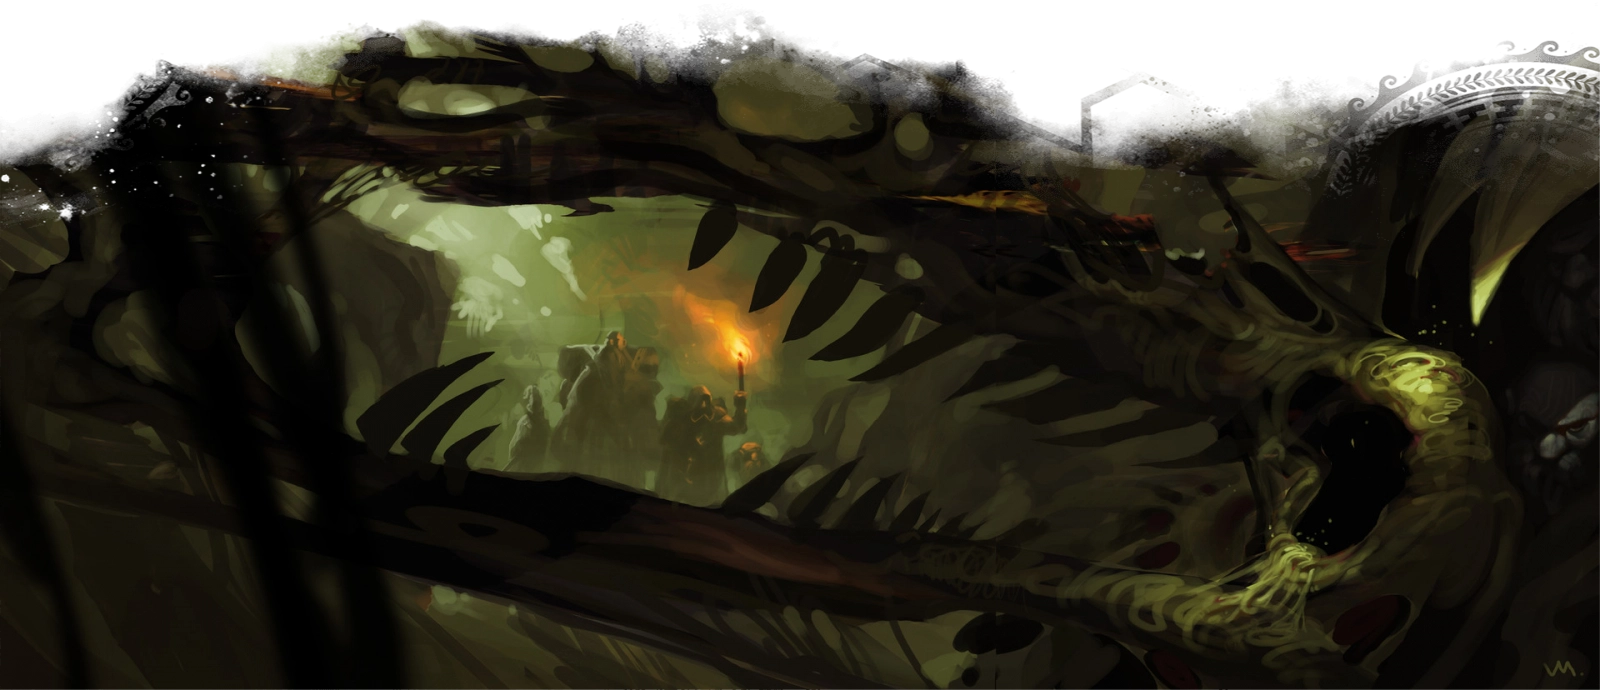
\includegraphics[width=\pdfpagewidth]{03mechanics/img/21jungle_adventure}};
\end{tikzpicture}

\subsubsection{Experience}
    What is learned by your character during the game is measured by Experience Points (XP).
    After you finish playing, talk about the session with the whole group and discuss what happened.
    Read the questions in the table below.
    For each of them that you can reply ``yes'' to, your character gets one XP.

    \begin{itemize}
        \item Did you participate in the session?
        \item Did you travel to a new location?
        \item Did you defeat one or more creatures?
        \item Did you loot treasure?
        \item Did you complete a quest?
        \item Did you solve a conflict?
        \item Did you make a new friend, ally, or enemy?
        \item Did you help another PC?
        \item Did your ideals, bonds, or flaws affect any of your decisions during the session?
        \item Did you perform any action related to your kin, background, or origin?
        \item Did you perform an extraordinary action of some kind?
    \end{itemize}

    In case of any discussion or disagreement, the DM always has the last word.
    Additional XP may be awarded when specific story milestones are achieved, but this too is left to the discretion of the DM.

    \newpage

\subsubsection{Feat Points}
    As your character adventures, they will gain \textbf{Feat Points} (FP).
    Feat points are spent to buy feats, which can only be done as part of a long rest.
    You can buy multiple feats in one long rest.
    Feats either increase your proficiency level at a skill or a proficiency, or they include a useful feature.

    When you reach 10 XP, reset your XP counter and add one FP, keeping the remaining XP.
    Feat points are used to learn new feats, which include either an increase in a proficiency level or a feature.

    You don't need to spend FP right after earning it, you can save as many as you want for as long as you need.
    The full list of feats starts in the next page.

    A new character has a number of FP equal to 3 plus the number of FP that would be required to reach the character's level if it had leveled normally.

\subsubsection{Leveling Up}
    As your character gains feat points they will gain levels, acquiring hit dice, improving their ability scores and saving throw proficiencies, and gaining major character advancements.
    \begin{itemize}
        \item Ability Score Improvements allow you to increase one of you ability scores by 1 up to a maximum of 20.
        \item Saving Throw Improvements increase your level of proficiency on a saving throw of your choice by one, to a maximum of Expert proficiency.
        \item Major Character Advancements are character-defining improvements which include hit dice upgrades, combat styles, and proficiency improvements.
        They are listed in page \pageref{ssec::majorcharacteradvancement}.
    \end{itemize}

    When your Constitution modifier increases by 1 or you improve your hit dice, your hit point maximum increases by 1 for each level you have attained.
    Similarly, you decrease your hit point maximum by 1 if you worsen your hit dice.

    \newpage

% !TEX root = ../main.tex
\subsection*{Major Character Advancement} \label{ssec::majorcharacteradvancement}
Upon reaching levels 3, 11, and 19, your character gains major character advancements.
These are similar to feats, but have stronger effects and are more limited.

\subsubsection{Ability Modifier Improvement} \label{mca::abilitymodifierimprovement}
    Increase an ability modifier of your choice by 2.
    In addition, your maximum for that score is now 24.

\subsubsection{Legendary Proficiency} \label{mca::legendaryproficiency}
    Increase your level of proficiency in two skills or proficiencies to legendary, increasing your proficiency bonus on those skills to +12.
    You must have an expert level of proficiency in both.

\subsubsection{Fighting Style} \label{mca::fightingstyle}
    You learn a fighting style of your choice, or upgrade one that you already know.
    The list of fighting styles is available in page \pageref{ssec::fightingstyles}.

\subsubsection{Hit Die Improvement} \label{mca::hitdieimprovement}
    You increase your hit die from a d6 to a d8, a d8 to a d10, or a d10 to a d12.
    Additionally, you gain a number of hit points equal to your level when you take this major character advancement.

\subsubsection{Spellcasting School} \label{mca::spellcastingschool}
    You join a new spellcasting school from a doctrine different to the one you already follow.
    When you do this, you learn one medium from the new doctrine, and the signature medium and spell from the spellcasting school.

    In addition, you can learn any spell from the new doctrine as you normally would learn a new spell.

\subsubsection{Upgraded Spellcasting} \label{mca::upgradedspellcasting}
    You expand your spellcasting ability beyond its normal limit.
    You reduce your hit die from a d8 to a d6, a d10 to a d8, or a d12 to a d10.
    In addition, you lose a number of hit points equal to your level when you take this major character advancement.

    In exchange for this sacrifice, you gain the ability to cast higher level spells and add more spell points to your pool.
    Your total number of spell points and maximum spell level is available in the table below.

    \begin{DndTable}[width=\linewidth, header=Spellcasting Ability]{XX}
        \textbf{Level} & \textbf{Spell Points} \\
         1st           &   4 \\
         2nd           &   6 \\
         3rd           &  14 \\
         4th           &  17 \\
         5th           &  27 \\
         6th           &  32 \\
         7th           &  38 \\
         8th           &  44 \\
         9th           &  57 \\
        10th           &  64 \\
        11th           &  73 \\
        12th           &  73 \\
        13th           &  83 \\
        14th           &  83 \\
        15th           &  94 \\
        16th           &  94 \\
        17th           & 107 \\
        18th           & 114 \\
        19th           & 123 \\
        20th           & 133
    \end{DndTable}

    \paragraph{Requirements} Spellcaster feat (page \pageref{feat::spellcaster}).

% !TEX root = ../main.tex
\subsection*{Fighting Styles} \label{ssec::fightingstyles}
    \subsubsection{Archery 1}
        You gain a +2 bonus to attack rolls you make with ranged weapons.
    \subsubsection{Archery 2}
        Both your normal and long ranges are multiplied by 1.5 for all ranged weapons.
    \subsubsection{Battle Mastery 1}
        You gain a number a Maneuver Dice equal to half your level (rounded down).
        Your Maneuver Dice are d6s, and are special dice that you can use to enhance the effect of certain actions.
        You regain all expended Maneuver Dice at the end of a short rest.

        Whenever you take an action that involves a d20 roll which isn't the Attack or Cast a Spell action, you can choose to roll a Maneuver Die, adding the result of the die to the d20.
    \subsubsection{Battle Mastery 2}
        You increase the die associated to your Maneuver Dice from a d6 to a d8.

        In addition, when you roll for initiative and have no Maneuver Dice remaining, you regain 4 Maneuver Dice.
    \subsubsection{Dueling 1}
        When you are wielding a melee weapon in one hand and no other weapons, you gain a +2 bonus to damage rolls with that weapon.
    \subsubsection{Dueling 2}
        When you are wielding a melee weapon in one hand and no other weapons, you gain a +1 bonus to AC.
    \subsubsection{Great Weapon Fighting 1}
        When you roll a 1 or 2 on a damage die for an attack you make with a melee weapon that you are wielding with two hands, you can reroll the die and must use the new roll, even if the new roll is a 1 or a 2.
        The weapon must have the two-handed or versatile property for you to gain this benefit.
    \subsubsection{Great Weapon Fighting 2}
        You gain a +1 bonus to attack rolls you make with weapons with the two-handed or versatile property.

        In addition, you gain a +1 bonus to attack rolls you make with weapons with the heavy property.
    \subsubsection{Monastic Fighting 1}
        You gain a number of monastic dice equal to half your level (rounded down).
        Your monastic dice are d6s, and are special dice you can spend to use special abilities related to this fighting style.
        You regain all expended monastic dice at the end of a short rest.

        In addition, you learn three abilities when you learn this fighting style:
        \subparagraph{Concentrated Attack} After you hit a creature with an unarmed attack but before you roll damage for the attack, you can spend one monastic die and add the number rolled to the damage done.
        \subparagraph{Patient Defense} You can spend one monastic die and take the Dodge action using only one action.
        When you do this, add the number rolled to your AC until the start of your next turn.
        \subparagraph{Step of the Wind} You can spend one monastic die to take the Disengage action using only one action.
        When you do this, add the 1.5 times the number rolled to your movement speed (in meters) until the end of your turn.
    \subsubsection{Monastic Fighting 2}
        You increase the die associated to your monastic dice from a d6 to a d8.

        In addition, when you roll for initiative and have no monastic dice remaining, you regain 4 monastic dice.
    \subsubsection{Mounted Fighting 1}
        You have advantage on saving throws made to avoid falling off your mount.
        If you fall off your mount and descend no more than 2 meters, you can land on your feet if you're not incapacitated.

        Finally, mounting or dismounting a creature requires one action rather than two for you.

        To take this fighting style, you must be proficient with land vehicles.
    \subsubsection{Mounted Fighting 2}
        Your steed gains a number of hit points equal to half your maximum hit points.
    \subsubsection{Protection 1}
        While you are wearing armor, you gain a +1 bonus to AC.
    \subsubsection{Protection 2}
        You gain a bonus to all Strength, Dexterity, and Constitution saving throws equal to the AC granted by your shield.
    \subsubsection{Thrown Weapon Fighting 1}
        You can draw a weapon that has the thrown property as part of the attack you make with the weapon.
    \subsubsection{Thrown Weapon Fighting 2}
        When you hit with a ranged attack using a thrown weapon, you add a +2 bonus to the damage roll.
    \subsubsection{Two-Weapon Fighting 1}
        You suffer from the multiple attack penalty for each wielded weapon independently --- Attack rolls made with a weapon held in one hand don't impose a penalty on attack rolls made with a weapon held in your other hand.
    \subsubsection{Two-Weapon Fighting 2}
        When you engage in two-weapon fighting, you can add your ability modifier to the damage of the second attack.
    \subsubsection{Unarmed Fighting 1}
        Your unarmed strikes can deal bludgeoning damage equal to 1d6 + your Strength modifier on a hit.

        In addition, the multiple attack penalty is reduced by 1 when you make unarmed attacks.
    \subsubsection{Unarmed Fighting 2}
        If you aren't wielding any weapons or a shield, the damage die from your unarmed strikes becomes a d8.

        In addition, you can deal 1d4 bludgeoning damage to one creature grappled by you at the start of each of your turns.

\newpage

% % !TEX root = ../main.tex
\section{Feats}
For simplicity, feats are separated into six categories: feats related to kin, background, skills, proficiencies, combat, and spellcasting.
Each category is listed in the following pages.
Categories are ordered alfabetically, but each is listed in an easy to follow fashion in their respective sections.

Unless specified otherwise, a feat can only be learned once.

% TODO: Write list of Fighting Styles and ``Casting Styles'' (Based on this: https://standsinthefire.com/2016/05/31/dd-5e-magical-styles/).
% TODO: Combat maneuvers, metamagic options and other **don't have a point system associated to them**. They simply add effects to attacks or spellcasting by using one additional action!
% TODO: Write Combat Maneuvers section.
% TODO: Write list of Metamagic Options.

% !TEX root = ../main.tex
\subsection*{Kin Feats}
% TODO: LIST KINS AND THEIR ASSOCIATED FEATS. IT'LL MAKE THINGS EASIER FOR EVERYONE.

% A
\subsubsection{Acid Spit} \label{feat::acidspit}
    By repeatedly feeding on toxic tree leaves, your saliva has become as vile as its poison.
    You can use two actions to spit a 1.5 by 9 meters line of acid.
    Every target in the area must make a Dexterity saving throw, with a DC of 8 + your Constitution modifier.
    A creature takes 2d6 acid damage on a failed save, or half as much damage on a successful one.
    The acid damage increases to 3d6 with your 6th level, 4d6 with your 11th, and 5d6 with your 16th.
    You can use this trait a number of times equal to your Constitution modifier (Minimum of 1) per short rest.

    You can take this feat three additional times, increasing the DC by 2 each time.
    \paragraph{Requirements} Marset kin.
\subsubsection{Adaptable} \label{feat::adaptable}
    You gain one feat that costs 1 FP from any background.
    \paragraph{Requirements} Quies kin or Common Uman subrace.
\subsubsection{Aerial Defense (2 FP)} \label{feat::aerialdefense}
    Creatures who attack you while you're falling, flying, gliding, or jumping have disadvantage on their attack roll.
    \paragraph{Requirements} Ird kin.
\subsubsection{Alert} \label{feat::alert}
    Always in the lookout for danger, you gain a +5 bonus to initiative and you can't be surprised while conscious.
    \paragraph{Requirements} Uman kin.
\subsubsection{Arboreal Alertness} \label{feat::arborealalertness}
    As long as you are not already an Expert, you increase your level of competence in the Perception skill.
    Additionally, you gain a +5 bonus to your passive Wisdom (Perception) and passive Wisdom (Insight) when in forested areas.
    \paragraph{Requirements} Grung kin or Boggart subrace.
\subsubsection{Arctic Temperature (2 FP)} \label{feat::arctictemperature}
    You are immune to cold damage.
    In addition, after receiving an attack that would have dealt cold damage you can use your \textbf{Cryogenic Stillness} trait without expending a use as a reaction, but you can only remain cold until the end of your next turn.
    \paragraph{Requirements} Hail Zaloth subrace.
\subsubsection{Automatic Cleansing} \label{feat::automaticcleansing}
    Your body automatically processes the harshest of poisons.
    You are immune to poison damage and the poisoned condition.
    \paragraph{Requirements} Quies kin.
\subsubsection{Automatic Nutrition} \label{feat::automaticnutrition}
    When in fertile land, you don't need to eat.

    Additionally, you can enter a state of hibernation as part of a short rest, becoming indistinguishable from a large plant.
    While hibernating you don't age, and are aware of your surroundings.
    You cannot use any actions, except to take an action to wake up at will.
    \paragraph{Requirements} Naenk kin.
% B
\subsubsection{Balm of Dreams} \label{feat::balmofdreams}
    You learn how to excrete a healing balm from your fungal growths.
    You have a pool of balm represented by a number of d4s equal to your level.

    As an action, you can choose one creature you can see withint 1.5 meters of you and spend a number of those dice equal to half your level or less.
    Roll the spent dice and add them together.
    The target regains a number of hit points equal to the total.
    The target also gains 1 temporary hit point per die spent.

    This balm is uneffective on tsaneks.
    You regain all expended dice when you finish a short rest.
    \paragraph{Requirements} Gannagian Tsanek subrace.
\subsubsection{Benign Growths (2 FP)} \label{feat::benigngrowths}
    As part of a short rest, you can grow a fungal cornucopia on your back.
    The growths correspond to 3 doses, each of which can be consumed by expending 2 actions.
    Each growth has a random special effect, which is decided randomly by rolling a d6 during the short rest taken:
    \begin{DndTable}[width=\linewidth, header=Benign Growths]{cX}
        \textbf{d6} & \textbf{Effect} \\
        1  & \textbf{Healing}. The creature's regains a number of hit points equal to 2d4 + your Constitution modifier. \\
        2  & \textbf{Swiftness}. The creature's walking speed increases by 3 meters for 10 minutes. \\
        3  & \textbf{Resilience}. The creature gains a +1 bonus to AC for 10 minutes. \\
        4  & \textbf{Boldness}. The creature can roll a d4 and add the number rolled to every attack roll and saving throw they make for the next minute. \\
        5  & \textbf{Sporing} The creature gains the \textbf{Pacifying Spores} trait (see page \pageref{kin::tsanek.pacifyingspores}) for 10 minutes. \\
        5  & \textbf{Melding}. The creature can meld with you on your next short rest.
        You both gain the effect associated to melding (see page \pageref{kin::tsanek.meld}).
    \end{DndTable}
    Apart from their effect, each growth comfortably feeds a creature for a day.
    \paragraph{Requirements} Na'anian Tsanek subrace.
\subsubsection{Bone Breaker} \label{feat::bonebreaker}
    While gliding, you can attempt to attack a creature with an eviscerating attack.
    Using two actions, you can swoop down up to your movement speed towards a creature you can see, and make a melee weapon attack roll against it.
    If the attack hits, it's a critical hit.
    The attack is tiring, and you can use this feat only once per combat encounter.
    \paragraph{Requirements} Sunstruck Oth subrace.
\subsubsection{Born Climber} \label{feat::bornclimber}
    You can use your tail to grab onto branches, and don't require to pass any ability checks to climb.
    Additionally, you are able to freely use your hands while climbing, and you increase your climbing speed by three meters.
    \paragraph{Requirements} Marset kin.
\subsubsection{Born Grappler} \label{feat::borngrappler}
    You don't need to have a hand free to grapple, using both your extra arms to do so.
    If you do have a free arm, you roll for the grapple check with advantage.
    You cannot use this feat if you are holding something in one or both of your extra arms.
    \paragraph{Requirements} Oth kin.
\subsubsection{Bountiful Luck (2 FP)} \label{feat::bountifulluck}
    Your people have extraordinary luck, which you have learned to lend to your companions when you see them falter.
    You're not sure how you do it; you just wish it, and it happens.
    Surely a sign of fortune's favor!

    When an ally you can see within 9 meters of you rolls a 1 on the d20 for an attack roll, an ability check, or a saving throw, you can use your reaction to let the ally reroll the die.
    The ally must use the new roll.

    When you use this ability, you can't use your Fated trait before the end of your next turn.
    \paragraph{Requirements} Chu'ash Oth subrace.
% C
\subsubsection{Cellular Regeneration} \label{feat::cellularregeneration}
    As an action, you can stimulate your plant cells to rapidly multiply to quickly regenerate wounds.
    You regain 1 hit point, and regain 1 hit point at the start of each of your turns after, until you've restored an amount equal to twice your level.
    After using this trait, you must take a long rest before using it again.
    If you suffer cold, fire, or necrotic damage, this regeneration is cancelled.
    You are also able to regenerate lost limbs, albeit at a very slow pace: it takes you 1d4+2 months to fully recover a lost arm or leg.
    \paragraph{Requirements} Naenk kin.
\subsubsection{Communal} \label{feat::communal}
    Whenever you make an Intelligence (History) check related to the history of your kin, culture, or community, you are considered of Legendary proficiency in the History skill, adding a proficiency bonus of +12 to the check instead of your normal proficiency bonus in the skill.
    \paragraph{Requirements} Marset kin.
\subsubsection{Cosmic Omen} \label{feat::cosmicomen}
    It is said that zaloths have a special connection to the cosmos.
    As part of a short rest, you can consult the starts for omens.
    When you do so, roll a die.
    Until you finish your next short rest, you gain access to a special reaction based on whether you rolled an even or an odd number on the die:
    \begin{itemize}
        \item \textbf{Weal (even).} Whenever a creature you can see within 9 meters of you is about to make an attack roll, a saving throw, or an ability check, you can use your reaction to roll a d6 and add the number rolled to the total.
        \item \textbf{Woe (odd).} Whenever a creature you can see within 9 meters of you is about to make an attack roll, a saving throw, or an ability check, you can use your reaction to roll a d6 and subtract the number rolled from the total.
    \end{itemize}
    You can use this ability a number of times equal to your Charisma modifier (minimum of once), and regain all expended uses on a short rest.
    \paragraph{Requirements} Zaloth kin.
\subsubsection{Cower!} \label{feat::cower}
    As a reaction, you can quickly cower into your shell, activating your \textbf{Shell Defense} trait.
    If you use this trait when you are subjected to an effect that allows you to make a Dexterity saving throw to take only half damage, you automatically succeed on the saving throw.
    \paragraph{Requirements} Tortle kin.
\subsubsection{Curl Up (2 FP)} \label{feat::curlup}
    You can use one action to curl up, exposing attackers to a wall of your toughened quills.
    While curled up in this way you cannot move, attack, or cast spells with somatic components, and your base armor class becomes 19.
    You cannot benefit from any Dexterity bonus to armor class while curled up, but you can still use shields.

    Any creature that misses you with a melee attack while you are curled up takes 2d8 + your Dexterity modifier piercing damage from your sharp spines.
    You may uncurl as a free action at any point during your turn.
    \paragraph{Requirements} Marset kin.
% D
\subsubsection{Danger Sense} \label{feat::dangersense}
    Accustomed to being hunted, you gain an uncanny sense of when things nearby aren't as they should be, giving you an edge when you dodge away from danger.
    You have advantage on Dexterity saving throws against effects that you can see, such as traps and spells.
    To gain this benefit, you can't be blinded, deafened, or incapacitated.
    \paragraph{Requirements} Uman kin.
\subsubsection{Deadly Grip} \label{feat::deadlygrip}
    While flying, you have advantage on Grapple checks made with your talons.
    \paragraph{Requirements} Ird kin.
\subsubsection{Deadly Precision (2 FP)} \label{feat::deadlyprecision}
    Whenever you have advantage on an attack roll using Dexterity, Intelligence, Wisdom, or Charisma, you can reroll one of the dice once.
    Additionally, you learn the Aim action.
    \paragraph{Requirements} Dratl Ird or Sunstruck Oth subrace.
\subsubsection{Deft Hands} \label{feat::defthands}
    Any Dexterity (Sleight of Hand) check or check with any set of tools you make gains a +1 bonus.
    \paragraph{Requirements} Common Uman or Quies Operative subrace.
\subsubsection{Depths of Nerono} \label{feat::depthsofnerono}
    % NOTE: Nerono is the ``ocean'' plane of Nyx.
    When you roll cold damage for a spell you cast, you can reroll any roll of 1 on the cold damage dice, but you must use the new roll, even if it is another 1.

    In addition, whenever you cast a spell that deals cold damage, you can cause ice to envelop you until the end of your next turn.
    While the ice is present, you gain a +2 bonus to AC, and creatures within 1.5 meters of you (including you) are affected by the \textbf{Slow} spell.
    \paragraph{Requirements} Frostburn Nomad or Hail Zaloth subrace.
\subsubsection{Designed with a Purpose (2 FP)} \label{feat::designedwithapurpose}
    Following your creator's design, your competence at a particular skill is unparalleled.
    Your proficiency with a skill is increased to Legendary, increasing your proficiency bonus to +12 with it.
    \paragraph{Requirements} Quies Operative subrace. Expert proficiency with a skill.
\subsubsection{Displace Teleportation} \label{feat::displaceteleportation}
    As a reaction, when a creature within 18 meters of you attempts to teleport, you can foil the teleportation attempt.
    The target reappears in an empty space within 1.5 meters of your, and takes 1d12 thunder damage.
    \paragraph{Requirements} Thunder Zaloth subrace.
% E
\subsubsection{Efficient Craftsgat} \label{feat::efficientcraftsgat}
    They say that a gat is born with tools in their hands.
    Crafting times with the artisan's tools related to your craftgatship trait are halved for you.
    \paragraph{Requirements} Gat kin.
\subsubsection{Enhanced Claws} \label{feat::enhancedclaws}
    By manipulating your biology, you can improve your claws to become deadly weapons.
    You change the damage die from your claws to the following one, so that a d4 changes into a d6, a d6 into a d8, a d8 into a d10, or a d10 into a d12.

    You can take this feat three times, improving the damage die by the described amount.
    \paragraph{Requirements} Naenk kin.
\subsubsection{Enhanced Spores} \label{feat::enhancedspores}
    You can add a +2 bonus to all of your spore effects' spell save DC.
    % Alternatively, you can add your spellcasting modifier if you have one.

    You can take this feat three times.
    \paragraph{Requirements} Tsanek kin.
\subsubsection{Exercised Mind (2 FP)} \label{feat::exercisedmind}
    Generational learning has taught you that a qualar is only as strong as your will is.
    You are naturally good staving off dementia.
    You can choose to change the Dementia saving throw (see page \pageref{ssec::dementia}) from Intelligence to Wisdom, and its DC is 12 for you.
    Additionally, if you succeed on the saving throw, you reduce your dementia level by 1.
    \paragraph{Requirements} Bughna Gat subrace.
% F
\subsubsection{Fade Out} \label{feat::fadeout}
    As an action or reaction, you can disperse into a 1.5-meter cloud of smoke until the end of your next turn.
    While in this form you cannot take damage, and the only action you can take is to move up to your moving speed.
    You can pass through creatures while in this shape, and if you do so the creature must succeed on a DC 12 Constitution saving throw, becoming incapacitated until the end of their next turn on a failure.

    While in this shape, you are forced to move with the wind, and any spell that controls it (such as \textbf{Gust of Wind}) can move you against your will.

    Once you use this ability, you cannot use it again until you finish a short rest.
    \paragraph{Requirements} Gale Zaloth or Ash Zaloth subrace.
\subsubsection{Fast as Lightning} \label{feat::fastaslightning}
    As an action on your turn, you can teleport up to 18 meters to an unoccupied space you can see.
    Alternatively, you can use this action to teleport one willing creature you touch up to 9 meters to an unoccupied space you can see.
    This movement is accompanied by the roaring sound of thunder that can be heard up to a distance of 36 meters.

    You can use this feature a number of times equal to your Charisma modifier (Minimum of once), and you regain all expended uses of it when you finish a short rest.
    \paragraph{Requirements} Thunder Zaloth subrace.
\subsubsection{Fey Touched} \label{feat::feytouched}
    You learn the misty step (see page \pageref{spell::mistystep}) and one 1st-level spell of your choice.
    The spell must be from the Sympathy doctrine.
    You can cast each of these spells without expending a spell slot.
    Once you cast either of these spells in this way, you can't cast that spell in this way again until you finish a short rest.
    You can also cast these spells using spell slots you have of the appropriate level.
    The spells' spellcasting ability is Intelligence.
    \paragraph{Requirements} Chu'ash Oth subrace.
\subsubsection{Flames of Tizerus} \label{feat::flamesoftizerus}
    % NOTE: Tizerus is the ``hellish'' plane of Nyx.
    When you roll fire damage for a spell you cast, you can reroll any roll of 1 on the fire damage dice, but you must use the new roll, even if it is another 1.

    In addition, whenever you cast a spell that deals fire damage, you can cause flames to wreathe you until the end of your next turn.
    The flames don't harm you or your possessions, and they shed bright light out to 9 meters and dim light for an additional 9 meters.
    While the flames are present, any creature within 1.5 meters of you that hits you with a melee attack takes 1d4 fire damage.
    \paragraph{Requirements} Ash Zaloth or Quies Slag Worker subrace.
\subsubsection{Fleet of Foot} \label{feat::fleetoffoot}
    Your base walking speed increases by 1.5 meters.
    \paragraph{Requirements} Uman kin or Quies Operative subrace.
\subsubsection{Force of Will} \label{feat::forceofwill}
    You can plant yourself in place with all your weight, making you very difficult to move.
    As long as your feet are on the ground, you have advantage on any ability checks or saving throws made to move you or force you to fall prone.
    \paragraph{Requirements} Gat or Quies kin.
\subsubsection{Forest Defender} \label{feat::forestdefender}
    You have received martial training to fight among the branches, and are extremely dangerous to climbing opponents.
    You know the Push action (See page \pageref{act::push}), and the target rolls the saving throw with disadvantage if you climbed, glided, or flew at least 3 meters this turn.
    \paragraph{Requirements} Qulbaba Ird or Marset kin.
\subsubsection{Fungal Abode} \label{feat::fungalabode}
    Spending a minute to communicate with the ground, you bring forth a 3 meter dome-shaped hollow fungus from mycelium.
    Nine creatures of Medium size or smaller can fit inside the dome with you.
    The atmosphere inside the fungus is humid, making it slightly uncomfortable for most creatures.
    The interior is dimly lit.

    The dome has an AC of 8 and an HP of 15, and lasts for 8 hours.
    After this time or if the dome is destroyed, it returns to the mycelium.
    \paragraph{Requirements} Tsanek kin or Na'anian Naenk subrace.
\subsubsection{Fungal Body} \label{feat::fungalbody}
    Your normal sight and hearing are extended by the spores around you.
    You gain truesight to a range of 3 meters, and become immune to the blinded and deafened conditions.
    \paragraph{Requirements} Tsanek kin.
\subsubsection{Fungal Infestation (2 FP)} \label{feat::fungalinfestation}
    Your spores gain the ability to infest a corpse and animate it.
    If a beast or a humanoid that is Small or Medium dies within 3 meters of you, you can use your reaction to animate it, causing it to stand up immediately with 1 hit point.
    The creature uses the zombie stat block in the Monster Manual.
    It remains animate for 1 hour, after which time it collapses and dies.

    In combat, the zombie's turn comes immediately after yours.
    It obeys your mental commands, and the only action it can take is the Attack action, making one melee attack.

    You can use this feature a number of times equal to your Wisdom modifier (minimum of once), and you regain all expended uses of it when you finish a short rest.
    \paragraph{Requirements} Gannagian Tsanek subrace.
% G
\subsubsection{Gat Resilience (2 FP)} \label{feat::gatresilience}
    The horned kin possesses an almost otherwordly hardiness.
    You have advantage on saving throws against poison and disease.
    In addition, you are resistant against poison damage.
    \paragraph{Requirements} Noves Gat subrace.
\subsubsection{Gelid Aura} \label{feat::gelidaura}
    As an action, you can choose to activate a gelid aura around you, replacing your natural radiance for a minute or until you decide to end the effect as an action.
    At the end of each of your turns for that duration, each creature within 1.5 meters of you takes cold damage equal to 1d6 + half your level (rounded down).
    \paragraph{Requirements} Hail Zaloth subrace.
\subsubsection{Giant Slayer (2 FP)} \label{feat::giantslayer}
    An apprentice of the giant slayers from the north, your skill with heavy weapons is unparalleled.
    You gain a +2 bonus to attack rolls made with heavy weapons, and learn the Reckless Attack action (see page \pageref{act::recklessattack}).
    \paragraph{Requirements} Thulkraka ird subrace.
\subsubsection{Goat's Strength} \label{feat::goatsstrength}
    You complement your natural strengths with hard training.
    The DC related to the Push action gains a +2 bonus for you.
    Additionally, any attack made with your horns gains a +2 to its attack rolls.

    You can take this feat three times.
    \paragraph{Requirements} Gat kin.
\subsubsection{Gold Toxin} \label{feat::goldtoxin}
    You learn how to excrete the rarest of grung poisons, the gold toxin.
    Once per long rest, you can choose to use a gold toxin when you use your poisonous skin trait.
    The DC from your \textbf{Poisonous Skin} trait increases by 2, and on a failure the creature is charmed for a minute.
    The creature can repeat this saving throw at the end of its turns.
    Additionally, it permanently learns how to speak basic krehlo.
    \paragraph{Requirements} Grung kin.
\subsubsection{Goring Rush} \label{feat::goringrush}
    If you move at least 6 meters towards a creature, you can make one melee attack or use the Push action with your horns against the creature as a free action.
    \paragraph{Requirements} Treb Gat subrace.
\subsubsection{Graceful Pass} \label{feat::gracefulpass}
    Using your wings to aid your movement, difficult terrain doesn't cost you extra movement.
    \paragraph{Requirements} Ird or Oth kin.
% H
\subsubsection{Hardy} \label{feat::hardy}
    Resilience comes as natural to you as breathing.
    As long as you are not already an expert, you increase your proficiency in the Survival skill.
    Additionally, you can choose to add your Constitution modifier to Survival ability checks instead of your Wisdom modifier.
    \paragraph{Requirements} Bughna Gat or Gannagian Warrior subrace or Grung kin.
\subsubsection{Halo of Spores} \label{feat::haloofspores}
    You are surrounded by invisible, necrotic spores that are harmless until you unleash them on a creature nearby.
    When a creature you can see moves into a space within 3 meters of you or starts its turn there, you can use your reaction to deal 1d4 necrotic damage to that creature unless it succeeds on a Constitution saving throw against a DC of 8 + your Constitution modifier.
    The necrotic damage increases to 1d6 at 6th level, 1d8 at 10th level, and 1d10 at 14th level.
    \paragraph{Requirements} Na'anian Naenk or Na'anian Tsanek subrace.
\subsubsection{Horned Fury} \label{feat::hornedfury}
    Your fury burns tirelessly.
    You gain the following benefits:
    \begin{itemize}
        \item When you hit with an attack using a melee weapon or unarmed strike, you can roll one of the weapon's damage dice an additional time and add it as extra damage of the weapon's damage type.
        Once you use this ability, you can't use it again until you finish a short rest.
        \item Immediately after you use your Relentless Endurance trait, you can use your reaction to make one weapon attack.
    \end{itemize}
    \paragraph{Requirements} Cursed Uman subrace.
% I
\subsubsection{Immutable Form} \label{feat::immutableform}
    Embracing your origin, you become protected by the strange designs of the tall kin.
    You are immune to any effect that would alter your form.
    \paragraph{Requirements} Quies kin.
\subsubsection{Impaling Carapace} \label{feat::impalingcarapace}
    Through careful training, you know how to position your natural armor for deadly effect in combat.
    When you grapple a creature, the target takes 3 piercing damage if your grapple check succeeds.
    If another creature grapples you, it takes 3 piercing damage.
    If you start your turn grappling or being grappled by a creature, it takes 3 piercing damage.
    \paragraph{Requirements} Marset or Tortle kin or Frostburn Nomad subrace.
\subsubsection{Imposing Presence (2 FP)} \label{feat::imposingpresence}
    You increase your proficiency level in Intimidation or Persuasion to Legendary, increasing your proficiency bonus to +12.
    \paragraph{Requirements} Treb Gat or Cursed Uman subrace. Expert proficiency in the chosen skill.
\subsubsection{Improved Nuen (2 FP)} \label{feat::improvednuen}
    Your nuens are stronger than average, and you do not half the creature's hit points or hit dice when you raise one.
    Additionally, your nuen grows a thick layer of thorns, gaining the \textbf{Impaling Carapace} feat (see page \pageref{feat::impalingcarapace}).
    \paragraph{Requirements} Gannagian Warrior subrace.
\subsubsection{Improved Plant Camouflage} \label{feat::improvedplantcamouflage}
    You have advantage in Dexterity (Stealth) checks you make, using your mutable form to mimic an object in the environment.
    \paragraph{Requirements} Gannagian Hunter subrace.
\subsubsection{Integrated Weapon} \label{feat::integratedweapon}
    Your understanding of your own body allows you to modify it with ease.
    As part of a short rest, you can integrate a weapon into your form.
    You can only have one weapon integrated at a time, and you can separate from it as part of a short rest.

    You can equip and unequip your integrated weapon as a free action, and don't provoke opportunity attacks when equipping it.
    When inactive, the weapon is effectively invisible, requiring no check of any kind to conceal.

    You can take this feat two additional times.
    The second time gives you a +1 bonus to damage rolls made with the weapon.
    The third time allows you to make a melee attack as part of the free action used to equip your weapon.
    This attack increases the multiple attack penalty as normal.
    \paragraph{Requirements} Quies kin.
% J
% K
\subsubsection{Keen Mind} \label{feat::keenmind}
    You always know which way is north, and you can always know the number of hours left before the next sunrise or sunset.
    \paragraph{Requirements} Oth kin.
\subsubsection{Keenest Senses (2 FP)} \label{feat::keenestsenses}
    You increase your proficiency level with Insight, Investigation, or Perception from Expert to Legendary, increasing your proficiency bonus with the skill to +12.
    \paragraph{Requirements} Qulbaba Ird or Boggart subrace.
% L
\subsubsection{Last Resort} \label{feat::lastresort}
    Immediately after you use your \textbf{Relentless Endurance} trait, you can use your reaction to move up to your movement speed in a mad rush for survival.
    This movement doesn't provoke opportunity attacks.
    \paragraph{Requirements} Uman kin.
\subsubsection{Legendary Craftsgat (2 FP)} \label{feat::legendarycraftsgat}
    Above the average gat, you are legendary at the use of your tools.
    Your proficiency with the artisan's tools related to your craftgatship trait is increased to Legendary, incresing your proficiency bonus to +12 with them.
    \paragraph{Requirements} Gat kin. Expert proficiency with a set of artisan's tools.
\subsubsection{Linguist} \label{feat::linguist}
    You have studied languages and codes, gaining the following benefits:
    \begin{itemize}
        \item You learn a language of your choice.
        \item You can ably create written ciphers.
        Others can't decipher a code you create unless you teach them, they succeed on an Intelligence check (DC equal to 6 + your Intelligence score), or they use magic to decipher it. % TODO: Figure out what spell (probably from Dremshamad) would be able to do this.
    \end{itemize}
    \paragraph{Requirements} Moonborn Oth subrace.
\subsubsection{Lip Reading} \label{feat::lipreading}
    If you can see a creature's mouth while it is speaking a language you understand, you can understand what it's saying by reading its lips.
    \paragraph{Requirements} Marset kin.
\subsubsection{Long-Limbed (2 FP)} \label{feat::longlimbed}
    You harness your inherited adaptability, learning how to alter your proportions at will.
    When you make a melee attack on your turn, your reach for it is 1.5 meters greater than normal.
    \paragraph{Requirements} Quies kin.
\subsubsection{Lucky} \label{feat::lucky}
    When you roll a 1 on an attack roll, ability check, or saving throw, you can reroll the die and must use the new roll.
    This doesn't count as a use of the Fated trait.
    \paragraph{Requirements} Tortle kin or Chu'ash Oth subrace.
% M
\subsubsection{Magic Initiate (2 FP)} \label{feat::magicinitiate}
    Your learn two cantrips of your choice from one spellcasting doctrine of your choice.
    In addition, choose one 1st-level spell from the same doctrine.
    You learn that spell and can cast it at its lowest level.
    Once you cast it, you must finish a long rest before you can cast it again using this feat.
    Your spellcasting ability for these spells is Intelligence.
    \paragraph{Requirements} Moonborn Oth subrace.
\subsubsection{Master Gatherer (2 FP)} \label{feat::mastergatherer}
    You increase your proficiency with a herbalism kit to Legendary, increasing your proficiency bonus with it to +12.
    \paragraph{Requirements} Gannagian Gatherer subrace. Expert proficiency with a herbalism kit.
\subsubsection{Mesmerizing Chirr (2 FP)} \label{feat::mesmerizingchirr}
    You make a chirring noise to which grungs are immune.
    Each humanoid or beast that is within 4.5 meters of you and able to hear you must succeed on a DC 10 + your Constitution modifier Wisdom saving throw or be stunned until the end of your next turn.
    You can use this ability a number of times equal to your Constitution modifier (minimum of 1), and recover all expended uses at the end of a short rest.
    \paragraph{Requirements} Grung kin.
\subsubsection{Mirthful Leaps} \label{feat::mirthfulleaps}
    Whenever you make a long or high jump, you can roll a d4 and add the number rolled to the number of meters you cover, even when making a standing jump.
    This extra distance costs movement as normal.
    \paragraph{Requirements} Bughna Gat or Grung kin.
\subsubsection{Moist Skin} \label{feat::moistskin}
    As an action or reaction, you can choose to rapidly excrete a large amount of water from your skin.
    When you do this, you gain resistance to fire damage and vulnerability to cold damage for until the end of your next turn.
    You can use this ability a number of times equal to your Constitution modifier (Minimum of one).
    \paragraph{Requirements} Grung kin.
\subsubsection{Moss Armor} \label{feat::mossarmor}
    Your plant-based framework provides you with unique resilience.
    You have resistance against lightning damage.
    % You have advantage on saving throws against paralysis and are resistant to lightning damage.
    \paragraph{Requirements} Naenk kin.
\subsubsection{Mountain Born} \label{feat::mountainborn}
    You are acclimated to high altitude.
    You don't suffer the effects associated to the cold or lack of oxygen of any elevation up to 10,000 meters.
    You also have a climbing speed of 6 meters.
    \paragraph{Requirements} Noves Gat or Thulkraka Ird subrace.
\subsubsection{Mycelium Connection} \label{feat::myceliumconnection}
    As an action, you can establish a connection with a creature within 9 meters of you.
    Roll a Wisdom (Insight) check contested by the creature's Wisdom (Insight).
    The creature can choose to fail on this save on purpose.
    If you succeed, you know the location of the creature and can telepathically communicate with it for 24 hours.
    The creature knows that it is connected to you, as it feels your presence pulsating in its head, but it cannot end this connection.

    This ability only works while the creature is touching the ground.
    \paragraph{Requirements} Tsanek kin.
% N
\subsubsection{Narcotic Empowerement} \label{feat::narcoticempowerement}
    From your training as a shaman, you are able to release special chemicals as part of your meditation.
    With an hour of rest, you choose expended spell slots to recover.
    The spell slots can have a combined level that is equal to or less than half your level (rounded up), and none of the slots can be 6th level or higher.
    You can't use this feature again until you finish a short rest.

    For example, when you are 4th-level, you can recover up to two levels worth of spell slots.
    You can recover either a 2nd-level slot or two 1st-level slots.
    \paragraph{Requirements} Gannagian Tsanek subrace.
\subsubsection{Natural Forager} \label{feat::naturalforager}
    Due to your nature as a gatherer, all foraging DCs are reduced by 5 for you.
    You can also feed on tree gum, but cannot cook meals for other species with this material.
    \paragraph{Requirements} Marset or Gannagian Gatherer kin.
\subsubsection{Nature's Sanctuary} \label{feat::naturessanctuary}
    Creatures of the natural world sense your connection to nature and become hesitant to attack you.
    When a beast or plant creature attacks you, that creature must make a Wisdom saving throw with a DC of 12.
    On a failed save, the creature must choose a different target, or the attack automatically misses.
    On a successful save, the creature is immune to this effect for 24 hours.

    The creature is aware of this effect before it makes its attack against you.
    \paragraph{Requirements} Naenk or Tsanek kin.
\subsubsection{Nimble and Deadly (2 FP)} \label{feat::nimbleanddeadly}
    You can move through the space of any creaturee that is of a size larger than you.
    When you do so, the creature takes 3 piercing damage.
    \paragraph{Requirements} Marset kin.
\subsubsection{Nimble Step} \label{feat::nimblestep}
    Opportunity attacks made against you are rolled with disadvantage.
    \paragraph{Requirements} Ird Kin or Gale Zaloth subrace.
% O
\subsubsection{Observant} \label{feat::observant}
    You gain a +5 bonus to your passive Wisdom (Perception) and passive Intelligence (Investigation) scores.
    \paragraph{Requirements} Moonborn Oth or Na'anian Tsanek subrace.
\subsubsection{One with the Wind (2 FP)} \label{feat::onewiththewind}
    You increase your movement speed by 3 meters.
    Additionally, you double your movement speed when moving in the direction of a spell that controls wind, such a \textbf{Gale}.
    \paragraph{Requirements} Gale Zaloth subrace.
\subsubsection{Overheating (2 FP)} \label{feat::overheating}
    You are immune to fire damage.
    Additionally, You can radiate excess heat around you as an action.
    For 1 minute, all creature that start their turn within 1.5 meters of you take 1d6 fire damage from this heat.

    You can use this ability a number of times equal to your Constitution modifier (minimum of 1), and regain all expended uses on a short rest.
    \paragraph{Requirements} Quies Slag Worker subrace.
\subsubsection{Overpressure (2 FP)} \label{feat::overpressure}
    You gain immunity to fire damage and vulnerability to cold damage.
    Using two actions, you can switch these, gaining immunity to cold damage and vulnerability to fire damage or the other way around.
    \paragraph{Requirements} Quies Juggernaut subrace.
% P
\subsubsection{Patient} \label{feat::patient}
    When you react with a readied action, you have advantage on the first die roll you make as part of that action.
    \paragraph{Requirements} Dratl Ird subrace.
\subsubsection{Perfect Landing} \label{feat::perfectlanding}
    Furthering your natural falling skills, you are trained to handle any fall with ease.
    As long as you are conscious and can freely use your wings, you are immune to fall damage.
    \paragraph{Requirements} Ird kin.
\subsubsection{Poison Immunity} \label{feat::poisonimmunity}
    You've developed your poison resistance from constant exposure to poisons in your environment and from your own skin.
    You are immune to poison damage and the poisoned condition.
    \paragraph{Requirements} Grung kin.
\subsubsection{Poisoned Claws} \label{feat::poisonedclaws}
    When you hit a creature with an unarmed strike using your claws, the creature must roll on a DC 12 Constitution saving throw.
    On a failed save, the creature is poisoned.
    The creature can repeat this saving throw at the end of its turns, ending the poisoned conditions on a successful save.
    \paragraph{Requirements} Gannagian Warrior subrace.
\subsubsection{Powerful Build} \label{feat::powerfulbuild}
    You count as one size larger when determining your carrying capacity and the weight you can push, drag, or lift.
    \paragraph{Requirements} Gat or Tortle kin.
\subsubsection{Predestined} \label{feat::predenstined}
    Once per day you can choose to reroll an attack, skill check, or saving throw.
    You can decide to do this after the roll, but before the outcome of the roll has been determined.
    If you are a Chu'ash oth, consider your Fated trait as one additional use of this feat.

    You can learn this trait 3 times, increasing the number of times you can use this feat per day by one each time.
    On the third time, you gain the ability to use this trait to force an enemy to reroll an attack roll made against you.
    \paragraph{Requirements} Oth kin.
\subsubsection{Primeval Awareness} \label{feat::primevalawareness}
    You can use an action to focus your awareness on the region around you.
    For 1 minute, you can sense all creatures that aren't plants or beasts present within 1 kilometer of you.
    This feat doesn't reveal the creatures' exact location or number, but it gives you a hint of their position in relation to you.

    You can use this feature a number of times equal to your Wisdom modifier (minimum of once).
    \paragraph{Requirements} Naenk kin or Boggart subrace.
\subsubsection{Prodigy (2 FP)} \label{feat::prodigy}
    Choose one skill in which you are an Expert.
    You increase your proficiency in that skill to Legendary, increasing your proficiency bonus to +12.
    \paragraph{Requirements} Common Uman subrace. Expert proficiency in the selected skill.
\subsubsection{Protected but Dangerous (2 FP)} \label{feat::protectedbutdangerous}
    While using your \textbf{Shell Defense} trait, you can perform any action that doesn't involve your hands or legs.
    For example, you can cast spells without somatic components, or use the \textbf{Steam Breath} action if you know it.
    \paragraph{Requirements} Tortle kin.
\subsubsection{Purity of Body} \label{feat::purityofbody}
    Tortle culture involves a strong culinary tradition, enhancing your body's natural healing ability.
    You have advantage on saving throws against poison and disease.
    \paragraph{Requirements} Tortle kin.
% Q
% R
\subsubsection{Relentless Endurance} \label{feat::relentlessendurance}
    When you are reduced to 0 hit points but not killed outright, you can drop to 1 hit point instead.
    You can't use this feature again until you finish a long rest.
    \paragraph{Requirements} Gat or Quies kin.
\subsubsection{Relentless Striker} \label{feat::relentlessstriker}
    Your hammering horns are your most valuable weapons, and you are trained to use them as a normal part of your arsenal.
    Melee attack rolls made with your horns don't add to your multiple attack penalty.
    \paragraph{Requirements} Treb Gat subrace.
\subsubsection{Reptile Claws} \label{feat::reptileclaws}
    Your claws are natural weapons, which you can use to make unarmed strikes.
    If you hit with them, you deal slashing damage equal to 1d4 + your Strength modifier, instead of the bludgeoning damage normal for an unarmed strike.
    \paragraph{Requirements} Tortle kin.
\subsubsection{Reveler (2 FP)} \label{feat::reveler}
    You increase your proficiency level in Performance or Persuasion to Legendary, increasing your proficiency bonus to +12.
    \paragraph{Requirements} Tortle kin. Expert proficiency in the chosen skill.
\subsubsection{Rugged Aspect} \label{feat::ruggedaspect}
    By manipulating the composition of your natural armor, you are able to better shift into specific environments.
    You have advantage on Stealth checks made to hide in rocky and similar terrain.
    \paragraph{Requirements} Quies Slag Worker subrace.
% S
\subsubsection{Savage Attacks} \label{feat::savageattacks}
    When you score a critical hit with a melee weapon attack or unarmed strike, you can roll one of the weapon's damage dice one additional time and add it to the extra damage of the critical hit.
    \paragraph{Requirements} Cursed Uman or Dratl Ird subrace.
\subsubsection{Seedspeech} \label{feat::seedspeech}
    Through sounds and touch, you can communicate simple ideas to living plants, and are able to interpret their responses as simple language.
    Plants do not perceive the world in terms of sight, but most can feel differences in temperature, describe things that have touched them, as well as hear vibrations that happened around them (including speech).
    \paragraph{Requirements} Marset kin.
\subsubsection{Shadow Touched} \label{feat::shadowtouched}
    You learn the invisibility (see page \pageref{spell::invisibility}) spell and and once 1st-level spell of your choice.
    The spell must be from the Uldammy doctrine.
    You can cast each of these spells without expending a spell slot.
    Once you cast either of these spells in this way, you can't cast that spell in this way again until you finish a short rest.
    You can also cast these spells using spell slots you have of the appropriate level.
    The spells' spellcasting ability is Charisma.
    \paragraph{Requirements} Uman or Zaloth kin.
\subsubsection{Silent Speech} \label{feat::silentspeech}
    You can communicate with other oths, thri-kreen, and other insectoids using Silent Speech.
    This language can only communicate simple ideas, and it does so via a combination of pheromones and thrumming sounds made with antennae.
    \paragraph{Requirements} Oth kin.
\subsubsection{Silk Spinning} \label{feat::silkspinning}
    Dust kin's silk is known for its beauty and strength, and oth's know how to craft clothes and various items with it.
    Your silk counts as a cloth material, and armor made with it has a +1 bonus to its AC.
    You can produce up to one kg of silk per long rest, which you can store for future use.
    \paragraph{Requirements} Oth kin. At least Untrained proficiency with weaver's tools.
\subsubsection{Slippery Skin} \label{feat::slipperyskin}
    % You increase your proficiency level in the Acrobatics or Athletics skill by one.
    Additionally, you have advantage on any Strength (Athletics) or Dexterity (Acrobatics) check you make to escape from being grappled.
    \paragraph{Requirements} Grung kin.
\subsubsection{Smell the Danger} \label{feat::smellthedanger}
    % As long as you are not already a master, you increase your proficiency with the herbalism kit.
    You do not need to roll anything to tell if a plant is poisonous, even if you've never encountered it before.
    \paragraph{Requirements} Gannagian Gatherer subrace.
\subsubsection{Songbird} \label{feat::songbird}
    Every so often, you can demonstrate the innate power of your Charisma.
    You may cast the charm person spell a number of times equal to your Charisma modifier (Minimum of one) per short rest.
    This spell does not require any somatic components to cast.

    The DC of this spell is equal to 10 + your Charisma modifier, but you can increase this by 2 twice by taking this feat again a second and third time.

    Additionally, you have advantage in any Charisma (Performance) check that involves whistling.
    \paragraph{Requirements} Ird kin.
\subsubsection{Starry Form} \label{feat::starryform}
    As an action, you take on a starry form.
    While in this form, your body becomes luminous and your joints glimmer like stars.
    This form lasts until the end of your next turn.
    You become partially incorporeal, giving you resistance to bludgeoning, piercing, and slashing damage while in this form.

    You can use this action once per short rest.
\subsubsection{Steam Breath} \label{feat::steambreath}
    Some tortles are born with special abilities, which some say hail from the great dragon turtles of old.
    You can use two actions to exhale a 6 meter cone of scalding steam.
    Every target in the area must make a Dexterity saving throw, with a DC of 8 + your Constitution modifier.
    A creature takes 2d6 fire damage on a failed save, or half as much damage on a successful one.
    The fire damage increases to 3d6 with your 6th level, 4d6 with your 11th, and 5d6 with your 16th.
    You can use this trait a number of times equal to your Constitution modifier (Minimum of 1) per short rest.
    Being underwater doesn't grant resistance to this damage.

    You can take this feat 3 additional times, increasing the DC by 2 each time.
    \paragraph{Requirements} Tortle kin.
\subsubsection{Stillness of Mind} \label{feat::stillnessofmind}
    You can use two actions on your turn to end one effect on yourself that is causing you to be charmed or frightened.
    \paragraph{Requirements} Tortle or Zaloth kin.
\subsubsection{Stone's Endurance} \label{feat::stonesendurance}
    You can focus yourself to occasionally shrug off injury.
    When you take damage, you can use your reaction to roll a d12.
    Add your Constitution modifier to the number rolled, and reduce the damage by that total.
    After you use this trait, you can't use it again until you finish a short rest.
    \paragraph{Requirements} Noves Gat or Quies Juggernaut subrace.
\subsubsection{Stonecutting} \label{feat::stonecutting}
    Originally designed as miners, all gats have a history in stonecutting.
    Whenever you make an Intelligence (History) check related to the origin of stonework, you are considered of Legendary proficiency in the History skill, adding a proficiency bonus of +12 to the check instead of your normal proficiency bonus in the skill.
\subsubsection{Strong Telepathy} \label{feat::strongtelepathy}
    You can speak telepathically to any creature you can see within 18 meters of you.
    Your telepathic utterances are in a language you know, and the creature understands you only if it knows that language.
    Your communication doesn't give the creature the ability to respond to you telepathically.

    Additionally, you can cast the detect thoughts (see page \pageref{spell::detectthoughts}) spell, requiring no spell slot or components, and you must finish a short rest before you can cast it this way again.
    Your spellcasting ability for the spell is your choice between Intelligence and Wisdom.
    \paragraph{Requirements} Tsanek or Zaloth kin.
\subsubsection{Sun-powered} \label{feat::sunpowered}
    By reabsorbing your sweat and taking in dew, you do not need to drink water to survive.
    You gain full sustenance when you use your \textbf{Photosynthesis} trait, including both food and water.
    Additionally, you only need to keep your hindwings for one hour exposed to sunlight or two hours exposed to moonlight to be properly well fed.
    \paragraph{Requirements} Sunstruck Oth subrace.
\subsubsection{Supercharged (2 FP)} \label{feat::supercharged}
    You are immune to lightning damage.
    In addition, when you receive an attack that would have dealt lightning damage, you can use your \textbf{Instant Step} trait without consuming an use of the trait as a reaction.
    \paragraph{Requirements} Thunder Zaloth subrace.
\subsubsection{Superheated (2 FP)} \label{feat::superheated}
    You are immune to fire damage.
    In addition, after receiving an attack that would have dealt fire damage, the damage die of your \textbf{Storm Conduit} trait increases to a d8, and you can use the trait any number of times until the end of your next turn.
    \paragraph{Requirements} Ash Zaloth subrace.
\subsubsection{Symbiotic Entity (2 FP)} \label{feat::symbioticentity}
    You gain the ability to channel magic into your spores.
    As 2 actions, you can awaken those spores, and you gain 4 temporary hit points for each level you have.
    While this feature is active, you gain the following benefits:
    \begin{itemize}
        \item Your melee weapon attacks deal an extra 1d6 necrotic damage to any target they hit.
        \item Roll the damage die of any attack involving spores an additional time.
    \end{itemize}
    These benefits last for 10 minutes, or until you lose all these temporary hit points.
    \paragraph{Requirements} Na'anian Naenk or Tsanek kin.
% T
\subsubsection{Take Root (2 FP)} \label{feat::takeroot}
    As an action, you can plant your feet on the ground, making you impossible to move.
    Any check to move you or knock you prone in any way automatically fails, and you cannot take the move action.
    You can deplant your feet from the ground by expending a second action.

    You can use this ability when riding a Nuen or standing over any plant-based creature.
    \paragraph{Requirements} Naenk kin.
\subsubsection{Telekinetic} \label{feat::telekinetic}
    You learn the mage hand (see page \pageref{spell:magehand}) cantrip.
    You can cast it without verbal or somatic components, and you can make the spectral hand invisible.
    If you already know this spell, its range increases by 9 meters when you cast it.
    Its spellcasting ability is the ability increased by this feat.

    You can use the Disarm, Grapple, Help, Search, Shove, and Use Object actions using the hand.
    For the Disarm and Shove actions, you roll Intelligence (Arcana) instead of Strength (Athletics) for the contest.

    You can learn this feat two additional times.
    The second time allows you to use the Grapple action with the hand, rolling Intelligence (Arcana) instead of Strength (Athletics).
    The third time allows you to use the Attack action with the hand, using your Arcana skill as your attack bonus.
    On a hit, the hand's damage is 1d4 + your Intelligence modifier force damage, and this attack is affected from all the normal effects of a melee attack.
    \paragraph{Requirements} Zaloth kin.
\subsubsection{Thermal Manipulation} \label{feat::thermalmanipulation}
    The years of hard work have taught you how to manipulate your obsidian extensions, modifying their hardness and properties at will.
    The damage die of your unarmed strikes is increased to a d6.
    Additionally, you can change their damage type to bludgeoning, slashing, fire, or cold as a free action.
    \paragraph{Requirements} Quies Juggernaut subrace.
\subsubsection{Thicker Skin (2 FP)} \label{feat::thickerskin}
    Your skin grows thicker than what is average for your subrace.
    You are naturally acclimated to cold environments and don't need sources of heat to survive in the cold.
    In addition, you are immune to cold damage.

    \paragraph{Requirements} Frostburn Nomad subrace.
\subsubsection{Third Weapon (2 FP)} \label{feat::thirdweapon}
    You can use your two extra arms to hold a weapon with the light property.
    You can attack with this weapon as a free action after you make a melee weapon attack, reducing the attack roll by the apropiate multiple attack penalty.
    \paragraph{Requirements} Oth kin.
\subsubsection{Thulkraka Steel} \label{feat::thulkrakasteel}
    You are specially skilled with a set of smith's tools.
    You can craft any metal item for half the normal cost.

    Additionally, if you have access to a forge at an altitude of at least 3,000 meters, you can use the quench-hardening technique unique to your people and craft the item for a quarter its normal cost.
    \paragraph{Requirements} Thulkraka Ird subrace.
\subsubsection{Tireless (2 FP)} \label{feat::tireless}
    As an action, you can give yourself a number of temporary hit points equal to 1d8 + your Constitution modifier.
    You can use this ability a number of times equal to your level, and you regain all expended uses when you finish a long rest.

    In addition, you can decrease one level of exhaustion by resting for an hour.
    \paragraph{Requirements} Gannagian Hunter subrace or Uman kin.
\subsubsection{Toxic Skin} \label{feat::toxicskin}
    Your poisonous skin becomes toxic, becoming even more dangerous.
    Increase the DC associated to your \textbf{Poisonous Skin} trait by +2, and you can use your special toxin one additional time before you need to take a short rest.

    You can take this feat three times.
    \paragraph{Requirements} Grung kin.
% U
\subsubsection{Uman Determination} \label{feat::umandetermination}
    Once per short rest you can give yourself advantage on an attack roll, ability check, or saving throw.

    You can take this feat three times, increasing the number of times you can use this ability by 1 each time.
    \paragraph{Requirements} Uman kin.
% V
% W
\subsubsection{Waterbound (2 FP)} \label{feat::waterbound}
    Increase your swimming speed be 7.5 meters.
    In addition, you have advantage on any melee attack roll with a piercing weapon you make while underwater.
    \paragraph{Requirements} Grung kin.
\subsubsection{Wing-Assisted Running} \label{feat::wingassistedrunning}
    You increase your base walking speed by 1.5 meters.
    Additionally, you gain a climbing speed equal to half your flying speed.
    \paragraph{Requirements} Ird kin.
\subsubsection{Woodland Hunter} \label{feat::woodlandhunter}
    Your accuracy allows you to treat three-quarters cover as half cover and half cover as no cover.
    \paragraph{Requirements} Qulbaba Ird or Gannagian Hunter subrace.
% X
% Y
% Z
\subsubsection{Zaloth Cunning (2 FP)} \label{feat::zalothcunning}
    You have advantage on Intelligence, Wisdom, and Charisma saving throws against magic.
    \paragraph{Requirements} Zaloth kin.

% !TEX root = ../main.tex
\addcontentsline{toc}{section}{Background Feats}
\subsection*{Background Feats}
\begin{DndTable}[width=\linewidth, header=Background Feat List 1/2]{ll}
    Acolyte & \textbf{Divine Healing} (page \pageref{feat::divinehealing})                 \\
    Acolyte & \textbf{Divine Inspiration} (page \pageref{feat::divineinspiration})         \\
    Acolyte & \textbf{Guidance} (page \pageref{feat::guidance})                            \\
    Acolyte & \textbf{Incite Respect} (page \pageref{feat::inciterespect})                 \\
    Acolyte & \textbf{Inspiring Leader} (page \pageref{feat::inspiringleader})             \\
    Acolyte & \textbf{Shelter of the Faithful} (page \pageref{feat::shelterofthefaithful}) \\
    Artisan & \textbf{Artificer's Infusions} (page \pageref{feat::artificersinfusion})         \\
    Artisan & \textbf{Beyond Mastery} (page \pageref{feat::beyondmastery})                     \\
    Artisan & \textbf{Flash of Genius} (page \pageref{feat::flashofgenius})                    \\
    Artisan & \textbf{Guild Membership} (page \pageref{feat::guildmembership})                 \\
    Artisan & \textbf{Known Crafter} (page \pageref{feat::knowncrafter})                       \\
    Artisan & \textbf{The Right Tool for the Job} (page \pageref{feat::therighttoolforthejob}) \\
    Criminal & \textbf{Cunning Action} (page \pageref{feat::cunningaction})             \\
    Criminal & \textbf{Criminal Contact} (page \pageref{feat::criminalcontact})         \\
    Criminal & \textbf{Down Low} (page \pageref{feat::downlow})                         \\
    Criminal & \textbf{Dual Personalities} (page \pageref{feat::dualpersonalities})     \\
    Criminal & \textbf{Undecity Paths} (page \pageref{feat::undercitypaths})            \\
    Criminal & \textbf{Urban Infrastructure} (page \pageref{feat::urbaninfrastructure}) \\
    Entertainer & \textbf{Bardic Inspiration} (page \pageref{feat::bardicinspiration}) \\
    Entertainer & \textbf{Courtier} (page \pageref{feat::courtier})                    \\
    Entertainer & \textbf{Jack of All Trades} (page \pageref{feat::jackofalltrades})   \\
    Entertainer & \textbf{Rakish Audacity} (page \pageref{feat::rakishaudacity})       \\
    Entertainer & \textbf{Rustic Hospitality} (page \pageref{feat::rustichospitality}) \\
    Entertainer & \textbf{Song of Rest} (page \pageref{feat::songofrest})              %\\
\end{DndTable}
\begin{DndTable}[width=\linewidth, header=Background Feat List 2/2]{ll}
    Laborer & \textbf{Commoner's Toughness} (page \pageref{feat::commonerstoughness})  \\
    Laborer & \textbf{Deep Miner} (page \pageref{feat::deepminer})                     \\
    Laborer & \textbf{Powerful Build} (page \pageref{feat::powerfulbuild})             \\
    Laborer & \textbf{Resilient} (page \pageref{feat::resilient})                      \\
    Laborer & \textbf{Rustic Hospitality} (page \pageref{feat::rustichospitality})     \\
    Laborer & \textbf{Urban Infrastructure} (page \pageref{feat::urbaninfrastructure}) \\
    Merchant & \textbf{Down Low} (page \pageref{feat::downlow})                          \\
    Merchant & \textbf{Guild Membership} (page \pageref{feat::guildmembership})          \\
    Merchant & \textbf{Master Negotiator} (page \pageref{feat::masternegotiator})        \\
    Merchant & \textbf{Never Tell Met he Odds} (page \pageref{feat::nevertellmetheodds}) \\
    Merchant & \textbf{Silver Tongue} (page \pageref{feat::silvertongue})                \\
    Merchant & \textbf{Unsettling Words} (page \pageref{feat::unsettlingwords})          \\
    Noble & \textbf{Courtier} (page \pageref{feat::courtier})                 \\
    Noble & \textbf{Early Training} (page \pageref{feat::earlytraining})      \\
    Noble & \textbf{Kept in Style} (page \pageref{feat::keptinstyle})         \\
    Noble & \textbf{Legalese} (page \pageref{feat::legalese})                 \\
    Noble & \textbf{Promise of Status} (page \pageref{feat::promiseofstatus}) \\
    Noble & \textbf{Retainers} (page \pageref{feat::retainers})               \\
    Sailor & \textbf{Drunken Resilience} (page \pageref{feat::drunkenresilience}) \\
    Sailor & \textbf{Expert Stirrer} (page \pageref{feat::expertstirrer})         \\
    Sailor & \textbf{Harvest the Water} (page \pageref{feat::harvestthewater})    \\
    Sailor & \textbf{I'll Patch It} (page \pageref{feat::illpatchit})             \\
    Sailor & \textbf{Sailor's Balance} (page \pageref{feat::sailorsbalance})      \\
    Sailor & \textbf{Wisdom of the Wilds} (page \pageref{feat::wisdomofthewilds}) \\
    Scholar & \textbf{Adept Linguist} (page \pageref{feat::adeptlinguist})             \\
    Scholar & \textbf{Flash of Genius} (page \pageref{feat::flashofgenius})            \\
    Scholar & \textbf{Historical Knowledge} (page \pageref{feat::historicalknowledge}) \\
    Scholar & \textbf{Legalese} (page \pageref{feat::legalese})                        \\
    Scholar & \textbf{Metamagic Adept} (page \pageref{feat::metamagicadept})           \\
    Scholar & \textbf{Skill Versatility} (page \pageref{feat::skillversatility})       \\
    Soldier & \textbf{Inspiring Leader} (page \pageref{feat::inspiringleader})      \\
    Soldier & \textbf{Know your Enemy} (page \pageref{feat::knowyourenemy})         \\
    Soldier & \textbf{Martial Adept} (page \pageref{feat::martialadept})            \\
    Soldier & \textbf{Official Inquirt} (page \pageref{feat::officialinquiry})      \\
    Soldier & \textbf{Soldier's Fortitude} (page \pageref{feat::soldiersfortitude}) \\
    Soldier & \textbf{Steady} (page \pageref{feat::steady})                         \\
    Outlander & \textbf{All Eyes on You} (page \pageref{feat::alleyesonyou})         \\
    Outlander & \textbf{Land's Stride} (page \pageref{feat::landsstride})            \\
    Outlander & \textbf{Nature's Heritage} (page \pageref{feat::naturesheritage})    \\
    Outlander & \textbf{Roving} (page \pageref{feat::roving})                        \\
    Outlander & \textbf{Steady} (page \pageref{feat::steady})                        \\
    Outlander & \textbf{Wisdom of the Wilds} (page \pageref{feat::wisdomofthewilds}) %\\
\end{DndTable}

% NOTE: DESIGN RULES FOR BACKGROUND FEATS:
% Each background has 6 feats associated to it.
% One is related to their initial feat, usually related to acquiring shelter from their people, extra food from the wilds, etc.
% At least one is useful in combat.
% One is upgradeable. If related to a DC, use 12, 15, and 18, if related to a die, use d6, d8, d10, and d12.
% One required 2 FP, and is a lv 6 ability from a related class.
% Two are shared with other classes, and are considered outside of the rules previously mentioned, but must only need 1 FP.

% A
\subsubsection{All Eyes on You} \label{feat::alleyesonyou}
    Your accent, mannerisms, figures of speech, and perhaps even your appearance all mark you as foreign.
    You gain the friendly interest of scholars and others intrigued by far-removed lands, to say nothing of everyday folk who are eager to hear stories of your origin.

    You can parley this attention into access to people and places you might not otherwise have, for you and your traveling companions.
    Noble lords, scholars, and merchant princes, to name a few, might be interested in hearing about your homeland.
    \paragraph{Requirements} Outlander background.
\subsubsection{Adept Linguist} \label{feat::adeptlinguist}
    You can communicate with people who don't speak any language you know.
    You must observe the people interacting with one another for at least 1 day, after which you learn a handful of important words, expressions, and gestures --- enough to communicate on a rudimentary level.
    \paragraph{Requirements} Scholar background.
\subsubsection{Artificer's Infusion} \label{feat::artificersinfusion}
    You gain the ability to imbue mundane items with infusions.

    When you gain this feature, pick four infusions to learn, choosing from the Infusions list in page \pageref{ssec::infusions}.
    The description of each of the following infusions details the type of item that can receive it, along with whether the resulting magic item requires attunement.
    Unless an infusion's description says otherwise, you can't learn an infusion more than once.

    Whenever you finish a long rest, you can touch a nonmagical object and imbue it with one of your artificer infusions.
    An infusion works on only certain kinds of objects, as specified in the infusion's description.
    If the item requires attunement, you can attune yourself to it the instant you infuse the item.
    If you decide to attune to the item later, you must do so using the normal process for attunement (see ``Attunement'' in chapter 7 of the Dungeon Master's Guide).

    Your infusion remains in an item indefinitely, but only one object can be infused at a time.
    If you try to exceed your maximum number of infusions, the oldest infusion immediately ends, and then the new infusion applies.

    You can learn this feat 3 times.
    The second and third time, you learn an additional infusion, and increase the number of objects that can be infused at the same time by one.

    \paragraph{Requirements} Artisan background.
% B
\subsubsection{Bardic Inspiration} \label{feat::bardicinspiration}
    You can inspire others through stirring words, actions, or music.
    To do so, you use an action on your turn to choose one creature other than yourself within 18 meters of you who can hear you.
    That creature gains one Bardic Inspiration die, a d6.

    Once within the next 10 minutes, the creature can roll the die and add the number rolled to one ability check, attack roll, or saving throw it makes.
    The creature can wait until after it rolls the d20 before deciding to use the Bardic Inspiration die, but must decide before the DM says whether the roll succeeds or fails.
    Once the Bardic Inspiration die is rolled, it is lost.
    A creature can have only one Bardic Inspiration die at a time.

    You can use this feature a number of times equal to your Charisma modifier (a minimum of once).
    You regain any expended uses when you finish a short rest.

    You can take this feat additional times to improve your Bardic Inspiration die.
    On a second time it becomes a d8, on a third a d10, and on a fourth a d12.

    \paragraph{Requirements} Entertainer background.
\subsubsection{Beyond Mastery (2 FP)} \label{feat::beyondmastery}
    Practicing for your whole life, you can take your skill as an artisan further than most mortals.
    You increase your proficiency with a set of artisan's tools from Expert to Legendary, increasing your proficiency bonus to +12.
    \paragraph{Requirements} Artisan background, Expert proficiency with a set of artisan's tools.
% C
\subsubsection{Commoner's Toughness (2 FP)} \label{feat::commonerstoughness}
    Your hit point maximum increases by an amount equal to your level when you take this feat.
    Whenever you gain a level thereafter, your hit point maximum increases by an additional hit point.
    \paragraph{Requirements} Laborer background.
\subsubsection{Courtier} \label{feat::courtier}
    Your knowledge of how bureaucracies function lets you gain access to the records and inner workings of any noble court or government you encounter.
    You know who the movers and shakers are, whom to go to for the favors you seek, and what the current intrigues of interest in the group are.
    When encountering a new court, you need to spend at least a short rest among their ranks to map their inner workings, which you may do by performing for them or using your status to gain an invitation to their dwellings.
    \paragraph{Requirements} Entertainer or Noble background.
\subsubsection{Criminal Contact} \label{feat::criminalcontact}
    Based on your connections, you can gain a criminal contact in a settlement as part of a long rest.
    This contact is reliable and trustworthy, and acts as your liaison to a network of other criminals.
    You know how to get messages to and from your contacts, even over great distances; specifically, you know the local messengers, corrupt caravan masters, and seedy sailors who can deliver messages for you.
    \paragraph{Requirements} Criminal background.
\subsubsection{Cunning Action} \label{feat::cunningaction}
    Your quick thinking and agility allow you to move and act quickly.
    Choose an action between Dash, Disengage, or Hide.
    The chosen action only costs you one action to perform instead of two.

    You can take this feat up to three times, selecting a different action each time.
    \paragraph{Requirements} Criminal background.
% D
\subsubsection{Deep Miner} \label{feat::deepminer}
    You are used to navigating the deep places of the earth.
    You never get lost in caves or mines if you have either seen an accurate map of them or have been through them before.
    Furthermore, you are able to scrounge fresh water and food for yourself and as many as five other people each day if you are in a mine or natural caves.
    \paragraph{Requirements} Laborer background.
\subsubsection{Divine Healing (2 FP)} \label{feat::divinehealing}
    When you roll a 1 or 2 on a die related to healing or giving temporary hit points to one or more creatures, you can reroll the die and must use the new roll, even if the new is a 1 or a 2.
    Additionally, whenever you heal a creature (including yourself) you heal yourself by 1.
    \paragraph{Requirements} Acolyte background.
\subsubsection{Divine Inspiration} \label{feat::divineinspiration}
    As an action, you can touch your holy symbol, utter a prayer, and regain one expended spell slot, the level of which can be no higher than 1/5th your level, rounded up.
    You can use this feat once per short rest.
    \paragraph{Requirements} Acolyte background.
\subsubsection{Down Low} \label{feat::downlow}
    After spending a short rest in a settlement, you acquaint yourself with a network of smugglers who are willing to help you out of tight situations.
    While in a town or larger community, you and your companions can stay for free in safe houses.
    Safe houses provide a poor lifestyle.
    While staying at a safe house, you can choose to keep your presence (and that of your companions) a secret.
    \paragraph{Requirements} Criminal or Merchant background.
\subsubsection{Drunken Resilience (2 FP)} \label{feat::drunkenresilience}
    You can drink enough alcohol to knock an elephant.
    You have advantage on saving throws against poison, and you have resistance against poison damage.
    \paragraph{Requirements} Sailor background.
\subsubsection{Dual Personalities (2 FP)} \label{feat::dualpersonalities}
    By carefully managing your connections and your appearance, you have effectively created a second persona for yourself.
    Roll on the Faceless Persona table to determine your persona, or work with the DM to create a persona that's unique to your character and suits the tone of your game.

    \begin{DndTable}[width=\linewidth, header=Persona]{cX}
        \textbf{d10} & \textbf{Faceless Persona}                \\
        1  & A flamboyant spy or brigand.                       \\
        2  & The incarnation of a nation or people.             \\
        3  & A scoundrel with a masked guise.                   \\
        4  & A vengeful spirit.                                 \\
        5  & The manifestation of a deity of your faith.        \\
        6  & One whose beauty is greatly accented using makeup. \\
        7  & An impersonation of another hero.                  \\
        8  & The embodiment of a school of magic.               \\
        9  & A warrior with distinctive armor.                  \\
        10 & A disguise with animalistic or monstrous characteristics, meant to inspire fear.
    \end{DndTable}

    Most of the people who know you do so as your persona.
    Those who seek to learn more about you --- your weaknesses, your origins, your purpose --- find themselves stymied by your disguise.
    Upon donning a disguise and behaving as your persona, you are unidentifiable as your true self.
    By removing your disguise and revealing your true face, you are no longer identifiable as your persona.
    This allows you to change appearances between your two personalities as often as you wish, using one to hide the other or serve as convenient camouflage.
    However, should someone realize the connection between your persona and your true self, your deception might lose its effectiveness.
    \paragraph{Requirements} Criminal background.
% E
\subsubsection{Early Training} \label{feat::earlytraining}
    From an early age, your family procured only the best education for you.
    You learn one Fighting Style (see page \pageref{ssec::fightingstyles}) or one Casting Style (see page \pageref{ssec::castingstyle}) of your choice.
    If you already have a style, the one you choose must be different.
    \paragraph{Requirements} Noble background.
\subsubsection{Expert Stirrer} \label{feat::expertstirrer}
    Years of arguing and interacting at seas have made your insults extraordinarily effective.
    As an action, you can hurl a terrible insult to a creature within 18 meters of you who can hear you and understand your language.
    The creature must roll a DC 12 Wisdom saving throw.
    On a failure, the creature has disadvantage on attack rolls against targets other than you and can't make opportunity attacks against targets other than you.
    This effect lasts for 1 minute, until one of your companions attacks the target or affects it with a spell, or until you and the target are more than 18 meters apart.

    You can use this ability a number of times per short rest equal to your Charisma modifier (Minimum of one).

    You can learn this feat a total of three times, increasing the DC to 15 the second time and to 18 the third.
    \paragraph{Requirements} Sailor background.
% F
\subsubsection{Flash of Genius} \label{feat::flashofgenius}
    You gain the ability to come up with solutions under pressure.
    When you or another creature you can see within 9 meters of you makes an ability check or a saving throw, you can use an action or your reaction to add your Intelligence modifier to the roll.

    You can use this feature a number of times equal to your Intelligence modifier (minimum of once).
    You regain all expended uses when you finish a short rest.
    \paragraph{Requirements} Artisan or Scholar background.
% G
\subsubsection{Guidance} \label{feat::guidance}
    As an action, you give words of encouragement to one willing creature.
    Once during the next minute, the target can roll a d4 and add the number rolled to one ability check of its choice.
    It can roll the die before or after making the ability check.

    Only one creature can be affected by this ability at a time.
    \paragraph{Requirements} Acolyte background
\subsubsection{Guild Membership} \label{feat::guildmembership}
    As an known figure of your trade, you can become a member of a guild associated to it.
    This membership provides you with certain benefits.
    Your fellow guild members will provide you with lodging and food if necessary, and pay for your funeral if needed.
    In some cities and towns, a guildhall offers a central place to meet other members of your profession, which can be a good place to meet potential patrons, allies, or hirelings.

    Guilds often wield tremendous political power.
    If you are accused of a crime, your guild will support you if a good case can be made for your innocence or the crime is justifiable.
    You can also gain access to powerful political figures through the guild, if you are a member in good standing.
    Such connections might require the donation to the guild's coffers.

    To maintain your membership, you must pay dues of 5 agnomas per month to the guild.
    If you miss payments, you must make up back dues to remain in the guild's good graces.
    \paragraph{Requirements} Artisan or Merchant background.
% H
\subsubsection{Harvest the Water} \label{feat::harvestthewater}
    You gain advantage on ability checks made using fishing tackle.
    If you have access to a body of water that sustains marine life, you can maintain a moderate lifestyle while working as a fisher, and you can catch enough food to feed yourself and up to ten other people each day.
    \paragraph{Requirements} Sailor background.
\subsubsection{Historical Knowledge} \label{feat::historicalknowledge}
    When you enter a ruin or dungeon, you can correctly ascertain its original purpose and determine its builders, whether those were gats, oths, ets, thri-kreen, or some other known kin.
    In addition, you can determine the monetary value of art objects more than a century old.
    \paragraph{Requirements} Scholar background.
% I
\subsubsection{I'll Patch It!} \label{feat::illpatchit}
    Provided you have carpenter's tools and wood, you can perform repairs on a water vehicle.
    You don't need to be competent with carpenter's tools to gain this feat.
    When you use this ability, you restore a number of hit points to the hull of a water vehicle equal to twice your level.
    A vehicle cannot be patched by you in this way again until you finish a short rest.
    \paragraph{Requirements} Sailor background.
\subsubsection{Incite Respect} \label{feat::inciterespect}
    Using two actions, you present your holy symbol, and each creature of your choice that can see or hear you within 9 meters of you must succeed on a Wisdom saving throw of DC 12 or be charmed by you until the end of your next turn or until the charmed creature takes any damage.
    You can also cause any of the charmed creatures to drop what they are holding when they fail the saving throw.

    You can use this ability a number of times per short rest equal to your Wisdom modifier (Minimum of one).

    You can learn this feat a total of three times, increasing the DC to 15 the second time and to 18 the third.
    \paragraph{Requirements} Acolyte background
\subsubsection{Inpiring Leader} \label{feat::inspiringleader}
    You can spend 10 minutes inspiring your companions, shoring up their resolve to fight.
    When you do so, choose up to six friendly creatures (which can include yourself) within 9 meters of you who can see or hear you and who can understand you.
    Each creature can gain temporary hit points equal to your level + your Charisma modifier.
    A creature can't gain temporary hit points from this feat again until it has finished a short rest.
    \paragraph{Requirements} Acolyte or Soldier background.
% \subsubsection{Inheritance} \label{feat::inheritance}
%     Choose or randomly determine your inheritance from the possibilities in the table below.
%     Work with your Dungeon Master to come up with details: Why is your inheritance so important, and what is its full story?
%     You might prefer for the DM to invent these details as part of the game, allowing you to learn more about your inheritance as your character does.
%
%     The Dungeon Master is free to use your inheritance as a story hook, sending you on quests to learn more about its history or true nature, or confronting you with foes who want to claim it for themselves or prevent you from learning what you seek.
%     The DM also determines the properties of your inheritance and how they figure into the item's history and importance.
%     For instance, the object might be a minor magic item, or one that begins with a modest ability and increases in potency with the passage of time.
%     Or, the true nature of your inheritance might not be apparent at first and is revealed only when certain conditions are met.
%
%     You can decide whether or when to tell your companions about your inheritance.
%     Rather than attracting attention to yourself, you might want to keep your inheritance a secret until you learn more about what it means to you and what it can do for you.
%
%     \begin{DndTable}[width=\linewidth, header=Inheritance]{cX}
%         \textbf{d8} & \textbf{Object or item}                                  \\
%         1   & A document such as a map, a letter, or a journal                 \\
%         2-3 & a trinket (see "Trinkets" in chapter 5 of the Player's Handbook) \\
%         4   & an article of clothing                                           \\
%         5   & a piece of jewelry                                               \\
%         6   & an arcane book or formulary                                      \\
%         7   & a written story, song, poem, or secret                           \\
%         8   & a tattoo or other body marking
%     \end{DndTable}
%     \paragraph{Requirements} Noble background.
% J
\subsubsection{Jack of All Trades (2 FP)} \label{feat::jackofalltrades}
    You can add a bonus equal to 1/10th of your level, rounded up, to any ability check with which you are not already proficient.
    \paragraph{Requirements} Entertainer background.
% K
\subsubsection{Kept in Style (2 FP)} \label{feat::keptinstyle}
    Your family is known across the realm, and your attitude reflects this.
    Your name and signet are sufficient to cover most of your expenses, since everyone would prefer to be in your family's good graces.

    This advantage enables you and your companions to receive most services for free, as long as the cost doesn't rise above 10 agnomas.
    For services up to 50 agnomas, roll a Charisma (Persuasion) check contested by the target's Wisdom (Insight).
    On a success, you can enjoy the service for free.

    At the DM discretion, this feat may be used for more expensive or rarer services, perhaps with disadvantage on the roll or by promising a reward to the service provider.
    \paragraph{Requirements} Noble background.
\subsubsection{Know your Enemy} \label{feat::knowyourenemy}
    If you spend at least 1 minute observing or interacting with another creature outside combat, you can learn certain information about its capabilities compared to your own.
    The DM tells you if the creature is your equal, superior, or inferior in regard to two of the following characteristics of your choice:
    \begin{itemize}
        \item Strength score
        \item Dexterity score
        \item Constitution score
        \item Armor Class
        \item Current hit points
        \item Total levels
    \end{itemize}
    \paragraph{Requirements} Soldier background.
\subsubsection{Known Crafter} \label{feat::knowncrafter}
    Knowing the local trade like the back of your hand, you know where to find the best ingredients for the cheapest prices in a settlement in which you are familiar.
    You can buy components and ingredients related to your craft for half their normal price, and you can tell the quality of a raw material just by looking at it.
    To use this feat you must first gain familiarity with a settlement as part of a long rest.
    \paragraph{Requirements} Artisan background.
% L
\subsubsection{Land's Stride (2 FP)} \label{feat::landsstride}
    Moving through difficult terrain costs you no extra movement.
    You can also pass through plants without being slowed by them and without taking damage from them if they have thorns, spines, or a similar hazard.

    In addition, you have advantage on saving throws against plants that are magically created or manipulated to impede movement, such those created by the entangle spell.
    \paragraph{Requirements} Outlander background.
\subsubsection{Legalese} \label{feat::legalese}
    Your experience with your local legal system has given you a firm knowledge of the ins and outs of that system.
    Even when the law is not on your side, you can use complex terms like ``ex injuria jus non oritur'' and ``cogitationis poenam nemo patitur'' to frighten people into thinking you know what you're talking about.
    With common folks who don't know any better, you might be able to intimidate or deceive to get favors or special treatment.
    \paragraph{Requirements} Noble or Scholar background.
% \subsubsection{Library Access} \label{feat::libraryaccess}
%     You are a well-known scholar (or good enough at pretending to be one), and have free and easy access to the majority of libraries.
%     This doesn't give you access to repositories of lore that are too valuable or secret to permit anyone immediate access.
%
%     Additionally, you are likely to gain preferential treatment at libraries and universities accross Yuadrem, as professional courtesy to a fellow scholar.
%     \paragraph{Requirements} Scholar background.
% M
\subsubsection{Martial Adept} \label{feat::martialadept}
    You have martial training that allows you to perform special combat maneuvers.
    You learn one maneuver of your choice from among those available in the Combat Maneuvers section (see page \pageref{ssec::combatmaneuvers}).
    If a maneuver you use requires your target to make a saving throw to resist the maneuver's effects, the saving throw DC equals 8 + twice your Strength or Dexterity modifier (your choice).

    % You gain two maneuver points, which are added to any maneuver points you have from other sources.
    % These are used to fuel maneuvers, and are expended when you use one.
    % You regain your expended maneuver points when you finish a short rest.

    You can take this feat 3 times, learning a new maneuver the second and third time.
    \paragraph{Requirements} Soldier background.
\subsubsection{Master Negotiator (2 FP)} \label{feat::masternegotiator}
    An expert trader, haggling is your second nature.
    When you interact with a fellow merchant, you can roll a Charisma (Persuasion) check contested by the merchant's Charisma (Persuasion).
    If you succeed, the price for any item you buy from them is reduced by 25\%.
    \paragraph{Requirements} Merchant background.
% \subsubsection{Mercenary Life} \label{feat::mercenarylife}
%     You know local mercenaries as only someone who has worked with them can.
%     You are able to identify mercenary companies by their emblems, and you know a little about any such company, including who has hired them recently.
%     You can find the taverns and festhalls where mercenaries abide in any area, as long as you speak the language.
%     You can find mercenary work between adventures sufficient to maintain a comfortable lifestyle.
%     \paragraph{Requirements} Soldier background.
\subsubsection{Metamagic Adept} \label{feat::metamagicadept}
    By understanding the relation between a variety of doctrines, you've learned how to exert your will on your spells to alter how they function.
    You learn one metamagic option of your choice (see page \pageref{ssec::metamagic}).
    You can use only one metamagic option on a spell when you cast it, unless the option says otherwise.
    % You gain 2 metamagic points to spend on Metamagic (these points are added to any metamagic points you have from another source but can be used only on Metamagic).
    % You regain all spent metamagic points when you finish a short rest.

    You can take this feat 3 times, learning a new metamagic option the second and third time.
    \paragraph{Requirements} Scholar background and Spellcasting feat.
% N
\subsubsection{Nature's Heritage} \label{feat::naturesheritage}
    You are familiar enough with any wilderness area that you can find twice as much food and water as you normally would when you forage.
    \paragraph{Requirements} Outlander background.
\subsubsection{Never Tell Me the Odds} \label{feat::nevertellmetheodds}
    Odds and probability are your bread and butter.
    During downtime activities that involve games of chance or figuring odds on the best plan, you can get a solid sense of which choice is likely the best one and which opportunities seem too good to be true, at the DM's determination.
    \paragraph{Requirements} Merchant background.
% O
\subsubsection{Official Inquiry} \label{feat::officialinquiry}
    You're experienced at gaining access to people and places to get the information you need.
    Through a combination of fast-talking, determination, and official-looking documentation, you can gain access to a place or an individual related to a something you're investigating.
    Those who aren't involved in your investigation avoid impeding you or pass along your requests.
    \paragraph{Requirements} Soldier background.
% P
\subsubsection{Powerful Build} \label{feat::powerfulbuild}
    Hardened by work, you count as one size larger when determining your carrying capacity and the weight you can push, drag, or lift.
    \paragraph{Requirements} Laborer background.
\subsubsection{Promise of Status} \label{feat::promiseofstatus}
    Using two actions, you shout your family name to inspire fear from your enemies.
    Each creature that can hear and understand you within 9 meters of you must succeed on a DC 12 Charisma saving throw.
    On a failure, the creature is frightened of you until the end of your next turn.
    At the DM's discretion, a creature might alternatively cease fighting altogether or even join your cause, expecting retribution from your family afterwards.

    You can use this ability a number of times per short rest equal to your Charisma modifier (Minimum of one).

    You can learn this feat a total of three times, increasing the DC to 15 the second time and to 18 the third.
    \paragraph{Requirements} Noble background
% Q
% R
\subsubsection{Rakish Audacity} \label{feat::rakishaudacity}
    Your confidence propels you into battle.
    You can give yourself a bonus to your initiative rolls equal to your Charisma modifier.
    \paragraph{Requirements} Entertainer background.
\subsubsection{Resilient} \label{feat::resilient}
    Stout beyond belief, you are living proof of the hardiness of the common folk.
    Choose an ability score.
    You gain competence in saving throws using the chosen ability.

    You can take this feat 3 times, improving your proficiency level with the saving throws of the chosen ability each time.
    \paragraph{Requirements} Laborer background.
\subsubsection{Retainers} \label{feat::retainers}
    You gain the service of three retainers loyal to your family.
    These retainers can be attendants or messengers, and one might be a majordomo.
    One of your retainers can serve as your squire, aiding you in exchange for training on their own path to knighthood.
    Another retainer might be a groom to care for your horse or a servant who polishes your armor and helps you put it on.

    Your retainers can perform mundane tasks for you, but they do not fight for you, follow you into obviously dangerous areas (such as dungeons).
    Your retainers will leave if they are frequently endangered or abused, and it will take your family 1d6 weeks to send you a new group.
    \paragraph{Requirements} Noble background.
\subsubsection{Roving} \label{feat::roving}
    A deft explorer, your movement is unimpeded by water or mountain.
    You can take this feat three times, gaining different abilities each time:
    \begin{itemize}
        \item The first time, you gain a swimming speed equal to your walking speed.
        \item The second time, you can a climbing speed equal to your walking speed.
        \item The third time, your walking speed is increased by 5.
    \end{itemize}
    After gaining the first or second abilities from this feat, Any effect that increases your movement speed also increases your swimming and climbing speed by the same amount.
    \paragraph{Requirements} Outlander background.
\subsubsection{Rustic Hospitality} \label{feat::rustichospitality}
    You've spent your life in company of the masses, and the common folk thank you for it.
    You can find a place to hide, rest, or recuperate among other commoners, unless you have shown yourself to be a danger to them.
    They will shield you from the law or anyone else searching for you, though they will not risk their lives for you.
    For this feat to work, you need to have worked or performed in the settlement at least once.
    \paragraph{Requirements} Entertainer or Laborer background.
% S
\subsubsection{Sailor's Balance} \label{feat::sailorsbalance}
    Used to the ever-present swing of a ship, you have advantage on any ability checks and saving throws made to avoid being moved or being knocked prone.
    \paragraph{Requirements} Sailor background.
\subsubsection{Shelter of the Faithful} \label{feat::shelterofthefaithful}
    Your piety inspires the respect of those who share your faith.
    After performing a religious ceremony of your deity, you and your companions can expect to receive free healing and care at a temple, shrine, or other established presence of your faith, though you must provide any material components needed for spells.
    Those who share your religion will support you (but only you) at a modest lifestyle.

    Additionally, your devotion might rouse members from other religions to look kindly to you.
    After performing a religious ceremony or act of kindness, you can roll an Intelligence (Religion) check contested by the creature's Intelligence (Religion).
    On a success, you gain the benefits from this feat from the creature's creed.
    This check is made with advantage if yours and the target deity share tide, and automatically fails if they are enemy deities from the same pantheon.

    % You might also have ties to a specific temple dedicated to your chosen deity or pantheon, and you have a residence there.
    % This could be the temple where you used to serve, if you remain on good terms with it, or a temple where you have found a new home.
    % While near your temple, you can call upon the priests for assistance, provided the assistance you ask for is not hazardous and you remain in good standing with your temple.
    \paragraph{Requirements} Acolyte background.
\subsubsection{Silver Tongue} \label{feat::silvertongue}
    You are a master at saying the right thing at the right time.
    When you make a Charisma (Persuasion) or Charisma (Deception) check, you can treat a d20 roll of 9 or lower as a 10.
    \paragraph{Requirements} Merchant background.
\subsubsection{Skill Versatility (2 FP)} \label{feat::skillversatility}
    Your life of studies has given you the capacity to quickly learn new subjects.
    You gain two proficiency levels on a skill of your choice.
    This skill must be related to Intelligence or Wisdom.

    After a long rest, you can chance this proficiency to another skill, also related to Intelligence or Wisdom.
    \paragraph{Requirements} Scholar background.
\subsubsection{Soldier's Fortitude (2 FP)} \label{feat::soldiersfortitude}
    Whenever you take the Dodge action in combat, you can spend one hit die to heal yourself.
    Roll the die, add your Constitution modifier, and regain a number of hit points equal to the total (minimum of 1).
    \paragraph{Requirements} Soldier background.
\subsubsection{Song of Rest} \label{feat::songofrest}
    You can use soothing music, oration, or a performance to help revitalize your wounded allies during a short rest.
    If you or any friendly creatures who can see or hear your performance regain hit points by spending Hit Dice at the end of the short rest, each of those creatures regains an extra 1d6 hit points.

    The extra hit points increase when you reach certain levels: to 1d8 at 6th level, to 1d10 at 11th level, and to 1d12 at 16th level.
    \paragraph{Requirements} Entertainer background.
\subsubsection{Steady} \label{feat::steady}
    You can move twice the normal amount of time (up to 16 hours) each day before being subject to the effect of a forced march (see ``Travel Pace'' in chapter 8 of the Player's Handbook).
    \paragraph{Requirements} Outlander or Soldier background.
% T
\subsubsection{The Right Tool for the Job} \label{feat::therighttoolforthejob}
    In times of need, your vast experience allows you to improvise solutions, adapt to any adversity, and overcome insurmountable challenges.
    You learn how to produce exactly the tool you need.
    By gathering resources from any environment, you can create one set of artisan's tools with which you are already competent with.
    This creation requires 1 hour of uninterrupted work, which can coincide with a short or long rest.
    Tools conjured via this feat are flimsy at best, and no reasonable person would buy them.
    \paragraph{Requirements} Artisan background.
% U
\subsubsection{Undercity Paths} \label{feat::undercitypaths}
    You know hidden, underground pathways that you can use to bypass crowds, obstacles, and observation as you move through the city.
    When you aren't in combat, you and companions you lead can travel between any two locations in the city twice as fast as your speed would normally allow.
    The paths of the undercity are haunted by dangers that rarely brave the light of the surface world, so your journey isn't guaranteed to be safe.
    \paragraph{Requirements} Criminal background.
\subsubsection{Unsettling Words} \label{feat::unsettlingwords}
    You can spin words laced with malice that unsettle a creature and cause it to doubt itself.
    Using one action, you can choose one creature you can see within 18 meters of you.
    Roll a d6.
    The creature must subtract the number rolled from the next saving throw it makes before the start of your next turn.
    A creature can only be affected by this once per round.

    You can use this feature a number of times equal to your Charisma modifier (a minimum of once).
    You regain any expended uses when you finish a short rest.

    You can take this feat additional times to improve the die.
    On a second time it becomes a d8, on a third a d10, and on a fourth a d12.
    \paragraph{Requirements} Merchant background.
\subsubsection{Urban Infrastructure} \label{feat::urbaninfrastructure}
    You have a basic knowledge of the structure of buildings, including the stuff behind the walls.
    You can also find blueprints of a specific building in order to learn the details of its construction.
    Such blueprints might provide knowledge of entry points, structural weaknesses, or secret spaces.
    Your access to such information isn't unlimited, and obtaining it can sometimes get you in trouble with the law.
    \paragraph{Requirements} Criminal or Laborer background.
% V
% W
% \subsubsection{Watcher's Eye} \label{feat::watcherseye}
%     Your experience in enforcing the law, and dealing with lawbreakers, gives you a feel for local laws and criminals.
%     You can easily find the local outpost of the watch or a similar organization, and just as easily pick out the dens of criminal activity in a community, although you're more likely to be welcome in the former locations rather than the latter.
%     \paragraph{Requirements} Soldier background.
\subsubsection{Wisdom of the Wilds} \label{feat::wisdomofthewilds}
    Your extended travels have given you a special appreciation for the stillness of the world.
    After finishing a short rest, you gain temporary hit points equal to your level + your Wisdom modifier, and you have advantage on the first ability check you make during the day.
    \paragraph{Requirements} Sailor or Outlander background.
% X
% Y
% Z

% !TEX root = ../main.tex
\addcontentsline{toc}{section}{Skill Feats}
\subsection*{Skill Feats}
\begin{DndTable}[width=\linewidth, header=Skill Feat List 1/3]{ll}
    \textbf{Ability Score or Skill} & \textbf{Feat} \\
    Strength & \textbf{Brute} (page \pageref{feat::brute})                        \\
    Strength & \textbf{Feeble} (page \pageref{feat::feeble})                      \\
    Strength & \textbf{Powerful Build} (page \pageref{feat::powerfulbuild_skill}) \\
    Strength & \textbf{Powerhouse} (page \pageref{feat::powerhouse})              \\
    Strength & \textbf{Throwing Arm} (page \pageref{feat::throwingarm})           \\

    Dexterity & \textbf{Clumsy Reflex} (page \pageref{feat::clumsyreflex}            \\
    Dexterity & \textbf{Evasion} (page \pageref{feat::evasion}                        \\
    Dexterity & \textbf{Nimble} (page \pageref{feat::nimble}                          \\
    Dexterity & \textbf{Otherwordly Agility} (page \pageref{feat::otherwordlyagility} \\
    Dexterity & \textbf{Uncanny Dodge} (page \pageref{feat::uncannydodge}             \\

    Constitution & \textbf{Brawny Defense} (page \pageref{feat::brawnydefense})          \\
    Constitution & \textbf{Cling to Life} (page \pageref{feat::clingtolife})             \\
    Constitution & \textbf{Hit Die Improvement} (page \pageref{feat::hitdieimprovement}) \\
    Constitution & \textbf{Pitiful} (page \pageref{feat::pitiful})                       \\
    Constitution & \textbf{Second Wind} (page \pageref{feat::secondwind})                \\

    Intelligence & \textbf{Above and Beyond} (page \pageref{feat::aboveandbeyond})        \\
    Intelligence & \textbf{Knowledgeable Craft} (page \pageref{feat::knowledgeablecraft}) \\
    Intelligence & \textbf{Let Me Try!} (page \pageref{feat::letmetry})                   \\
    Intelligence & \textbf{Quick Wit} (page \pageref{feat::quickwit})                     \\
    Intelligence & \textbf{Smart Remark} (page \pageref{feat::smartremark})               \\

    Wisdom & \textbf{Astute Defense} (page \pageref{feat::astutedefense})                 \\
    Wisdom & \textbf{Eye for the Opportunity} (page \pageref{feat::eyefortheopportunity}) \\
    Wisdom & \textbf{Insightful Fighter} (page \pageref{feat::insightfulfighter})         \\
    Wisdom & \textbf{Unwise Decision} (page \pageref{feat::unwisedecision})               \\
    Wisdom & \textbf{Wizened by Experience} (page \pageref{feat::wizenedbyexperience})    \\

    Charisma & \textbf{Anticharm} (page \pageref{feat::anticharm})                     \\
    Charisma & \textbf{Emboldening Visage} (page \pageref{feat::emboldeningvisage})    \\
    Charisma & \textbf{Enamoring Face} (page \pageref{feat::enamoringface})            \\
    Charisma & \textbf{Force of Inspiration} (page \pageref{feat::forceofinspiration}) \\
    Charisma & \textbf{Saving Face} (page \pageref{feat::savingface})                  \\

    \textbf{Acrobatics} & \textbf{Acrobat} (page \pageref{feat::acrobat}) \\
    Acrobatics & \textbf{Aerialist} (page \pageref{feat::aerialist}) \\
    Acrobatics & \textbf{All-Terrain} (page \pageref{feat::allterrain}) \\
    Acrobatics & \textbf{Fleet Footed} (page \pageref{feat::fleetfooted}) \\
    Acrobatics & \textbf{Mobile} (page \pageref{feat::mobile}) %\\
\end{DndTable}
\begin{DndTable}[width=\linewidth, header=Skill Feat List 2/3]{ll}
    \textbf{Animal Handling} & \textbf{Animal Handler} (page \pageref{feat::animalhandler}) \\
    Animal Handling & \textbf{Animal Companion} (page \pageref{feat::animalcompanion}) \\
    Animal Handling & \textbf{Sympathetic} (page \pageref{feat::sympathetic}) \\
    Animal Handling & \textbf{Tamer} (page \pageref{feat::tamer}) \\
    Animal Handling & \textbf{Zoophilist} (page \pageref{feat::zoophilist}) \\

    \textbf{Arcana} & \textbf{Arcanist} (page \pageref{feat::arcanist}) \\
    Arcana & \textbf{Countercaster} (page \pageref{feat::countercaster}) \\
    Arcana & \textbf{Gifted} (page \pageref{feat::gifted}) \\
    Arcana & \textbf{Identify} (page \pageref{feat::identify}) \\
    Arcana & \textbf{Metamagic Initiate} (page \pageref{feat::metamagicinitiate}) \\

    \textbf{Athletics} & \textbf{Athlete} (page \pageref{feat::athlete}) \\
    Athletics & \textbf{Always Ready} (page \pageref{feat::alwaysready}) \\
    Athletics & \textbf{Jogger} (page \pageref{feat::jogger}) \\
    Athletics & \textbf{Robust} (page \pageref{feat::robust}) \\
    Athletics & \textbf{Strong Body} (page \pageref{feat::strongbody}) \\

    \textbf{Deception} & \textbf{Deceiver} (page \pageref{feat::deceiver}) \\
    Deception & \textbf{Convincing Speech} (page \pageref{feat::convincingspeech}) \\
    Deception & \textbf{Feign Innocence} (page \pageref{feat::feigninnocence}) \\
    Deception & \textbf{Liar} (page \pageref{feat::liar}) \\
    Deception & \textbf{Taunt} (page \pageref{feat::taunt}) \\

    \textbf{History} & \textbf{Historian} (page \pageref{feat::historian}) \\
    History & \textbf{Advisor} (page \pageref{feat::advisor}) \\
    History & \textbf{Cognizant} (page \pageref{feat::cognizant}) \\
    History & \textbf{Sharpened Mind} (page \pageref{feat::sharpenedmind}) \\
    History & \textbf{Wizened Advice} (page \pageref{feat::wizenedadvice}) \\

    \textbf{Insight} & \textbf{Insightful} (page \pageref{feat::insightful}) \\
    Insight & \textbf{Awesome Alertness} (page \pageref{feat::awesomealertness}) \\
    Insight & \textbf{Incredible Intuition} (page \pageref{feat::incredibleintuition}) \\
    Insight & \textbf{Keen Mind} (page \pageref{feat::keenmind}) \\
    Insight & \textbf{Uncanny Insight} (page \pageref{feat::uncannyinsight}) \\

    \textbf{Intimidation} & \textbf{Intimidating} (page \pageref{feat::intimidating}) \\
    Intimidation & \textbf{Demoralize} (page \pageref{feat::demoralize}) \\
    Intimidation & \textbf{Frightful Presence} (page \pageref{feat::frightfulpresence}) \\
    Intimidation & \textbf{Inspire Fear} (page \pageref{feat::inspirefear}) \\
    Intimidation & \textbf{Menacing} (page \pageref{feat::menacing}) \\

    \textbf{Investigation} & \textbf{Investigative} (page \pageref{feat::investigative}) \\
    Investigation & \textbf{Detective} (page \pageref{feat::detective}) \\
    Investigation & \textbf{Eye for Weakness} (page \pageref{feat::eyeforweakness}) \\
    Investigation & \textbf{Inquisitive} (page \pageref{feat::inquisitive}) \\
    Investigation & \textbf{Unerring Eye} (page \pageref{feat::unerringeye}) \\

    \textbf{Medicine} & \textbf{Medic} (page \pageref{feat::medic}) \\
    Medicine & \textbf{Guardian Angel} (page \pageref{feat::guardianangel}) \\
    Medicine & \textbf{Healer's Insight} (page \pageref{feat::healersinsight}) \\
    Medicine & \textbf{Refined Healing} (page \pageref{feat::refinedhealing}) \\
    Medicine & \textbf{Restoring Rest} (page \pageref{feat::restoringrest}) \\

    \textbf{Nature} & \textbf{Naturalist} (page \pageref{feat::naturalist}) \\
    Nature & \textbf{Deft Explorer} (page \pageref{feat::deftexplorer}) \\
    Nature & \textbf{Experienced Traveler} (page \pageref{feat::experiencedtraveler}) \\
    Nature & \textbf{Hide in Plain Sight} (page \pageref{feat::hideinplainsight}) \\
    Nature & \textbf{Natural Awareness} (page \pageref{feat::naturalawareness}) \\

    \textbf{Perception} & \textbf{Perceptive} (page \pageref{feat::perceptive}) \\
    Perception & \textbf{Blindsense} (page \pageref{feat::blindsense}) \\
    Perception & \textbf{Observant} (page \pageref{feat::observant}) \\
    Perception & \textbf{Refined Sight} (page \pageref{feat::refinedsight}) \\
    Perception & \textbf{Reliable Sight} (page \pageref{feat::reliablesight}) \\

    \textbf{Performance} & \textbf{Performer} (page \pageref{feat::performer}) \\
    Performance & \textbf{Actor} (page \pageref{feat::actor}) \\
    Performance & \textbf{Enthralling Performance} (page \pageref{feat::enthrallingperformance}) \\
    Performance & \textbf{Flourished Duelist} (page \pageref{feat::flourishedduelist}) \\
    Performance & \textbf{Soothing Presence} (page \pageref{feat::soothingpresence}) %\\
\end{DndTable}
\begin{DndTable}[width=\linewidth, header=Skill Feat List 3/3]{ll}
    \textbf{Persuasion} & \textbf{Persuasive} (page \pageref{feat::persuasive}) \\
    Persuasion & \textbf{Eloquent} (page \pageref{feat::eloquent}) \\
    Persuasion & \textbf{Haggler} (page \pageref{feat::haggler}) \\
    Persuasion & \textbf{Reliever} (page \pageref{feat::reliever}) \\
    Persuasion & \textbf{Therapist} (page \pageref{feat::therapist}) \\

    \textbf{Religion} & \textbf{Theologian} (page \pageref{feat::theologian}) \\
    Religion & \textbf{Holy Fortitude} (page \pageref{feat::holyfortitude}) \\
    Religion & \textbf{Peace of Mind} (page \pageref{feat::peaceofmind}) \\
    Religion & \textbf{Pious} (page \pageref{feat::pious}) \\
    Religion & \textbf{Student of the Tides} (page \pageref{feat::studentofthetides}) \\

    \textbf{Sleight of Hand} & \textbf{Quick Fingers} (page \pageref{feat::quickfingers}) \\
    Sleight of Hand & \textbf{Fast Hands} (page \pageref{feat::fasthands}) \\
    Sleight of Hand & \textbf{Phantom} (page \pageref{feat::phantom}) \\
    Sleight of Hand & \textbf{Pickpocket} (page \pageref{feat::pickpocket}) \\
    Sleight of Hand & \textbf{Thief} (page \pageref{feat::thief}) \\

    \textbf{Stealth} & \textbf{Sneak} (page \pageref{feat::sneak}) \\
    Stealth & \textbf{Ghost} (page \pageref{feat::ghost}) \\
    Stealth & \textbf{Hidden Striker} (page \pageref{feat::hiddenstriker}) \\
    Stealth & \textbf{Skulker} (page \pageref{feat::skulker}) \\
    Stealth & \textbf{Sly} (page \pageref{feat::sly}) \\

    \textbf{Survival} & \textbf{Survivor} (page \pageref{feat::survivor}) \\
    Survival & \textbf{Always on Track} (page \pageref{feat::alwaysontrack}) \\
    Survival & \textbf{Hunter's Sense} (page \pageref{feat::hunterssense}) \\
    Survival & \textbf{Trained by Nature} (page \pageref{feat::trainedbynature}) \\
    Survival & \textbf{Tracker} (page \pageref{feat::tracker})
\end{DndTable}

% A
\subsubsection{Above and Beyond (2 FP)} \label{feat::aboveandbeyond}
    Your intelligence puts you above common mortals.
    Increase your proficiency with a skill or tool proficiency with which you are an Expert to Legendary, increasing your proficiency bonus with it to +12.
    \paragraph{Requirements} Intelligence 21. Expert proficiency in the relevant skill.
\subsubsection{Acrobat} \label{feat::acrobat}
    You increase your proficiency level in the Acrobatics skill.
    This feat can be taken three times, or until you reach Expert proficiency on the skill.
\subsubsection{Actor} \label{feat::actor}
    A natural performer, you've never failed to impress with your refined acting skills.
    % You have an easy time imitating the demeanor of others, especially of those that you know well.
    You can take this feat three times, gaining different effects each time:
    \begin{itemize}
        \item You have advantage on ability checks trying to pass off as another member of your kin, even without a disguise.
        \item You have advantage on Charisma (Deception) and Charisma (Performance) checks when trying to pass yourself off as a different person of any kin.
        If you are wearing a good quality outfit, you can pass these checks automatically.
        \item You can mimic the speech of another person or the sounds made by other creatures.
        You must have heard the person speaking, or heard the creature make the sound, for at least 1 minute.
        A successful Wisdom (Insight) check contested by your Charisma (Deception) or Charisma (Performance) check allows a listener to determine that the effect is faked.
    \end{itemize}
    \paragraph{Requirements} Skilled proficiency in the Performance skill.
\subsubsection{Advisor (2 FP)} \label{feat::advisor}
    As an action, you can give a creature a bonus equal to your proficiency bonus with the History skill to any ability check or saving throw.
    The creature must be able to hear and understand you.

    You can use this ability a number of times equal to your Intelligence modifier (Minimum of one).
    \paragraph{Requirements} Expert proficiency in the History skill.
\subsubsection{Aerialist} \label{feat::aerialist}
    You've had an exceptional flexibility from a very young age.
    You can make a running long jump or a running high jump after moving only 1 meter or foot, rather than 2 meters.
    \paragraph{Requirements} Competent proficiency in the Acrobatics skill.
\subsubsection{All-Terrain} \label{feat::allterrain}
    Moving through difficult terrain costs you no extra movement.
    \paragraph{Requirements} Skilled proficiency in the Acrobatics skill.
\subsubsection{Always on Track} \label{feat::alwaysontrack}
    You make Wisdom (Survival) ability checks to find your way with advantage.
    % and your group can't become lost except by magical means.
    \paragraph{Requirements} Competent proficiency in the Survival skill.
\subsubsection{Always Ready} \label{feat::alwaysready}
    Your physical prowess is a marvel to most.
    When you are prone, standing up doesn't provoke attacks of opportunity.
    \paragraph{Requirements} Competent proficiency in the Athletics skill.
\subsubsection{Animal Companion (2 FP)} \label{feat::animalcompanion}
    You can try to bond with a wild creature that is not violent towards you and has a number of hit dice equal or lower than yours.
    Make a Wisdom (Animal Handling) check contested by the creature's Wisdom (Insight).
    The creature's roll gains a bonus equal to half its number of hit dice (rounded down).
    If you succeed, you can spend 8 hours bonding with the beast, after which it becomes your animal companion.

    The beast rolls initiative as normal and acts on its own volition during its turns.
    On its turns, it will defend itself and you against aggressors.
    You can issue commands to it as an action without needing to make an ability check, and when you do so you can control the beast during its next turn.
    It never requires your command to use its reaction, such as when making an opportunity attack.

    If you are incapacitated or absent, your beast companion will act on its own, focusing on protecting you and itself.

    If you fail on the check, you fail to bond and you cannot try to bond with the same beast again.
    \paragraph{Requirements} Expert proficiency in the Animal Handling skill.
\subsubsection{Animal Handler} \label{feat::animalhandler}
    You increase your proficiency level in the Animal Handling skill.
    This feat can be taken three times, or until you reach Expert proficiency on the skill.
\subsubsection{Anticharm} \label{feat::anticharm}
    As an action, you can try to charm a creature.
    The creature must roll a Wisdom saving throw with a DC equal to 12 + your Charisma modifier.
    On a success, you disgust the creature so much that it has disadvantage on attack rolls against creatures other than you, and you have disadvantage on any ability check to interact socially with it.
    This effect lasts until the end of your next turn.
    On a failure, nothing happens.

    If your Charisma score increases above 9 through any means you lose the benefits of this feat.
    You can only regain them by lowering your Charisma score back to 9 or lower.
    \paragraph{Requirements} Wisdom of 9 or lower.
\subsubsection{Arcanist} \label{feat::arcanist}
    You increase your proficiency level in the Arcana skill.
    This feat can be taken three times, or until you reach Expert proficiency on the skill.
\subsubsection{Astute Defense} \label{feat::astutedefense}
    If you are unarmored, your AC equals your Dexterity ability modifier + your Wisdom ability modifier.
    \paragraph{Requirements} Wisdom 15.
\subsubsection{Athlete} \label{feat::athlete}
    You increase your proficiency level in the Athletics skill.
    This feat can be taken three times, or until you reach Expert proficiency on the skill.
\subsubsection{Awesome Alertness (2 FP)} \label{feat::awesomealertness}
    You are permanently aware of danger, and have advantage on initiative rolls.

    In addition, you and any of your companions within 6 meters of you can't be surprised, except when incapacitated by something other than nonmagical sleep.
    You instantly awaken if you are sleeping naturally when combat begins.
    \paragraph{Requirements} Expert proficiency in the Insight skill.
% B
\subsubsection{Blindsense (2 FP)} \label{feat::blindsense}
    Unnaturally perceptive, you gain tremorsense with a radius of 2 meters and blindsight with a radius of 6 meters.
    Tremorsense allows you to perceive anything on the ground or below, while blindsight allows you to perceive your surroundings without reyling on sight.
    \paragraph{Requirements} Expert proficiency in the Perception skill.
\subsubsection{Brawny Defense} \label{feat::brawnydefense}
    If you are unarmored, your AC equals your Dexterity ability modifier + your Constitution ability modifier.
    \paragraph{Requirements} Constitution 15.
\subsubsection{Brute} \label{feat::brute}
    You can take the Overrun action (see page \pageref{act::overrun}) as part of your movement.
    \paragraph{Requirements} Strength 12.
% C
\subsubsection{Cling to Life (2 FP)} \label{feat::clingtolife}
    Resilient even in the face of death, you roll death saving throws with advantage.

    In addition, if you are attacked while unconscious, you can roll a Constitution saving throw with a DC equal to 10 or half the damage done, whichever's higher.
    If you succeed, you don't suffer a death saving throw failure.
    \paragraph{Requirements} Constitution 21.
\subsubsection{Clumsy Reflex} \label{feat::clumsyreflex}
    You use your clumsiness to your advantage, and can use your reaction to gain advantage on a Dexterity saving throw.
    As you flail about, any creature (friend or foe) within 1 meter of you that makes a Dexterity saving throw does so with disadvantage.

    You can use this ability two times, and you regain all expended uses on a short rest.

    If your Dexterity score increases above 9 through any means you lose the benefits of this feat.
    You can only regain them by lowering your Dexterity score back to 9 or lower.
    \paragraph{Requirements} Dexterity of 9 or lower.
\subsubsection{Cognizant} \label{feat::cognizant}
    From background or perchance you've been given a privileged access to books and teaching thorough your life.
    You have advantage on Intelligence (History) checks to recall any information of your kin and your country of origin.
    \paragraph{Requirements} Competent proficiency in the History skill.
\subsubsection{Convincing Speech} \label{feat::convincingspeech}
    You can take this feat three times, gaining different effects each time:
    \begin{itemize}
        \item You don't gain disadvantage on Charisma (Deception) or Charisma (Persuasion) checks made in the middle of combat.
        \item Using two actions, you can attempt to deceive one person you can see within 6 meters of you who can see and hear you.
        Make a Charisma (Deception) check contested by the target's Wisdom (Insight) check.
        If your check succeeds, your movement doesn't provoke opportunity attacks from the target and your attack rolls against it have advantage; both benefits last until the end of your next turn or until you use this ability on a different target.
        If your check fails, the target can't be deceived by you in this way for one hour.
        \item If nor you or your allies attack the deceived person, it becomes convinced that you are their allies and will stop attacking you and your companions for a minute.
        The creature rolls a Wisdom saving throw with a DC equal to the number you rolled in your Charisma (Deception) check at the end of its turns.
        Its allies can help it so that it makes this roll with advantage.
        The target can't be deceived by you in this way for 1 hour after winning or failing the contest.
    \end{itemize}
    \paragraph{Requirements} Skilled proficiency in the Deception skill.
\subsubsection{Countercaster (2 FP)} \label{feat::countercaster}
    Educated in all sorts of doctrines, you have advantage in the Identify a Spell action.
    In addition, when you identify a spell you can try to prevent it from being casted.
    If the casting creature is no more than 12 meters away from you, you can roll another Intelligence (Arcana) check with a DC equal to 15 + the spell's level using the same reaction.
    On a success, the creature's spell fails and has no effect.
    \paragraph{Requirements} Expert proficiency in the Arcana skill.
% D
\subsubsection{Deceiver} \label{feat::deceiver}
    You increase your proficiency level in the Deception skill.
    This feat can be taken three times, or until you reach Expert proficiency on the skill.
\subsubsection{Deft Explorer} \label{feat::deftexplorer}
    Your appreciation for nature has led you to attain an extensive categorical knowledge of plants and animals, giving you a great feat at recognizing and identifying them.

    Provided you are familiar with the local flora and fauna from experience or a guide, you don't need to make an ability check to identify common plants, fungi, animals, and insects.
    You gain familiarity with a region by taking a long rest in it.
    \paragraph{Requirements} Competent proficiency in the Nature skill.
\subsubsection{Demoralize} \label{feat::demoralize}
    You can use two actions to attempt to demoralize one creature within 6 meters of you that can see and hear you.
    Make a Charisma (Intimidation) check contested by the target's Wisdom (Insight) check.
    If you succeed, the target is frightened of you for a minute.
    In addition, it makes all attack rolls with disadvantage for that duration.
    The creature can make a Wisdom saving throw at the end of its turns with a DC equal to the number you rolled to end this effect.

    If you fail, the target can't be frightened by you in this way for one hour.
    \paragraph{Requirements} Skilled proficiency in the Intimidation skill.
\subsubsection{Detective} \label{feat::detective}
    You reduce the action cost of the Search action to one action.
    \paragraph{Requirements} Skilled proficiency in the Investigation skill.
% E
\subsubsection{Eloquent} \label{feat::eloquent}
    A skilled negotiator and a master of diplomacy, you have an easy time convincing people to do what you need.
    You can take this feat three times, gaining different benefits each time:
    \begin{itemize}
        \item You gain advantage on Charisma (Persuasion) ability checks and contests made against creatures that do not see you as a threat or an enemy in any way.
        \item If you spend one minute talking to someone who can understand what you say, you can make a Charisma (Persuasion) check contested by the creature's Wisdom (Insight).
        If you or your companions are fighting the creature, the check automatically fails.
        If you succeed, the target is charmed by you as long as it remains within 12 meters of you and for 5 minutes thereafter.
        If you or your companions attack the creature, the charm ends.
        \item Your otherwordly charisma is hard to forget.
        Any creature that you have charmed in the past remembers you and can offer you favors as long as they're reasonable.
    \end{itemize}
    \paragraph{Requirements} Skilled proficiency in the Persuasion skill.
\subsubsection{Emboldening Visage} \label{feat::emboldeningvisage}
    All friendly creatures (excluding yourself) that are within 3 meters of you gain a bonus to all saving throws equal to half your Charisma modifier (rounded down).
    \paragraph{Requirements} Charisma 18.
\subsubsection{Enamoring Face (2 FP)} \label{feat::enamoringface}
    When any creature forces you to roll a saving throw or become charmed, you can counter-charm them as a reaction, even if you fail the saving throw.
    The creature must roll a Wisdom saving throw with a DC equal to 10 + your Charisma modifier.
    Upon failure, the creatured is charmed by you for a minute or until you do anything harmful to it.
    \paragraph{Requirements} Charisma 21.
\subsubsection{Enthralling Performance (2 FP)} \label{feat::enthrallingperformance}
    While performing, you can try to distract anyone who can see and hear you.
    Make a Charisma (Performance) check contested by the each person's Wisdom (Insight) check.
    If you check succeeds, you grab the person's attention enough that it automatically fails on Wisdom (Perception) and Intelligence (Investigation).
    You can tell which people have failed and succeeded on the contest.

    Any person enthralled by your performance will remember it for a lifetime.
    They will remember you and can offer you favors as long as they are reasonable.
    \paragraph{Requirements} Expert proficiency in the Performance skill.
\subsubsection{Evasion} \label{feat::evasion}
    You can nimbly dodge out of the way of certain area effects, such as a wyvern's acid breath or an ice storm spell.
    When you are subjected to an effect that allows you to make a Dexterity saving throw to take only half damage, you instead take no damage if you succeed on the saving throw, and only half damage if you fail.
    \paragraph{Requirements} Dexterity 18.
\subsubsection{Experienced Traveler} \label{feat::experiencedtraveler}
    You are an unsurpassed explorer, using your uncanny knowledge of nature to understand and survive in any environment.
    You can take this feat multiple times, obtaining different effects each time:
    \begin{itemize}
        \item Difficult Terrain doesn't slow your group's travel.
        \item When you forage, you find twice as much food as you normally would.
        \item While tracking down creatures, you also learn their exact number, their sizes, and how long ago they passed through the area.
    \end{itemize}
    \paragraph{Requirements} Skilled proficiency in the Nature skill.
\subsubsection{Eye for the Opportunity (2 FP)} \label{feat::eyefortheopportunity}
    Always attentive of your surroundings, you can use your reaction to make opportunity attacks against creatures when they enter your reach.
    In addition, you score critical hits with opportunity attacks on a roll of 19 or 20 on the d20.
    If you have the Champion feat (see page \pageref{feat::champion}), this range is extended to rolls between 18 to 20 on the d20.
    \paragraph{Requirements} Wisdom 21.
\subsubsection{Eye for Weakness (2 FP)} \label{feat::eyeforweakness}
    You learn to exploit a creature's weaknesses by carefully studying its tactics and movement.
    You learn the Aim action.
    When you successfully attack a creature after using this action, you roll the weapon's damage die one additional time.
    \paragraph{Requirements} Expert proficiency in the Investigation skill.
% F
\subsubsection{Fast Hands} \label{feat::fasthands}
    You can learn this feat three times:
    \begin{itemize}
        \item The first, you reduce the action cost of the Use and Object action to one.
        \item The second, you reduce the action cost of the Search action to one.
        \item The last, you reduce the action cost of the Steal action to one.
    \end{itemize}
    \paragraph{Requirements} Skilled proficiency in the Sleight of Hand skill.
\subsubsection{Feeble} \label{feat::feeble}
    Thanks to your meek looks, people tend to think that you're not a threat.
    You have advantage on Charisma (Deception) and Charisma (Persuasion) checks made to convince others that you're not dangerous.

    If your Strength score increases above 9 through any means you lose the benefits of this feat.
    You can only regain them by lowering your Strength score back to 9 or lower.
    \paragraph{Requirements} Strength of 9 or lower.
\subsubsection{Feign Innocence (2 FP)} \label{feat::feigninnocence}
    You are an expert at convincing people even at the worst of circumstances.
    When you fail a Charisma (Deception) check, you can convince your target that you didn't intend to trick them --- it was just an honest mistake!

    You can use this ability a number of times equal to your Charisma modifier, and restore all expended uses on a short rest.
    \paragraph{Requirements} Expert proficiency in the Deception skill.
\subsubsection{Fleet-Footed (2 FP)} \label{feat::fleetfooted}
    You reduce the cost of the Disengage action to one action.
    In addition, opportunity attacks made against you are made with disadvantage.
    % In addition, if an attack of opportunity against you misses, you can use your reaction to make a melee attack against the attacker.
    \paragraph{Requirements} Expert proficiency in the Acrobatics skill.
\subsubsection{Flourished Duelist} \label{feat::flourishedduelist}
    You learn the Distracting Strike action (see page \pageref{act::distractingstrike}).
    \paragraph{Requirements} Skilled proficiency in the Performance skill.
\subsubsection{Force of Inspiration} \label{feat::forceofinspiration}
    You can use the Help action as a reaction.
    You can do this a number of times equal to your Charisma modifier, regaining all expended uses on a short rest.
    \paragraph{Requirements} Charisma 15.
\subsubsection{Frightful Presence (2 FP)} \label{feat::frightfulpresence}
    When you make a critical hit, your target becomes frightened of you until the end of your next turn.
    In addition, any hostile creature within 6 meters that can see you make this attack must roll a DC 12 Wisdom saving throw.
    On a failure, they become frightened of you until the end of your next turn too.
    \paragraph{Requirements} Expert proficiency in the Intimidation skill.
% G
\subsubsection{Ghost (2 FP)} \label{feat::ghost}
    You reduce the action cost of the Hide action to one action.
    In addition, when you make a ranged attack against a creature while hidden, roll Dexterity (Stealth) contested against the creaute's Wisdom (Perception).
    If you win, the attack doesn't immediately reveal your position.
    \paragraph{Requirements} Expert proficiency in the Stealth skill.
\subsubsection{Gifted} \label{feat::gifted}
    By chance or mysterious circumstance, you've gained a special attunement with the arcane arts of the world.
    You learn one harmless cantrip of your choice that doesn't belong to any magic school.
    \paragraph{Requirements} Competent proficiency in the Arcana skill.
\subsubsection{Guardian Angel} \label{feat::guardianangel}
    When you successfully stabilize a dying creature, that creature also regains 1 hit point.
    \paragraph{Requirements} Competent proficiency in the Medicine skill.
% H
\subsubsection{Haggler} \label{feat::haggler}
    Your well-honed haggling skills give you advantage on Charisma (Persuasion) checks made when trading with a creature.
    In addition, you can always reduce the price of an item by a quarter of its price, even if you fail a Charisma (Persuasion) check.
    % NOTE: PRICE REDUCTIONS ARE NOT CUMULATIVE!
    \paragraph{Requirements} Skilled proficiency in the Persuasion.
\subsubsection{Healer's Insight} \label{feat::healersinsight}
    You can tell whether a creature is suffering from a wound or injury, where this injury is located, and how severe it is without rolling an ability check.
    \paragraph{Requirements} Skilled proficiency in the Medicine skill.
\subsubsection{Hidden Striker} \label{feat::hiddenstriker}
    You learn or improve the Sneak Attack action (see page \pageref{act:sneakattack}).
    You can take this feat three times, adding a d6 to the action's damage each time.
    \paragraph{Requirements} Skilled proficiency in the Stealth skill.
\subsubsection{Hide in Plain Sight (2 FP)} \label{feat::hideinplainsight}
    While in the wilds, your proficiency bonus with Intelligence (Nature) and Wisdom (Survival) are doubled.

    In addition, you can spend 1 minute creating camouflage for yourself.
    You must have access to fresh mud, dirt, plants, soot, and other naturally occurring materials with which to create your camouflage.

    Once you are camouflaged in this way, you can try to hide by pressing yourself up against a solid surface, such as a tree or wall, that is at least as tall and wide as you are.
    You gain a +10 bonus to Dexterity (Stealth) checks as long as you remain there without moving or taking actions.
    \paragraph{Requirements} Expert proficiency in the Nature skill.
\subsubsection{Historian} \label{feat::historian}
    You increase your proficiency level in the History skill.
    This feat can be taken three times, or until you reach Expert proficiency on the skill.
\subsubsection{Hit die Improvement} \label{feat::hitdieimprovement}
    You increase your hit die from a d6 to a d8, a d8 to a d10, or a d10 to a d12.
    Additionally, you gain a number of hit points equal to your level when you take this feat.
    \paragraph{Requirements} Constitution 18.
\subsubsection{Holy Fortitude (2 FP)} \label{feat::holyfortitude}
    Your piousness provides you with an extreme mental fortitude.
    You roll Constitution saving throws made to maintain concentration on a spell with advantage.

    In addition, you can naturally tell when you are affected by an illusion, but don't know the exact nature of it.
    You have advantage on any Intelligence (Investigation) checks made to identify the illusion.
    \paragraph{Requirements} Expert proficiency in the Religion skill.
\subsubsection{Hunter's Sense (2 FP)} \label{feat::hunterssense}
    You gain the ability to peer at a creature and discern how best to hurt it.
    As an action, choose one creature you can see within 12 meters of you.
    You immediately learn whether the creature has any damage immunities, resistances, or vulnerabilities and what they are.
    % If the creature is hidden from divination magic, you sense that it has no damage immunities, resistances, or vulnerabilities.

    You can use this ability a number of times equal to your Wisdom modifier (minimum of once)
     You regain all expended uses of it when you finish a short rest.
    \paragraph{Requirements} Expert proficiency in the Survival skill.
% I
\subsubsection{Identify} \label{feat::identify}
    % NOTE: Normally, a magic can only be identified by paying an arcanist. This is the feat they use for that.
    You can take this feat multiple times, gaining a different effect each times:
    \begin{itemize}
        \item You choose one object you are holding or can touch.
        After analyzing it for a minute, you learn its properties and how to use it.
        \item As part of the same action, you learn whether any spells are affecting the item and what they are.
        If the item was created by a spell, you learn which spell created it.
        \item As part of a long rest, you can identify magic items without consuming any materials.
        At the DM's discretion, you might not be able to use this ability on a very rare item or lost artifact.
        In this case, you learn the origin of the item and know where you can go to get more information.
    \end{itemize}
    \paragraph{Requirements} Skilled proficiency in the Arcana skill.
\subsubsection{Incredible Intuition} \label{feat::incredibleintuition}
    Either by primal intuition or extensive knowledge, you are always in complete awareness of your surroundings.
    You can learn this feat three times, gaining different effects each time:
    \begin{itemize}
        \item You have advantage on any Wisdom (Perception) or Intelligence (Investigation) checks made to detect the presence of secret doors and traps.
        \item You gain a +5 bonus to your passive Wisdom (Insight) score.
        \item It is nigh-impossible to lie to you.
        You make Wisdom (Insight) checks to determine whether a creature is lying with advantage, and you can treat a roll of 9 or lower on the d20 as a 10.
    \end{itemize}
    \paragraph{Requirements} Skilled proficiency in the Insight skill.
\subsubsection{Inquisitive} \label{feat::inquisitive}
    No detail can miss your analytical mind.
    Your extensive experience and awareness means you can always tell when something's amiss.

    Your inquisitiveness allows you to tell when you are missing a detail or clue in a situation, even after a failed roll.
    This doesn't allow you to roll again, but the lingering uneasiness stays in your mind.
    \paragraph{Requirements} Competent proficiency in the Investigation skill.
\subsubsection{Insightful} \label{feat::insightful}
    You increase your proficiency level in the Insight skill.
    This feat can be taken three times, or until you reach Expert proficiency on the skill.
\subsubsection{Insightful Fighter} \label{feat::insightfulfighter}
    When a creature attack you with disadvantage, you can use your reaction to make an opportunity attack against it.
    \paragraph{Requirements} Wisdom 12.
\subsubsection{Inspire Fear} \label{feat::inspirefear}
    Your mear sight inspires fear upon others.
    As a reaction, you can glance at a creature right before it makes a melee attack against you.
    The creature rolls the attack with disadvantage.

    You can use this ability a number of times equal to your Charisma modifier (minimum of one).

    You can take this feat three times.
    The second time, you can use this ability on any creature within 6 meters of you that is targetting you or an ally.
    The third, the affected creature rolls all saving throws with disadvantage until the end of its next turn.
    \paragraph{Requirements} Skilled proficiency in the Intimidation skill.
\subsubsection{Intimidating} \label{feat::intimidating}
    You increase your proficiency level in the Intimidation skill.
    This feat can be taken three times, or until you reach Expert proficiency on the skill.
\subsubsection{Investigative} \label{feat::investigative}
    You increase your proficiency level in the Investigation skill.
    This feat can be taken three times, or until you reach Expert proficiency on the skill.
% J
\subsubsection{Jogger} \label{feat::jogger}
    Your movement speed is increased by 1 meter.
    You can take this feat three times, increasing your speed by the same amount each time.

    The second time you take this feat you also gain a swimming speed equal to your moving speed.

    The third time you gain the ability to move twice the normal amount of time (up to 16 hours) each day before being subject to the effect of a forced march (see ``Travel Pace'' in chapter 8 of the Player's Handbook).
    \paragraph{Requirements} Skilled proficiency in the Athletics skill.
% K
\subsubsection{Keen Mind} \label{feat::keenmind}
    You always know which way is north, and you always know the number of hours left before the next sunrise or sunset.
    \paragraph{Requirements} Competent proficiency in the Insight skill.
\subsubsection{Knowledgeable Craft} \label{feat::knowledgeablecraft}
    You can add half your Intelligence modifier (rounded down) to any ability check that involves instruments, kits, and tools.
    \paragraph{Requirements} Intelligence 18.
% L
\subsubsection{Let Me Try!} \label{feat::letmetry}
    When an ally makes an ability check and fails, you get advantage on the same ability check if you roll for it right after them.
    You only get this advantage if your proficiency bonus with the relevant skill is zero or negative.

    If your Intelligence score increases above 9 through any means you lose the benefits of this feat.
    You can only regain them by lowering your Intelligence score back to 9 or lower.
    \paragraph{Requirements} Intelligence of 9 or lower.
\subsubsection{Liar} \label{feat::liar}
    You can easily lie to someone to their face without batting an eye.
    While you might not always be proud of this skill, you can't deny that it's saved you in countless situations.

    When you fail to convince someone with a lie, it'll still take them two turns to realize you're lying, provided the lie isn't completely absurd.
    \paragraph{Requirements} Competent proficiency in the Deception skill.
% M
\subsubsection{Medic} \label{feat::medic}
    You increase your proficiency level in the Medicine skill.
    This feat can be taken three times, or until you reach Expert proficiency on the skill.
\subsubsection{Menacing} \label{feat::menacing}
    Your menacing appearance has permitted you to bypass consequence in many situations, allowing you to lead a carefree lifestyle.
    People are naturally more careful around you, and you can get away with petty crimes without repercussion from the law.
    \paragraph{Requirements} Competent proficiency in the Intimidation skill.
\subsubsection{Metamagic Initiate} \label{feat::metamagicinitiate}
    You learn one metamagic option from the metamagic table (see page \pageref{ssec::metamagic}).
    You can use only one metamagic option on a spell when you cast it, unless the option says otherwise.
    \paragraph{Requirements} Skilled proficiency in the Arcana skill.
\subsubsection{Mobile} \label{feat::mobile}
    Your movement speed is increased by 1 meter.
    You can take this feat three times, increasing your speed by the same amount each time.

    The second time you take this feat you also gain a climbing speed equal to your moving speed.

    The third time you gain the ability to run along vertical surfaces, falling to the ground if you don't finish your move in a horizontal surface.
    \paragraph{Requirements} Skilled proficiency in the Acrobatics skill.
% N
\subsubsection{Natural Awareness} \label{feat::naturalawareness}
    By almost supernatural perception, you can sense the presence of poisons and poisonous creatures within 6 meters of you.

    \paragraph{Requirements} Skilled proficiency in the Nature skill.
\subsubsection{Naturalist} \label{feat::naturalist}
    You increase your proficiency level in the Nature skill.
    This feat can be taken three times, or until you reach Expert proficiency on the skill.
\subsubsection{Nimble} \label{feat::nimble}
    You can take the Tumble action (see page \pageref{act::tumble}) as part of your movement.
    \paragraph{Requirements} Dexterity 12.
% O
\subsubsection{Observant} \label{feat::observant}
    Based on memory or description alone, you can easily spot a person in a crowd or an object among many.
    \paragraph{Requirements} Skilled proficiency in the Perception skill.
\subsubsection{Otherworldly Agility (2 FP)} \label{feat::otherwordlyagility}
    Increase your moving speed by 2 meters.

    In addition, you double the bonus granted from your Dexterity modifier to your initiative rolls.
    \paragraph{Requirements} Dexterity 21.
% P
\subsubsection{Peace of Mind} \label{feat::peaceofmind}
    By sharing a prayer with a creature during a minute, you both reduce your stress levels by 1.
    If you and the creature share the same religion, the stress level reduction is increased to 2.
    You can use this ability once per short rest.
    \paragraph{Requirements} Skilled proficiency in the Religion skill.
\subsubsection{Perceptive} \label{feat::perceptive}
    You increase your proficiency level in the Perception skill.
    This feat can be taken three times, or until you reach Expert proficiency on the skill.
\subsubsection{Performer} \label{feat::performer}
    You increase your proficiency level in the Performance skill.
    This feat can be taken three times, or until you reach Expert proficiency on the skill.
\subsubsection{Persuasive} \label{feat::persuasive}
    You increase your proficiency level in the Persuasion skill.
    This feat can be taken three times, or until you reach Expert proficiency on the skill.
\subsubsection{Phantom (2 FP)} \label{feat::phantom} % NOTE: Consider renaming at some point.
    You have taken the time to hone your larcenous skills, making you an accomplished thief.
    If you spend at least one minute observing or interacting with another creature outside combat, you learn about anything valuable the creature has that can be stolen.
    In addition, any Dexterity (Sleight of Hand) checks you make to steal from the creature are made with advantage.
    \paragraph{Requirements} Expert proficiency in the Sleight of Hand skill.
\subsubsection{Pickpocket} \label{feat::pickpocket}
    Other creatures have disadvantage on Intelligence (Investigation) and Wisdom (Perception) checks to see you stealing or notice an object you have stolen.
    \paragraph{Requirements} Competent proficiency in the Sleight of Hand skill.
\subsubsection{Pious} \label{feat::pious}
    You're a zealot when it comes to your faith.
    Your devotion has led to an incredible understanding of your religion and its history, and no connoted figure goes unnoticed in your prayers.
    You can recall the name and description of every deity and important figure related to a religion of your choice without needing to succeed on any ability check.

    In addition, you have advantage on Charisma (Persuasion) and Charisma (Deception) checks against creatures that share your faith.
    \paragraph{Requirements} Competent proficiency in the Religion skill.
\subsubsection{Pitiful} \label{feat::pitiful}
    Your weak appearance causes others to pity you.
    If there is any creature with an Intelligence score higher than 6 within 6 meters of you when you fall to 0 hit points, roll a Charisma (Deception) or Charisma (Persuasion) check contested by their Wisdom (Insight).
    If you succeed, the creature must move towards you and try to stabilize you during its next turn.

    If more than one creature is in range when fall to 0 hit points, you choose which one is affected by this ability.

    You can once this ability only once, and regain all expended uses on a short rest.

    If your Constitution score increases above 9 through any means you lose the benefits of this feat.
    You can only regain them by lowering your Constitution score back to 9 or lower.
    \paragraph{Requirements} Constitution of 9 or lower.
\subsubsection{Powerful Build} \label{feat::powerfulbuild_skill}
    You count as one size larger when determining your carrying capacity and the weight you can push, drag, or lift.
    \paragraph{Requirements} Strength 15.
\subsubsection{Powerhouse (2 FP)} \label{feat::powerhouse}
    For actions that are restricted by the target's size (like the Grapple or Shove actions), you can use them for targets of one size larger than what is defined by the action.
    \paragraph{Requirements} Strength 21.
% Q
\subsubsection{Quick Fingers} \label{feat::quickfingers}
    You increase your proficiency level in the Sleight of Hand skill.
    This feat can be taken three times, or until you reach Expert proficiency on the skill.
\subsubsection{Quick Wit} \label{feat::quickwit}
    You can add your Intelligence modifier to your initiative rolls.

    In addition, during the first round of combat, if you are not surprised, your AC is increased by an amount equal to your Intelligence modifier against the first attack that targets you.
    \paragraph{Requirements} Intelligence 12.
% R
\subsubsection{Refined Healing (2 FP)} \label{feat::refinedhealing}
    You mastered the physician's arts, and are able to heal any wound or bruise with ease.
    When you heal a creature by any means, the creature regains additional hit points equal to your proficiency bonus with the Medicine skill.
    \paragraph{Requirements} Expert proficiency in the Medicine skill.
\subsubsection{Refined Sight} \label{feat::refinedsight}
    When you focus your mind on something, you are able to quickly perceive even the smallest details and imperfections.
    You can learn this feat three times, gaining different effects each time:
    \begin{itemize}
        \item You have advantage on any Wisdom (Perception) or Intelligence (Investigation) checks made to detect the presence of creatures.
        \item You gain a +5 bonus to your passive Wisdom (Perception) score.
        \item You can add half your proficiency bonus in Perception (rounded down) to your initiative.
    \end{itemize}
    \paragraph{Requirements} Skilled proficiency in the Perception skill.
\subsubsection{Reliable Sight} \label{feat::reliablesight}
    Being in a lightly obscured area doesn't impose disadvantage on your Intelligence (Investigation) and Wisdom (Perception) checks if you can see or hear.
    \paragraph{Requirements} Competent proficiency in the Perception skill.
\subsubsection{Reliever} \label{feat::reliever}
    You are able to motivate and relieve the most stressed of folks.
    As part of a short rest, you can reduce an ally's stress by one point.
    You can only use this feat once per short rest, and cannot reduce your own stress via this manner.
    \paragraph{Requirements} Competent proficiency in the Persuasion skill.
\subsubsection{Restoring Rest} \label{feat::restoringrest}
    During a short rest, you can clean and bind the wounds of up to six willing beasts and humanoids (including yourself).
    On a success, if a creature spends a hit die during this rest, that creature can forgo the roll and instead regain the maximum number of hit points the die can restore.
    A creature can do so only for one die per rest, regardless of how many hit dice it spends.

    You can take this feat two more times, increasing the number of hit dice affected by this ability by one each time.
    \paragraph{Requirements} Skilled proficiency in the Medicine skill.
\subsubsection{Robust (2 FP)} \label{feat::robust}
    Your hit point maximum increases by an amount equal to your level when you take this feat.
    Whenever you gain a level thereafter, your hit point maximum increases by an additional hit point.
    \paragraph{Requirements} Expert proficiency in the Athletics skill.
% S
\subsubsection{Saving Face} \label{feat::savingface}
    You are careful not to show weakness in front of their allies, for fear of losing status.
    If you miss with an attack roll or fail an ability check or a saving throw, you can gain a bonus to the roll equal to the number of allies you can see within 6 meters of you (maximum bonus of +5).
    Once you use this trait, you can't use it again until you finish a short rest.
    \paragraph{Requirements} Charisma 12
\subsubsection{Second Wind} \label{feat::secondwind}
    You have a limited well of stamina that you can draw on to protect yourself from harm.
    On your turn, you can use an action to regain hit points equal to 1d8 + your Constitution modifier.
    \paragraph{Requirements} Constitution 12.
\subsubsection{Sharpened Mind} \label{feat::sharpenedmind}
    You can accurately recall anything you have seen or heard within the past month.
    \paragraph{Requirements} Skilled proficiency in the History skill.
\subsubsection{Skulker} \label{feat::skulker}
    You are an expert at slinking through shadows.
    Missing a ranged attack against a target doesn't alert your target.
    In addition, you can try to hide when you are lightly obscured from the creature from which you are hiding.
    \paragraph{Requirements} Skilled proficiency in the Stealth skill.
\subsubsection{Sly} \label{feat::sly}
    One with shadows, you can always escape from the most unfavorable situations.
    You have a natural ease melding with the dark, and intuitively know how to avoid making any noise.
    You have advantage on any Dexterity (Stealth) check if you move no more than half your speed on the same turn.
    \paragraph{Requirements} Competent proficiency in the Stealth skill.
\subsubsection{Smart Remark} \label{feat::smartremark}
    When you use the Help action, the creature also gains a bonus to the roll equal to half your Intelligence modifier.
    \paragraph{Requirements} Intelligence 15.
\subsubsection{Sneak} \label{feat::sneak}
    You increase your proficiency level in the Stealth skill.
    This feat can be taken three times, or until you reach Expert proficiency on the skill.
\subsubsection{Soothing Presence} \label{feat::soothingpresence}
    A favorite of the masses, you are an expert at making people laugh and relax.
    During a long rest, you and your allies reduce their stress by one additional level.
    \paragraph{Requirements} Competent proficiency in the Performance skill.
\subsubsection{Strong Body} \label{feat::strongbody}
    You count as if you were one size larger for the purpose of determining your carrying capacity.
    \paragraph{Requirements} Skilled proficiency in the Athletics skill.
\subsubsection{Student of the Tides} \label{feat::studentofthetides}
    You can take this feat three times, gaining different benefits each time:
    \begin{itemize}
        \item You can make an ability check with your Intelligence (Religion) modifier contested against a creature's Charisma (Deception) to tell its tidal alignment.
        You must be able to see the creature to use this ability.
        \item You have advantage on Charisma checks against creatures that shares your tidal alignment, and roll on any attempt made to charm such creature with advantage.
        You must know the tidal alignment of the creature to get this benefit.
        \item By knowing its tidal alignment you have a basic understanding of a creature's goals and ideals.
        As an action, you can roll a Charisma (Persuasion) or Intelligence (Religion) check contested with the creature's Wisdom (Insight).
        On a failure, the creature is charmed by you for a minute.
        This charm ends early if you or your companions attack the creature.
    \end{itemize}
    \paragraph{Requirements} Skilled proficiency in the Religion skill.
\subsubsection{Survivor} \label{feat::survivor}
    You increase your proficiency level in the Survival skill.
    This feat can be taken three times, or until you reach Expert proficiency on the skill.
\subsubsection{Sympathetic} \label{feat::sympathetic}
    You can intuit what an animal is feeling and what its intentions are without making a Wisdom (Animal Handling) check.
    \paragraph{Requirements} Competent proficiency in the Animal Handling skill.
% T
\subsubsection{Tamer} \label{feat::tamer}
    You can learn this feat three times, gaining different abilities each time:
    \begin{itemize}
        \item Using two actions, you can issue a command to a beast within 12 meters of you that can hear you and you haven't attacked or damaged in any way.
        Make a Wisdom (Animal Handling) check contested by the creature's Wisdom (Insight).
        If you succeed, you can issue a general command that the creature will follow during its next turn.
        \item You gain an increased insight when issuing commands to creatures, and decide the actions that the creature will take during its next turn.
        \item After succeeding on the ability check, you can issue subsequent commands to the creature for the next minute by expending one action per turn.
        The effect ends if you or your companions attack the creature.
        You cannot have more than one creature affected by this ability at once.
    \end{itemize}
    \paragraph{Requirements} Skilled proficiency in the Animal Handling skill.
\subsubsection{Taunt} \label{feat::taunt}
    As an action, you make a Charisma (Deception) or Charisma (Persuasion) check contested by a creature's Wisdom (Insight) check.
    The creature must be able to hear and understand you.

    If you succeed on the check, the creature has disadvantage on attack rolls against targets other than you and can't make opportunity attacks against targets other than you.
    This effect lasts for 1 minute, until one of your companions attacks the target or affects it with a spell, or until you and the target are more than 12 meters apart.
    \paragraph{Requirements} Skilled proficiency in Deception.
\subsubsection{Theologian} \label{feat::theologian}
    You increase your proficiency level in the Religion skill.
    This feat can be taken three times, or until you reach Expert proficiency on the skill.
\subsubsection{Therapist (2 FP)} \label{feat::therapist}
    A keen healer and convincing persuader, you can heal a creature's insanity as part of a long rest.
    The creature must succeed on a DC 12 Intelligence saving throw for the treatment to work.

    Upon losing an insanity, the creature becomes stalwart, giving them advantage on attack rolls and saving throws until they take a short rest.
    \paragraph{Requirements} Expert proficiency in the Persuasion skill.
\subsubsection{Thief} \label{feat::thief}
    While they've given you problems in the past, your quick and sticky fingers have awarded you with many a treasure thorough your life.
    You learn the Steal action (see page \pageref{act::steal}).
    \paragraph{Requirements} Skilled proficiency in the Sleight of Hand skill.
\subsubsection{Throwing Arm} \label{feat::throwingarm}
    Attacking at long range doesn't impose disadvantage on your thrown weapon attack rolls.
    In addition, all weapons and object that weigh less than you have the thrown property for you, and you can throw them up to a range equal to your Strength ability score.
    \paragraph{Requirements} Strength 18.
\subsubsection{Tracker} \label{feat::tracker}
    You have spent enough time hunting to hone your skill to a venerable level.
    You can take this feat three times, gaining a different effect each time
    \begin{itemize}
        \item You have advantage on Wisdom (Survival) checks made to track creatures.
        \item You learn the Mark action.
        \item You increase the duration of the Mark action to 8 hours, and you automatically succeed on Wisdom (Survival) checks made to track the marked creature.
    \end{itemize}
    \paragraph{Requirements} Skilled proficiency in the Survival skill.
\subsubsection{Trained by Nature} \label{feat::trainedbynature}
    As if raised by wolves, you are a natural survivor in the most harsh of circumstances.
    Your enviable endurance and experience allows you to be particularly effective at building shelter, purifying water, and foraging food.
    When you forage, you find twice as much food as you normally would, and you are always able to find a shelter to rest protected from the elements.
    \paragraph{Requirements} Skilled proficiency in the Survival skill.
% U
\subsubsection{Uncanny Dodge} \label{feat::uncannydodge}
    When an attacker that you can see hits you with an attack, you can use your reaction to halve the attack's damage against you.
    \paragraph{Requirements} Dexterity 15.
\subsubsection{Uncanny Understanding} \label{feat::uncannyinsight}
    You can use one action to try to get uncanny insight about one humanoid you can see within 6 meters of you.
    Make a Wisdom (Insight) check contested by the target's Charisma (Deception) check.
    If your check succeeds, you have advantage on attack rolls and ability checks against the target until the end of your next turn.
    \paragraph{Requirements} Skilled proficiency in the Insight skill.
\subsubsection{Unerring Eye} \label{feat::unerringeye}
    You excel at rooting out secrets and unraveling mysteries.
    You can take this feat three times, obtaining different benefits each time:
    \begin{itemize}
        \item You have advantage on any Wisdom (Perception) or Intelligence (Investigation) check if you move no more than half your speed on the same turn.
        \item You gain a +5 bonus to your passive Intelligence (Investigation) score.
        \item Your senses are almost impossible to foil.
        You sense the presence of illusions, any creature not in their original form, and other magic designed to deceive the senses within 6 meters of you, provided you aren't blinded or deafened.
        You sense that an effect is attempting to trick you, but you gain no insight into what is hidden or into its true nature.
    \end{itemize}
    \paragraph{Requirements} Skilled proficiency in the Investigation skill.
\subsubsection{Unwise Decision} \label{feat::unwisedecision}
    When you do anything that put you or friendly creatures directly in harm's way (at the DM's discretion), you gain advantage on the next ability check or saving throw you make.

    If your Wisdom score increases above 9 through any means you lose the benefits of this feat.
    You can only regain them by lowering your Wisdom score back to 9 or lower.
    \paragraph{Requirements} Wisdom of 9 or lower.
% V
% \subsubsection{Vicious Mockery} \label{feat::viciousmockery}
%     Using two actions, you can unleash a string of insults at a creature you can see within 12 meters of you.
%     If the target can hear and understand you, it must succeed on a Wisdom saving throw with DC 8 + your Charisma modifier or take 1d4 psychic damage and have disadvantage on the next attack roll it makes before the end of its next turn.
%
%     The creature knows you insulted it but doesn't noticed that you damaged it.
%
%     This damage increases by 1d4 when you reach 5th level (2d4), 11th level (3d4), and 17th level (4d4).
%
%     You cannot use this ability on the same creature more than once before you take a short rest.
%     \paragraph{Requirements} Skilled proficiency in the Deception skill.
% W
\subsubsection{Wizened Advice} \label{feat::wizenedadvice}
    You can take this feat three times, obtaining different effects each time:
    \begin{itemize}
        \item You increase the range of the Help action to 6 meters, but you can only use the action in this way if the creature can hear and understand you.
        \item When you use the Help action to aid a creature's attack roll, you can make a DC 15 Intelligence (History) check.
        On a success, the creature gains a bonus on the attack roll equal to your proficiency bonus in History, as you share pertinent advice and historical examples.
        \item Emboldened by your words, the creature also gains a bonus equal to half your proficiency bonus in History (rounded down).
    \end{itemize}
    \paragraph{Requirements} Skilled proficiency in the History skill.
\subsubsection{Wizened by Experience} \label{feat::wizenedbyexperience}
    You can add half your Wisdom modifier (rounded down) to all saving throws.
    \paragraph{Requirements} Wisdom 18.
% X
% Y
% Z
\subsubsection{Zoophilist} \label{feat::zoophilist}
    Ever since you were a kid, you've always surrounded yourself with animals, pets or otherwise.
    Animals are calmer when they're around you, and you yourself get the same feeling when around them.

    Animals naturally trust you, and you don't need to perform any check to calm an animal or monster that is not already violent toward you.
    \paragraph{Requirements} Skilled proficiency in the Animal Handling skill.

% !TEX root = ../main.tex
\addcontentsline{toc}{section}{Proficiency Feats}
\subsection*{Proficiency Feats}

\subsection*{Tool Proficiencies}
    You can use a set of Artisan's Tools to craft items as part of a long rest.
    Make an ordered list of the items you want to make.
    The items you have access to depend on your proficiency level with the tools, and are detailed in each tools' associated proficiency feat.
    Each item in the list has an associated DC and cost, which is equal to its DC and cost plus these values for all the previous items on the list.

    The DC of an item depends on its rarity and its associated proficiency.
    They are listed in the tools' proficiency feat.
    Common items have a DC of 6, Uncommon items have a DC of 9, Rare items a DC of 12, Very Rare a DC of 15, and legendary a DC of 20.

    After you finish the list, make an ability check with the relevant toolset.
    The number you roll determines how far down the list you are able to craft, and the cost you need to pay for components.

\begin{DndTable}[width=\linewidth, header=Proficiency Feat List 1/?]{ll}
    \textbf{Proficiency} & \textbf{Feat}                                                                                \\

    \textbf{Alchemist's Supplies}    & \textbf{Alchemist} (page \pageref{feat::alchemist})                              \\
    Alchemist's Supplies             & \textbf{Experimental Elixir} (page \pageref{feat::experimentalelixir})           \\
    Alchemist's Supplies             & \textbf{From Great to Best} (page \pageref{feat::fromgreattobest})               \\
    Alchemist's Supplies             & \textbf{Potion Peruser} (page \pageref{feat::potionperuser})                     \\
    Alchemist's Supplies             & \textbf{Restorative Reagents} (page \pageref{feat::restorativereagents})         \\

    \textbf{Brewer's Supplies}       & \textbf{Brewer} (page \pageref{feat::brewer})                                    \\
    Brewer's Supplies                & \textbf{Chug!} (page \pageref{feat::chug})                                       \\
    Brewer's Supplies                & \textbf{Mixed Drinks} (page \pageref{feat::mixeddrinks})                         \\
    Brewer's Supplies                & \textbf{Purify} (page \pageref{feat::purify})                                    \\
    Brewer's Supplies                & \textbf{The Enhancer} (page \pageref{feat::theenhancer})                         \\

    \textbf{Calligrapher's Supplies} & \textbf{Calligrapher} (page \pageref{feat::calligrapher}                         \\
    Calligrapher's Supplies          & \textbf{Book-minded} (page \pageref{feat::bookminded}                            \\
    Calligrapher's Supplies          & \textbf{Encripted Writing} (page \pageref{feat::encriptedwriting}                \\
    Calligrapher's Supplies          & \textbf{Guen Tsue Tattoos} (page \pageref{feat::guentsuetattoos}                 \\
    Calligrapher's Supplies          & \textbf{Forger} (page \pageref{feat::forger}                                     \\

    \textbf{Carpenter's Tools}       & \textbf{Carpenter} (page \pageref{feat::carpenter})                              \\
    Carpenter's Tools                & \textbf{Fortify} (page \pageref{feat::fortify})                                  \\
    Carpenter's Tools                & \textbf{Instant Fortress} (page \pageref{feat::instantfortress})                 \\
    Carpenter's Tools                & \textbf{Laminar Armor} (page \pageref{feat::laminararmor})                       \\

    \textbf{Cartographer's Supplies} & \textbf{Cartographer} (page \pageref{feat::cartographer})                        \\
    Cartographer's Supplies          & \textbf{Copyist} (page \pageref{feat::copyist})                                  \\
    Cartographer's Supplies          & \textbf{Ever-present} (page \pageref{feat::everpresent})                         \\
    Cartographer's Supplies          & \textbf{Proliferator} (page \pageref{feat::proliferator})                        \\

    \textbf{Cobbler's Tools}         & \textbf{Cobbler} (page \pageref{feat::glassblower})                              \\
    Cobbler's Tools                  & \textbf{Boot Enhancements} (page \pageref{feat::fineflask})                      \\
    Cobbler's Tools                  & \textbf{Reinforced Sole} (page \pageref{feat::glassenhancement})                 \\
    Cobbler's Tools                  & \textbf{Travelling Shoes} (page \pageref{feat::glassgrenade})                    \\

    \textbf{Cooking Utensils}        & \textbf{Gourmand} (page \pageref{feat::glassblower})                             \\
    Cooking Utensils                 & \textbf{Chef} (page \pageref{feat::fineflask})                                   \\
    Cooking Utensils                 & \textbf{Sweet Treat} (page \pageref{feat::glassenhancement})                     \\
    Cooking Utensils                 & \textbf{Warm Meal} (page \pageref{feat::glassgrenade})                           \\

    \textbf{Gaming Kit}              & \textbf{Player} (page \pageref{feat::player})                                    \\

    \textbf{Glassblower's Tools}     & \textbf{Glassblower} (page \pageref{feat::player})                               \\
    Glassblower's Tools              & \textbf{Fine Flask} (page \pageref{feat::player})                                \\
    Glassblower's Tools              & \textbf{Glass Enhancement} (page \pageref{feat::player})                         \\
    Glassblower's Tools              & \textbf{Glass Grenade} (page \pageref{feat::player})                             \\

    \textbf{Healer's Kit}            & \textbf{Healer} (page \pageref{feat::healer})                                    \\
    Healer's Kit                     & \textbf{Combat Medic} (page \pageref{feat::combatmedic})                         \\
    Healer's Kit                     & \textbf{Physician} (page \pageref{feat::physician})                              \\
    Healer's Kit                     & \textbf{Quick Mender} (page \pageref{feat::quickmender})                         \\
    Healer's Kit                     & \textbf{Travelling Doctor} (page \pageref{feat::travellingdoctor})               \\

    \textbf{Herbalism Kit}           & \textbf{Herbalist} (page \pageref{feat::herbalist})                              \\
    Herbalism Kit                    & \textbf{Adept Poisoner} (page \pageref{feat::adeptpoisoner})                     \\
    Herbalism Kit                    & \textbf{Healing Oinments} (page \pageref{feat::healingoinments})                 \\
    Herbalism Kit                    & \textbf{Natural Remedies} (page \pageref{feat::naturalremedies})                 \\

    \textbf{Jeweler's Tools}         & \textbf{Jeweler} (page \pageref{feat::jeweler})                                  \\
    Jeweler's Tools                  & \textbf{Adorned Garments} (page \pageref{feat::adornedgarments})                 \\
    Jeweler's Tools                  & \textbf{Fake Jewels} (page \pageref{feat::fakejewels})                           \\
    Jeweler's Tools                  & \textbf{Shatter Point} (page \pageref{feat::shatterpoint})                       \\

    \textbf{Leatherworker's Tools}   & \textbf{Leatherworker} (page \pageref{feat::leatherworker})                      \\
    Leatherworker's Tools            & \textbf{Hard Patches} (page \pageref{feat::hardpatches})                         \\
    Leatherworker's Tools            & \textbf{Silenced Joints} (page \pageref{feat::silencedjoints})                   \\
    Leatherworker's Tools            & \textbf{Slay and Skin} (page \pageref{feat::slayandskin})                        \\

    \textbf{Language}                & \textbf{Linguist} (page \pageref{feat::linguist})                                \\

    \textbf{Mason's Tools}           & \textbf{Mason} (page \pageref{feat::mason})                                      \\
    Mason's Tools                    & \textbf{Breaking Point} (page \pageref{feat::breakingpoint})                     \\
    Mason's Tools                    & \textbf{Miner} (page \pageref{feat::miner})                                      \\
    Mason's Tools                    & \textbf{Reinforced Equipment} (page \pageref{feat::reinforcedequipment})         \\

    \textbf{Musical Instrument}      & \textbf{Musician} (page \pageref{feat::musician})                                \\

    \textbf{Navigator's Tools}       & \textbf{Navigator} (page \pageref{feat::navigator}                               \\
    Navigator's Tools                & \textbf{All Terrain} (page \pageref{feat::allterrain}                            \\
    Navigator's Tools                & \textbf{Improvised Charter} (page \pageref{feat::improvisedcharter}              \\
    Navigator's Tools                & \textbf{Perfect Guide} (page \pageref{feat::perfectguide}                        \\

    \textbf{Painter's Supplies}      & \textbf{Painter} (page \pageref{feat::painter})                                  \\
    Painter's Supplies               & \textbf{Master Artist} (page \pageref{feat::masterartist})                       \\
    Painter's Supplies               & \textbf{Painted Scrolls} (page \pageref{feat::paintedscrolls})                   \\
    Painter's Supplies               & \textbf{Precise Hands} (page \pageref{feat::precisehands})                       \\

    \textbf{Poisoner's Kit}          & \textbf{Poisoner} (page \pageref{feat::poisoner})                                \\
    Poisoner's Kit                   & \textbf{Mixed Poisons} (page \pageref{feat::mixedpoisons})                       \\
    Poisoner's Kit                   & \textbf{Perfected Poison} (page \pageref{feat::perfectedpoison})                 \\
    Poisoner's Kit                   & \textbf{Quick Application} (page \pageref{feat::quickapplication})               \\

    \textbf{Potter's Tools}          & \textbf{Potter} (page \pageref{feat::potter})                                    \\
    Potter's Tools                   & \textbf{Augmenting Pottery} (page \pageref{feat::augmentingpottery})             \\
    Potter's Tools                   & \textbf{Ceramic Weapons} (page \pageref{feat::ceramicweapons})                   \\
    Potter's Tools                   & \textbf{Quick Sharpening} (page \pageref{feat::quicksharpening})                 \\

    \textbf{Smith's Tools}           & \textbf{Blacksmith} (page \pageref{feat::blacksmith})                            \\
    Smith's Tools                    & \textbf{Hardened Metal} (page \pageref{feat::hardenedmetal})                     \\
    Smith's Tools                    & \textbf{Patcher} (page \pageref{feat::patcher})                                  \\
    Smith's Tools                    & \textbf{Weak Point} (page \pageref{feat::weakpoint})                             \\

    \textbf{Thieves' Tools}          & \textbf{Thief} (page \pageref{feat::thief})                                      \\
    Thieves' Tools                   & \textbf{Improvised Tools} (page \pageref{feat::improvisedtools})                 \\
    Thieves' Tools                   & \textbf{Quick Hands} (page \pageref{feat::quickhands})                           \\
    Thieves' Tools                   & \textbf{Thieves' Cant} (page \pageref{feat::thievescant})                        \\

    \textbf{Tinker's Tools}          & \textbf{Tinkerer} (page \pageref{feat::tinkerer})                                \\
    Tinker's Tools                   & \textbf{Artificer's Infusion} (page \pageref{feat::artificersinfusion})          \\
    Tinker's Tools                   & \textbf{Fixer} (page \pageref{feat::fixer})                                      \\
    Tinker's Tools                   & \textbf{The Right Tool for the Job} (page \pageref{feat::therighttoolforthejob}) \\
    Tinker's Tools                   & \textbf{Unconventional Crafter} (page \pageref{feat::unconventionalcrafter})     \\

    \textbf{Land Vehicles}           & \textbf{Rider} (page \pageref{feat::rider})                                      \\
    Land Vehicles                    & \textbf{Exotic Rider} (page \pageref{feat::exoticrider})                         \\
    Land Vehicles                    & \textbf{Not my Steed} (page \pageref{feat::notmysteed})                          \\
    Land Vehicles                    & \textbf{Shielded Mount} (page \pageref{feat::shieldedmount})                     \\

    \textbf{Water Vehicles}          & \textbf{Captain} (page \pageref{feat::captain})                                  \\
    Water Vehicles                   & \textbf{Cared-for Ship} (page \pageref{feat::caredforship})                      \\
    Water Vehicles                   & \textbf{Loud Voice} (page \pageref{feat::loudvoice})                             \\
    Water Vehicles                   & \textbf{Speedy Sailor} (page \pageref{feat::speedysailor})                       \\

    \textbf{Weaver's Tools}          & \textbf{Weaver} (page \pageref{feat::weaver})                                    \\
    Weaver's Tools                   & \textbf{Salvaged Clothing} (page \pageref{feat::salvagedclothing})               \\
    Weaver's Tools                   & \textbf{Soft Patches} (page \pageref{feat::softpatches})                         \\
    Weaver's Tools                   & \textbf{Steady Hands} (page \pageref{feat::steadyhands})                         \\

    \textbf{Woodcarver's Tools}      & \textbf{Woodcarver} (page \pageref{feat::woodcarver})                            \\
    Woodcarver's Tools               & \textbf{Ad-hoc Weaponry} (page \pageref{feat::adhocweaponry})                    \\
    Woodcarver's Tools               & \textbf{Bonecarver} (page \pageref{feat::bonecarver})                            \\
    Woodcarver's Tools               & \textbf{Chiseled Handle} (page \pageref{feat::chiseledhandle})
\end{DndTable}

\subsubsection{Alchemist} \label{feat::alchemist}
    Increase your level of proficiency with alchemist's supplies.
    This feat can be re-taken until you are an expert with the toolset.

    You add your Intelligence modifier to checks with Alchemists' Supplies.

    The cost and DC of potions relates to one vial or flask of the substance, as is detailed in the corresponding section.
\subsubsection{Potion Peruser} \label{feat::potionperuser}
    Using two actions, you can identify one potion within 1 meters of you, as if you had tasted it.
    You must see the liquid for this benefit to work.
    \paragraph{Requirements} Competent proficiency with alchemist's supplies.
\subsubsection{Restorative Reagents} \label{feat::restorativereagents}
    Whenever a creature drinks a potion you created, the creature gains temporary hit points equal to 2d6 + your proficiency bonus with alchemist's supplies.
    \paragraph{Requirements} Skilled proficiency with alchemist's supplies.
\subsubsection{From Great to Best} \label{feat::fromgreattobest}
    Over the course of a short rest, you can temporarily improve the potency of one potion of any rarity.
    % To use this benefit, you must have alchemist's supplies with you, and the potion must be within reach.
    If the potion is drunk during the day after the short rest ends, ignore the potion's die roll (if it has any), automatically rolling the maximum possible number.

    You can take this feat three times, increasing the number of potions you can improve as part of the short rest by one each time.
    \paragraph{Requirements} Skilled proficiency with alchemist's supplies.
\subsubsection{Experimental Elixir (2 FP)} \label{feat::experimentalelixir}
    Whenever you finish a short rest, you can produce two experimental elixirs in an empty flask you touch.
    Roll on the Experimental Elixir table for the elixir's effect, which is triggered when someone drinks the elixir.
    Using two actions, a creature can drink the elixir or administer it to an incapacitated creature.

    Creating an experimental elixir requires you to have alchemist's supplies on your person, and any elixir you create with this feature lasts until it is drunk or until the end of your next short rest.

    If you gain Legendary proficiency with alchemist's supplies, can make one more elixir with this ability.

    \begin{DndTable}[width=\linewidth, header=Experimental Elixir]{lX}
        \textbf{d6} & \textbf{Effect} \\
        1 & \textbf{Healing.}
        The drinker regains a number of hit points equal to 2d4 + half your proficiency bonus with alchemist's supplies. \\
        2 & \textbf{Swiftness.}
        The drinker's walking speed increases by 2 meters for 1 hour. \\
        3 & \textbf{Resilience.}
        The drinker gains a +1 bonus to AC for 10 minutes. \\
        4 & \textbf{Boldness.}
        The drinker can roll a d4 and add the number rolled to every attack roll and saving throw they make for the next minute. \\
        5 & \textbf{Flight.}
        The drinker gains a flying speed of 2 meters for 10 minutes. \\
        6 & \textbf{Transformation.}
        The drinker's body is transformed as if by the alter self spell (see page \pageref{spell::alterself}).
        The drinker determines the transformation caused by the spell, the effects of which last for 10 minutes.
    \end{DndTable}
    \paragraph{Requirements} Expert proficiency with alchemist's supplies.

\subsubsection{Brewer} \label{feat::brewer}
    Increase your level of proficiency with brewer's supplies.
    This feat can be re-taken until you are an expert with the toolset.

    You add your Constitution modifier to checks with brewer's supplies.

    The cost associated to each item only accounts for the required reagents, not the barrels used to contain the liquid or the tankard used to drink it.
    Unless specified otherwise in the item's name, the DC of a brew relates to one small keg of the stuff, which fills 8 tankards before being drained.
\subsubsection{Purify} \label{feat::purify}
    Using brewing techniques you can purify dirty water with your brewer's supplies.
    As part of a short rest, you can purify doses of water equal to 4 + your proficiency bonus with brewer's supplies.
    \paragraph{Requirements} Competent proficiency with brewer's supplies.
\subsubsection{Chug!} \label{feat::chug}
    Instead of a minute, you can drink a brew using 3 actions, gaining the normal benefits associated to it.
    \paragraph{Requirements} Skilled proficiency with brewer's supplies.
\subsubsection{The Enhancer} \label{feat::theenhancer}
    As part of a short rest, you can quickly brew a tankard worth of The Enhancer, a brew unique to master brewers.
    Upon drinking, the drinker gains the effect associated to the drink for an hour.

    The six variants of The Enhancer are listed.
    \paragraph{Bear's Endurance} The target has advantage on Constitution checks.
    It also gains 2d6 temporary hit points, which are lost when the effect ends.
    \paragraph{Bull's Strength} The target has advantage on Strength checks, and their carrying capacity doubles.
    \paragraph{Cat's Grace} The target has advantage on Dexterity checks.
    It also doesn't take damage from falling 4 meters or less if it isn't incapacitated.
    \paragraph{Eagle's Splendor} The target has advantage on Charisma checks.
    \paragraph{Fox's Cunning} The target has advantage on Intelligence checks.
    \paragraph{Owl's Wisdom} The target has advantage on Wisdom checks.

    You can take this feat two additional times.
    The second, you extend the duration of the effect to 8 hours.

    The third, you extend the duration of the effect to 24 hours, and can brew two tankards worth of The Enhancer per short rest.
    These tankards can be different variants of the brew.
    \paragraph{Requirements} Skilled proficiency with brewer's supplies.
\subsubsection{Mixed Drinks (2 FP)} \label{feat::mixeddrinks}
    As part of a short rest, you can mix two brews to combine their effects.
    To do this, you must succeed on a DC 15 check with your brewer's supplies.
    On a successful check you combine the brews' effects, and are left with an amount of the combined brew equal to half the sum of the two brews --- the remainder is lost in the mixing process.
    \paragraph{Requirements} Expert proficiency with brewer's supplies.

\subsubsection{Calligrapher} \label{feat::calligrapher}
    Increase your level of proficiency with calligrapher's supplies.
    This feat can be re-taken until you are an expert with the toolset.

    You add your Intelligence modifier to checks with calligrapher's supplies.
\subsubsection{Book-Minded} \label{feat::bookminded}
    You have advantage on any check made to identify someone's handwriting or the source of a document, paper, or ink.
    \paragraph{Requirements} Competent proficiency with caligrapher's supplies.
\subsubsection{Encripted Writing} \label{feat::encriptedwriting}
    A master of codes, you are able to create written ciphers.
    Other can't decipher a code you create unless you teach them, they succeed on an Intelligence check (DC equal to 8 + your proficiency bonus with caligrapher's supplies), or they use magic to decipher it.

    If you already have the ability to create ciphers from another feat, add a +2 to the DC required to decipher your codes.
    \paragraph{Requirements} Skilled proficiency with caligrapher's supplies.
\subsubsection{Forger} \label{feat::forger}
    You gain proficiency with a Forgery kit, using your proficiency bonus with caligrapher's supplies for checks using it.
    You can take this feat two additional times, gaining different effects each time:
    \begin{itemize}
        \item The second, you learn to protect yourself with multiple layers of identities and misdirection.
        When you forge a document, you can leave behind false clues that suggest a different person was the forger.
        When a reader spots that the document is forged, it also discovers these clues.
        Identifying that these clues are false requires an additional Intelligence (Investigation) check against the same DC used to identify the original forgery.
        \item The third, you can permanently commit a person's handwriting to memory if you spend a long rest studying it.
        You can imitate this handwriting to perfection, and it is impossible to discern it from the original.
        You can only have one handwriting commited to memory in this way.
    \end{itemize}
    \paragraph{Requirements} Skilled proficiency with caligrapher's supplies.
\subsubsection{Guen Tsue Tattoos (2 FP)} \label{feat::guentsuetattoos}
    Using your calligrapher's supplies, you are able to inscribe tattoos into a creature as part of a long rest.
    The tattoos are based on runes from the Guen Tsue school of magic, and contain awesome effects for the tattooed creature to invoke.
    A Guen Tsue tattoo requires attunement from the tattooed creature.

    The effects available to you creature:
    \begin{itemize}
        \item \textbf{Absorbing Tattoo}.
        This colored tattoo grants you resistance to one damage type between acid, cold, fire, force, lightning, necrotic, poison, psychic, radiant, and thunder.
        The damage type is chosen by the tattoo artist while applying it.
        When you take damage of the chosen type, you can use your reaction to gain immunity against that instance of the damage, and you regain a number of hit points equal to half the damage you would have taken.
        Once this reaction is used, it can't be used again until the next dawn.
        \item \textbf{Barrier Tattoo}.
        While you aren't wearing armor, this tattoo depicting liquid metal grants you an Armor Class of 12 + your dexterity bonus.
        You can use a shield and still gain this benefit.
        \item \textbf{Blood Fury Tattoo}.
        This tattoo evokes fury in its shape and color.
        The tattoo has 5 charges, and it regains all expended charges daily at dawn.
        When you hit a creature with a weapon attack, you can expend a charge to deal an extra 4d6 necrotic damage to the target, and you regain a number of hit points equal to half the necrotic damage dealt.

        In addition, When a creature you can see damages you, you can expend a charge and use your reaction to make a melee attack against that creature, with advantage on your attack roll.
        \item \textbf{Coiling Grasp Tattoo}.
        While this intertwining tattoo is on your skin, you can, as an action, cause the tattoo to extrude into inky tendrils, which reach for a creature you can see within 3 meters of you.
        The creature must succeed on a DC 14 Strength saving throw or take 3d6 force damage and be grappled by you.
        As an action, the creature can escape the grapple by succeeding on a DC 14 Strength (Athletics) or Dexterity (Acrobatics) check.
        The grapple also ends if you halt it (no action required), if the creature is ever more than 3 meters away from you, or if you use this tattoo on a different creature.
        \item \textbf{Eldritch Claw Tattoo}.
        While this jagged tattoo is on your skin, you gain a +1 bonus to attack and damage rolls with unarmed strikes.
        In addition, you can use an action to empower the tattoo for 1 minute.
        For the duration, each of your melee attacks with a weapon or an unarmed strike can reach a target up to 3 meters away from you, as inky tendrils launch toward the target.
        In addition, your melee attacks deal an extra 1d6 force damage on a hit.
        Once used, this action can't be used again until the next dawn.
        \item \textbf{Lifewell Tattoo}.
        When you would be reduced to 0 hit points, you drop to 1 hit point instead.
        Once used, this property can't be used again until the next dawn.
        \item \textbf{Spellwrought Tattoo}.
        This coin-sized tattoo contains a single cantrip, chosen by the tattoo artist while applying it.
        You can cast this cantrip requiring no material components.
        The ability modifier for this spell is +3, the save DC is 13 and the attack bonus is +5.
    \end{itemize}

    A creature can remove a tattoo from its body as part of a long rest, ending its attunement to it.
    \paragraph{Requirements} Expert proficiency with caligrapher's supplies.

\subsubsection{Carpenter} \label{feat::carpenter}
    Increase your level of proficiency with carpenter's tools.
    This feat can be re-taken until you are an expert with the toolset.

    You add your Strength modifier to checks with carpenter's tools.

    From mastery with these tools, you have access to large items made of wood, like barrels, battering rams, boats, etc.
    The cost associated to each item only accounts for the required wood.
\subsubsection{Fortify} \label{feat::fortify}
    You can temporarily fortify a door, wall, or window using two actions.
    The DC needed to open or damage it in any way increases by 5.
    An object can be fortified in this way only once, and the fortifications fall apart 8 hours after being applied.
    \paragraph{Requirements} Competent proficiency with carpenter's tools.
\subsubsection{Instant Fortress} \label{feat::instantfortress}
    With one minute of work and raw materials, you can create a wooden barrier no more than 2 meters in any dimension.
    The barrier has an AC equal to your proficiency with carpenter's tools and an HP equal to three times that.
    It is immune to poison and psychic damage, and is vulnerable to fire damage.
    The barrier works as full cover against projectiles, and if it measures less than 1 by 1 meters, it can be used as a tower shield.

    The barrier collapses 8 hours after being assembled.
    \paragraph{Requirements} Skilled proficiency with carpenter's tools.
\subsubsection{Laminar Armor (2 FP)} \label{feat::laminararmor}
    You gain access to craft all heavy armor and shields by yourself --- even if they would normally require other toolsets.
    All items you craft in this way are made of wood, and weigh twice their normal weight.

    In addition, all armor crafted in this way has the Composite and Noisy properties, overriding the properties they would normally have.
    \paragraph{Requirements} Expert proficiency with carpenter's tools.

\subsubsection{Cartographer} \label{feat::cartographer}
    Increase your level of proficiency with cartographer's supplies.
    This feat can be re-taken until you are an expert with the toolset.

    You add your Intelligence modifier to checks with cartographer's supplies.

    While you travel, you can draw a map as you go in addition engaging in other activity.
\subsubsection{Copyist} \label{feat::copyist}
    You gain the ability to copy another map as part of a long rest.
    To do this, you consume materials that cost half the cost of the map you're copying, and must succeed on an ability check using the Cartographer's Kit with a DC proportional to the scale and the level of detail of the map, at the DM's discretion.
    If you have spent a month of more exploring the region in the map, you make this ability check with advantage.
    \paragraph{Requirements} Competent proficiency with cartographer's supplies.
\subsubsection{Proliferator} \label{feat::proliferator}
    While drawing a map you can simultaneously draw a second copy of it without spending any additional time.
    \paragraph{Requirements} Skilled proficiency with cartographer's supplies.
\subsubsection{Ever-Present (2 FP)} \label{feat::everpresent}
    Your time studying maps has given you the ability to understand vantage points and points of interest even without having seen them before.
    You cannot become lost by any means, and you can always accurately tell where you are in the world as part of a short rest.
    \paragraph{Requirements} Expert proficiency with cartographer's supplies.

\subsubsection{Cobbler} \label{feat::cobbler}
    Increase your level of proficiency with cobbler's tools.
    This feat can be re-taken until you are an expert with the toolset.

    You add your Dexterity modifier to checks with cobbler's tools.
\subsubsection{Travelling Shoes} \label{feat::travellingshoes}
    You can repair and prepare the party's footwear as part of a short rest.
    When you do so, the party is granted a bonus to their travel pace.
    They are able to use stealth while travelling at normal pace, and don't take a -5 penalty to passive perception when travelling at a fast pace.

    This bonus lasts for one week of travel.
    \paragraph{Requirements} Competent proficiency with cobbler's tools.
\subsubsection{Reinforced Sole} \label{feat::reinforcedsole}
    Any creature that wears shoes you have worked on take half damage (rounded down) from items and effect that specifically target their feet, such as the grease spell or a spread bag of caltrops.
    \paragraph{Requirements} Skilled proficiency with cobbler's tools.
\subsubsection{Boot Enhancements (2 FP)} \label{feat::bootenhancements}
    As part of a long rest, you can work on a pair of boots or shoes to add the following effects to them:
    \subparagraph{Comfortable Soles} If the creature travels for more than 8 hours in one day, they roll the Constitution saving throw against exhaustion with advantage.
    \subparagraph{Padded Soles} The creature's steps don't produce any sound, and they cannot be found from the sounds of their walking alone.
    In addition, rolls to identify tracks left by these shoes are made with disadvantage.
    \subparagraph{Spiked Soles} The creature has advantage on any saving throw made to avoid being pushed or being knocked prone.

    A weapon can only have one of these effects applied at the same time.
    \paragraph{Requirements} Expert proficiency with cobbler's tools.

\subsubsection{Gourmand} \label{feat::gourmand}
    Increase your level of proficiency with cooking utensils.
    This feat can be re-taken until you are an expert with the toolset.

    You add your Constitution modifier to checks with cooking utensils.

    The cost associated to each item only accounts for the required reagents.
    Unless specified otherwise in the item's name, the DC of food relates to 8 rations worth of the stuff.
\subsubsection{Warm Meal} \label{feat::warmmeal}
    By cooking them, you can make rations more effective.
    As part of a short rest, you can cook a number of rations equal to 4 + your proficiency bonus with cooking utensils.
    The number of cooked rations produced is equal to double the original number of rations, but spoil if left untouched for more than 24 hours.
    \paragraph{Requirements} Competent proficiency with cooking utensils.
\subsubsection{Sweet Treat} \label{feat::sweettreat}
    With one hour of work or as part of a short rest, you can cook a number of treats equal to your proficiency bonus with cooking utensils.
    These special treats last 8 hours after being made.
    A creature can use a bonus action to eat one of those treats to gain temporary hit points equal to your proficiency bonus with cooking utensils.
    \paragraph{Requirements} Skilled proficiency with cooking utensils.
\subsubsection{Chef (2 FP)} \label{feat::chef}
    As part of a short rest, you can cook special food, provided you have ingredients and cooking utensils on hand.
    You can prepare enough of this food for a number of creatures equal to 4 + your proficiency bonus with cooking utensils.
    At the end of the short rest, any creature who eats the food and spends one or more Hit Dice to regain hit points regains extra hit points equal to 2d8 + their Constitution modifier.
    \paragraph{Requirements} Expert proficiency with cooking utensils.

\subsubsection{Player} \label{feat::player}
    You become proficient with a gaming kit of your choice.
    You add a +4 bonus to any check related to the gaming kit.

    This feat can be re-taken any time, choosing a gaming kit each time.

\subsubsection{Glassblower} \label{feat::glassblower}
    Increase your level of proficiency with Glassblower's Tools.
    This feat can be re-taken until you are an expert with the toolset.

    You add your Dexterity modifier to checks with Glassblower's Tools.

    From mastery with these tools, you have access to any item made with glass, like vials, cups, and flasks.
    The cost associated to each item only accounts for the required glass.

    % To work with your glassblowers tools you need access to a furnace capable of reaching temperatures of more than 1,500$\degree$ Celcius.
\subsubsection{Glass Grenade} \label{feat::glassgrenade}
    As part of a short rest, you can bundle up discarded glass dust in a bag to craft a makeshift ``glass grenade''.
    You can throw this glass grenade at a range of 4/12 mt., and it violently explodes out in a 1 mt. radius upon hitting the floor.
    All creatures in its radius must succeed on a DC 15 Dexterity saving throw or take 1d4 piercing damage.
    Furthermore, the target loses 1d4 hit points at the start of each of its turns due to the shattered glass in the wound.
    Any creature can take two actions to staunch the wound with a successful DC 12 Wisdom (Medicine) check.

    This effect is not cummulative.
    \paragraph{Requirements} Competent proficiency with Glassblower's Tools.
\subsubsection{Fine Flask} \label{feat::fineflask}
    Flasks and vials you make are especially effective, making a great addition to an already fine liquid.
    Any potion drank from one flask or vial you make has its duration doubled.
    Bloodwell vials made in this fashion have their number of uses doubled.

    In addition, you learn how to make glass lining inside tankards, which adds this same effects to brews drank from them.
    \paragraph{Requirements} Skilled proficiency with Glassblower's Tools.
\subsubsection{Glass Enhancements (2 FP)} \label{feat::glassenhancement}
    You can enhance a weapon's effect by adding glass into the mix.
    As part of a long rest, you can work with a weaponsmith to add one of the following effects to a slashing or piercing weapon:
    \subparagraph{Hollowed Weapon} When a poison is applied to the weapon, the time it remains applied is doubled, and it can apply one additional dose of the poison before being drained.
    \subparagraph{Grainy Edge} By adding glass grain to a weapons edge it becomes more effective.
    The weapon gains a +1 bonus to attack and damage rolls if it didn't already have a bonus.
    \subparagraph{Glass Shards} This weapon contains loosely glued shards of glass on its faces.
    On a successful hit, the target takes 1d4 damage on the beginning of each of its turns.
    Any creature can take two actions to staunch the wound with a successful DC 12 Wisdom (Medicine) check.
    This effect is not cummulative.

    A weapon can only have one of these effects applied at the same time.
    \paragraph{Requirements} Expert proficiency with Glassblower's Tools.

\subsubsection{Healer} \label{feat::healer}
    Increase your level of proficiency with the healer's kit.
    This feat can be re-taken until you are an expert with the kit.

    You add your Wisdom modifier to checks with the healer's kit.
\subsubsection{Quick Mender} \label{feat::quickmender}
    Used to working in the field, you can heal minor injuries as part of a short rest expending one use of your healer's kit.

    A creature healed with this feat also gains a number of temporary hit points equal to its Constitution modifier (minimum of one).
    \paragraph{Requirements} Competent proficiency with healer's kit.
\subsubsection{Physician} \label{feat::physician}
    As an avid physician, you can expend 3 uses of a healer's kit to heal a major injury as part of a long rest.
    The creature must succeed on a DC 12 Constitution saving throw for the treatment to work.

    A creature healed with this feat also gains a number of temporary hit points equal to double its Constitution modifier (minimum of two).
    \paragraph{Requirements} Skilled proficiency with healer's kit.
\subsubsection{Combat Medic} \label{feat::combatmedic}
    You are able to mend wounds quickly and get your allies back in the fight.
    Using two actions, you can spend one use of a healer's kit to tend to a creature and restore 1d6 + your proficiency modifier with the healer's kit hit points to it, plus additional hit points equal to the creature's maximum number of Hit Dice.
    The creature can't regain hit points from this feat again until it finishes a short rest.

    You can take this feat two additional times, increasing the number of dice rolled to 2d6 the second time and 3d6 the third.
    \paragraph{Requirements} Skilled proficiency with Healer's kit.
\subsubsection{Travelling Doctor (2 FP)} \label{feat::travellingdoctor}
    You keep your allies in top shape during your travels.
    The minimum number of hit points you and your allies regain from a hit die roll is equal to their Constitution modifier (minimum of 2).
    \paragraph{Requirements} Expert proficiency with Healer's kit.

\subsubsection{Herbalist} \label{feat::herbalist}
    Increase your level of proficiency with herbalism kit.
    This feat can be re-taken until you are an expert with the toolset.

    You add your Wisdom modifier to checks with a the herbalism kit.

    You can use your proficiency with this kit to gather reagents from nature as part of a long rest.
    Make a list with the rarity of reagents you want to find during the short rest, then roll a skill check using the herbalism kit.
    The DC of one material is the same as the one for crafting an object of the same rarity.

    Reagents you gather can be used to craft brews, food, poisons, and potions.
\subsubsection{Adept Poisoner} \label{feat::adeptpoisoner}
    You can make basic poison (see page \pageref{item::basicpoison} using your herbalism kit as part of a long rest.
    If you gather the reagents yourself, you only need half the normal amount of materials to make the poison, and can make it as part of the long rest you used to gather them.
    \paragraph{Requirements} Competent proficiency with herbalism kit.
\subsubsection{Healing Ointments} \label{feat::healingoinments}
    As part of a short rest, you can use one material worth of gathered reagents to cure one or more creatures' wounds.
    The amount healed depends on the rarity of the reagents, and is specified in the Healing Ointment table below.
    You add your Wisdom modifier to the healing applied.

    \begin{DndTable}[width=\linewidth, header=Healing Oinment]{lX}
        \textbf{Rarity} & \textbf{Healing} \\
        Mundane         & 1d4              \\
        Plain           & 1d6              \\
        Common          & 1d8              \\
        Uncommon        & 2d8              \\
        Rare            & 3d8              \\
        Very Rare       & 4d8              \\
        Legendary       & 5d8
    \end{DndTable}
    \paragraph{Requirements} Skilled proficiency with Herbalism Kit.
\subsubsection{Natural Remedies (2 FP)} \label{feat::naturalremedies}
    You gain advantage on saving throws against poisons and diseases.

    In addition, you can use your herbalism kit to administer a herbal remedy to help a creature recover from their ailments as part of a short rest.
    The creature gains advantage on saving throws against poison and disease for the next day.
    \paragraph{Requirements} Expert proficiency with Herbalism Kit.

\subsubsection{Jeweler} \label{feat::jeweler}
    Increase your level of proficiency with jeweler's tools.
    This feat can be re-taken until you are an expert with the toolset.

    You add your Dexterity modifier to checks with a jeweler's tools.
\subsubsection{Adorned Garments} \label{feat::adornedgarments}
    As part of a long rest, you can use one material worth of jewels to adorn an item of your choice.
    The jewels' rarity must be of at least the same rarity as the item.
    The value of the item is increased by the double of the cost of the added jewels.
    \paragraph{Requirements} Competent proficiency with jeweler's tools.
\subsubsection{Shatter Point} \label{feat::shatterpoint}
    Your knowledge of gems and gem-based objects allows you to quickly identify their shatter points.
    You deal double damage to such objects and gem-based creatures with weapon attacks.
    \paragraph{Requirements} Skilled proficiency with jeweler's tools.
\subsubsection{Fake Jewels (2 FP)} \label{feat::fakejewels}
    As part of a long rest, you can create one or more fake gemstones.
    When you create them, you can set a monetary value for them to appear to have; this value can't be more than your proficiency bonus with jeweler's tools times 100 (minimum of 300 agnomas).
    In addition, make an ability check using your jeweler's tools; the total of your check becomes the DC for someone else's attempt to identify the fake gems for what they are.
    \paragraph{Requirements} Expert proficiency with jeweler's tools.

\subsubsection{Leatherworker} \label{feat::leatherworker}
    Increase your level of proficiency with leatherworker's tools.
    This feat can be re-taken until you are an expert with the toolset.

    You add your Dexterity modifier to checks with a leatherworker's tools.
\subsubsection{Slay \& Skin} \label{feat::slayandskin}
    You are particularly proficient at scavenging leather off a dead creature.
    No more than one minute after slaying a creature with the beast type, you can roll with your leatherworker's tools to skin it.
    With a minute of work, you produce a number of leatherworking materials equal to the roll divided by 10 (rounded down).
    You may obtain less or more based on the creature's size at the DMs discretion.

    The rarity of the materials gathered depend on the CR of the creature, as is given in the Leather Rarity table below.

    \begin{DndTable}[width=\linewidth, header=Leather Rarity]{lX}
        \textbf{CR} & \textbf{Rarity} \\
        < 1         & Plain           \\
         1          & Common          \\
         2 -  7     & Uncommon        \\
         8 - 13     & Rare            \\
        14 - 20     & Very Rare       \\
        21+         & Legendary
    \end{DndTable}
    \paragraph{Requirements} Competent proficiency with leatherworker's tools.
\subsubsection{Silenced Joints} \label{feat::silencedjoints}
    As part of a short rest, you can add small leather pieces to the joints of medium or heavy armor.
    This armor loses the Noisy property until the end of the following day.
    \paragraph{Requirements} Skilled proficiency with leatherworker's tools.
\subsubsection{Hard Patches (2 FP)} \label{feat::hardpatches}
    As part of a short rest, you can craft three patches and apply them to up to three armors with the Leather property.
    Patches retain potency during the day after they are applied or until their number of uses is exhausted.
    You can choose to apply multiple patches to one armor.
    \subparagraph{Padded Patch} This patch has three uses.
    When the wearer of this armor takes fall damage, that damage is calculated as if they fell 4 less meters (2 less dice) and it loses a use.
    \subparagraph{Slippery Patch} This patch has one use.
    When the wearer of this armor becomes grappled or restrained, the effect immediately ends.
    \subparagraph{Impact Patch} This patch has two uses.
    When the wearer takes bludgeoning damage from a weapon attack, the damage is reduced to 0.
    \paragraph{Requirements} Expert proficiency with leatherworker's tools.

\subsubsection{Linguist} \label{feat::linguist}
    You learn a language of your choice, with the exception of Jantherlin.

    This feat can be re-taken any time, choosing a different language each time.

\subsubsection{Mason} \label{feat::mason}
    Increase your level of proficiency with mason's tools.
    This feat can be re-taken until you are an expert with the toolset.

    You add your Strength modifier to checks with mason's tools.
\subsubsection{Miner} \label{feat::miner}
    You can use your proficiency with this kit to mine from a cliff face, mountain, or cavern as part of a long rest.
    Make a list with the rarity of reagents you want to find during the short rest, then roll a skill check using the mason's tools.
    The DC of one material is the same as the one for crafting an object of the same rarity.

    Materials gathered in this way can be used by jewelers, masons, and smiths.
    \paragraph{Requirements} Competent proficiency with mason's tools.
\subsubsection{Breaking Point} \label{feat::breakingpoint}
    Your knowledge of masonry allows you to spot weak points in any stone construction, rather than just brick walls.
    You deal double damage to objects and structures made from brick or stone and creatures made from these materials.
    \paragraph{Requirements} Skilled proficiency with mason's tools.
\subsubsection{Reinforced Equipment (2 FP)} \label{feat::reinforcedequipment}
    You can reinforce a heavy armor or bludgeoning weapon as part of a long rest.
    When you do so, you increase the AC of the piece of armor or the damage of the bludgeoning weapon by +1.
    A piece of equipment can be reinforced only once with this effect, and its weight is doubled.
    \paragraph{Requirements} Expert proficiency with mason's tools.

\subsubsection{Musician} \label{feat::musician}
    You become proficient with a musical instrument of your choice.
    You add a +4 bonus to any check related to the musical instrument.

    This feat can be re-taken any time, choosing a different instrument each time.

\subsubsection{Navigator} \label{feat::navigator}
    Increase your level of proficiency with navigator's tools.
    This feat can be re-taken until you are an expert with the toolset.

    You add your Wisdom modifier to checks with navigator's tools.

    You need the skies to be clear to use your set of navigator's tools.
\subsubsection{All-Terrain} \label{feat::allterrain}
    You can use navigator's tools to plot a course or to determine your location on land just as well as you can at sea.
    \paragraph{Requirements} Competent proficiency with navigator's tools.
\subsubsection{Improvised Charter} \label{feat::improvisedcharter}
    As part of a short rest, you can use scavenged or acquired materials to build a temporary set of navigator's tools for when you lack access to a permanent one. This temporary set ceases to function after 1 hour.
    \paragraph{Requirements} Skilled proficiency with navigator's tools.
\subsubsection{Perfect Guide (2 FP)} \label{feat::perfectguide}
    You don't need a clear sky to use your set of navigator's tools --- you can use them in any situation.
    \paragraph{Requirements} Expert proficiency with navigator's tools.

\subsubsection{Painter} \label{feat::painter}
    Increase your level of proficiency with painter's supplies.
    This feat can be re-taken until you are an expert with the toolset.

    You add your Dexterity modifier to checks with painter's supplies.
\subsubsection{Precise Hands} \label{feat::precisehands}
    You have advantage on Dexterity (Sleight of Hand) checks that require the use of precise or gentle hand movements.
    \paragraph{Requirements} Competent proficiency with painter's supplies.
\subsubsection{Painted Scrolls} \label{feat::paintedscrolls}
    You can produce spell scrolls (see page \pageref{item::spellscroll}) as if you were proficient with calligrapher's supplies.
    Scrolls produced by you are picture-based, and thus do not need the reader to share a language with you.
    \paragraph{Requirements} Skilled proficiency with painter's supplies.
\subsubsection{Master Artist (2 FP)} \label{feat::masterartist}
    As part of a long rest, you can paint a masterwork painting.
    When you do this, you can set the monetary value for it to have.
    This value can't be more than your proficiency bonus with painter's supplies times 200 (minimum of 600 agnomas).
    \paragraph{Requirements} Expert proficiency with painter's supplies.

\subsubsection{Poisoner} \label{feat::poisoner}
    Increase your level of proficiency with the poisoner's kit.
    This feat can be re-taken until you are an expert with the toolset.

    You add your Intelligence modifier to checks with the poisoner's kit.
\subsubsection{Quick Application} \label{feat::quickapplication}
    You can coat a weapon or three pieces of ammunition in poison using one action instead of two.
    \paragraph{Requirements} Competent proficiency with the poisoner's kit.
\subsubsection{Mixed Poisons} \label{feat::mixedpoisons}
    You can combine two doses of poison of different varieties into one.
    You produce two doses of a new poison which combines the qualities of the two ingredientes.
    The damage done by the poison is equal to half the sum of the damage of the two poisons, and the duration of the effects inherited by the poison is halved.
    \paragraph{Requirements} Skilled proficiency with the poisoner's kit.
\subsubsection{Perfected Poison (2 FP)} \label{feat::perfectedpoison}
    The saving throws of the poisons you make are increased by half proficiency bonus with the poisoner's kit (rounded down).
    In addition, your poisons ignore resistance to poison damage.
    \paragraph{Requirements} Expert proficiency with the poisoner's kit.

\subsubsection{Potter} \label{feat::potter}
    Increase your level of proficiency with potter's tools.
    This feat can be re-taken until you are an expert with the toolset.

    You add your Dexterity modifier to checks with potter's tools.
\subsubsection{Quick Sharpening} \label{feat::quicksharpening}
    Taking one minute, you can sharpen a piece of ceramic using a set of potter's tools.
    If used as a weapon, improvised or otherwise, it deals an additional 1d4 damage on hit.
    The object becomes dull after an hour, losing this benefit.
    \paragraph{Requirements} Competent proficiency with potter's tools.
\subsubsection{Ceramic Weapons} \label{feat::ceramicweapons}
    You can craft any slashing weapon using your set of potter's tools and enough materials related to your profession.
    Ceramic weapons made in this way deal an extra 1d4 slashing damage on each attack, but quickly lose sharpness.
    They have a total of 8d10 charges, and lose one charge for each successful hit made with them.
    Upon reaching zero charges they become too dull to be used and cannot be resharpened.
    \paragraph{Requirements} Skilled proficiency with potter's tools.
\subsubsection{Augmenting Pottery (2 FP)} \label{feat::augmentingpottery}
    As part of a long rest, you can make a ceramic vial, flask, or tankard using one piece of material of at least uncommon rarity.
    Any dice roll related to the brew, poison, or potion drank from this container gains a bonus equal to half your proficiency bonus with potter's tools (rounded down).
    \paragraph{Requirements} Expert proficiency with potter's tools.

\subsubsection{Blacksmith} \label{feat::blacksmith}
    Increase your level of proficiency with smith's tools.
    This feat can be re-taken until you are an expert with the toolset.

    You add your Strength modifier to checks with smith's tools.
\subsubsection{Patcher} \label{feat::patcher}
    You can repair a number of weapons, shields, and armor equal to your proficiency bonus with smith's tools as part of a long rest.
    Any penalty the items suffer from damage or an object-targetting attack end at the end of the long rest.
    You don't need any materials to do this, just your set of smith's tools.
    \paragraph{Requirements} Competent proficiency with smith's tools.
\subsubsection{Weak Point} \label{feat::weakpoint}
    When you roll a 20 on a wepaon attack against a target that is wearing metal armor, the armor suffers a -1 penalty to AC.
    The lost AC can only be recovered under a smith's hand, process that costs a quarter of the armor's total cost.
    If an armor loses 4 AC in this way, it is broken beyond repair.
    \paragraph{Requirements} Skilled proficiency with smith's tools.
\subsubsection{Hardened Metal (2 FP)} \label{feat::hardenedmetal}
    As part of a long rest, you can harden a number of metal items equal to half your proficiency bonus with smith's tools.
    All weapons and armor hardened in this way gain a bonus to their damage or AC equal to 1 until the end of the day.
    \paragraph{Requirements} Expert proficiency with smith's tools.

\subsubsection{Thief} \label{feat::thief}
    Increase your level of proficiency with thieves' tools.
    This feat can be re-taken until you are an expert with the toolset.

    You add your Strength modifier to checks with smith's tools.

    You can use your thieves' tools to make checks to open locks or disarm traps using two actions.
\subsubsection{Thieves' Cant} \label{feat::thievescant}
    You learn thieves' cant, a secret mix of dialect, jargon, and code that allows you to hide messages in seemingly normal conversation.
    Only another creature that knows thieves' cant understands such messages.
    It takes four times longer to convey such a message than it does to speak the same idea plainly.

    In addition, you understand a set of secret signs and symbols used to convey short, simple messages, such as whether an area is dangerous or the territory of a thieves' guild, whether loot is nearby, or whether the people in an area are easy marks or will provide a safe house for thieves on the run.
    \paragraph{Requirements} Competent proficiency with thieves' tools.
\subsubsection{Improvised Tools} \label{feat::improvisedtools}
    As part of a short rest, you can use scavenged or acquired materials to build a temporary set of thieves' tools for when you lack access to a permanent one.
    This temporary set can be used 5 times before it breaks down into useless components.
    \paragraph{Requirements} Skilled proficiency with thieves' tools.
\subsubsection{Quick Hands (2 FP)} \label{feat::quickhands}
    The action cost of the Use an Object and the Search actions is reduced to one for you.
    \paragraph{Requirements} Expert proficiency with thieves' tools.

\subsubsection{Tinkerer} \label{feat::tinkerer}
    Increase your level of proficiency with tinker's tools.
    This feat can be re-taken until you are an expert with the toolset.

    You add your Intelligence modifier to checks with tinker's tools.
\subsubsection{Fixer} \label{feat::fixer}
    Repairing an item takes half as much time and only requires half as many raw materials.
    \paragraph{Requirements} Competent proficiency with tinker's tools.
\subsubsection{The Right Tool for the Job} \label{feat::therighttoolforthejob}
    With artisan's tools in hand, you can create one set of artisan's tools.
    This creation requires 1 hour of uninterrupted work, which can coincide with a short or long rest.
    The tools break down when you use this feature again.
    \paragraph{Requirements} Skilled proficiency with tinker's tools.
\subsubsection{Unconventional Crafter (2 FP)} \label{feat::unconventionalcrafter}
    Using materials that you forage, store among your other possessions, or harvest from disassembled items, you can create any item of Common or less rarity.
    As part of a long rest, you can use these materials and your tinker's tools to create one or more items.
    The combined value of these items must be worth 100 agnomas or less.
    Items created using this feature cease to function and return to their base components in 3 days after the long rest.
    \paragraph{Requirements} Expert proficiency with tinker's tools.

\subsubsection{Rider} \label{feat::rider}
    Increase your level of proficiency with land vehicles.
    This feat can be re-taken until you are an expert with the proficiency.

    You add your Wisdom modifier to checks with land vehicles.

    Mounts act on the same initiative as you, but they can only take the Disengage, Dodge, and Move actions.
    Mounting or dismounting a creature requires two actions.
\subsubsection{Not my Steed!} \label{feat::notmysteed}
    If a creature targets your mount with a melee attack, you can use your reaction to make an opportunity attack against the creature.
    This feat works even if you are able to redirect the attack to yourself via another feat.
    \paragraph{Requirements} Competent proficiency with land vehicles.
\subsubsection{Shielded Mount} \label{feat::shieldedmount}
    If you are wielding a shield, your mount gains a bonus to its AC equal to the shield's AC bonus.
    \paragraph{Requirements} Skilled proficiency with land vehicles.
\subsubsection{Exotic Rider (2 FP)} \label{feat::exoticrider}
    You gain proficiency with air vehicles, using your proficiency bonus with land vehicles for checks using them.
    \paragraph{Requirements} Expert proficiency with land vehicles.

\subsubsection{Captain} \label{feat::captain}
    Increase your level of proficiency with water vehicles.
    This feat can be re-taken until you are an expert with the proficiency.

    You add your Wisdom modifier to checks with water vehicles.
\subsubsection{Loud Voice} \label{feat::loudvoice}
    Any Charisma (Intimidation) and Charisma (Persuasion) check you perform while riding a ship is made with advantage.
    \paragraph{Requirements} Competent proficiency with water vehicles.
\subsubsection{Cared-for Ship} \label{feat::caredforship}
    A master captain, any maintenance cost for a ship you own or otherwise command is reduced to half its normal value.
    \paragraph{Requirements} Skilled proficiency with water vehicles.
\subsubsection{Speedy Sailor (2 FP)} \label{feat::speedysailor}
    Using modern sailing techniques, the speed of any vessel you command is increased by half its normal value.
    \paragraph{Requirements} Expert proficiency with water vehicles.

\subsubsection{Weaver} \label{feat::weaver}
    Increase your level of proficiency with weaver's tools.
    This feat can be re-taken until you are an expert with the toolset.

    You add your Dexterity modifier to checks with weaver's tools.
\subsubsection{Steady Hands} \label{feat::steadyhands}
    You have advantage on Dexterity (Sleight of Hand) checks that require the use of a steady or completely stationary hand.
    \paragraph{Requirements} Competent proficiency with weaver's tools.
\subsubsection{Salvaged Clothing} \label{feat::salvagedclothing}
    You can repair any piece of clothing --- no matter the damage --- as part of a short rest, and using only residuals you keep available with your set of weaver's tools.
    \paragraph{Requirements} Skilled proficiency with weaver's tools.
\subsubsection{Disguise Maker} \label{feat::disguisemaker}
    You gain proficiency with disguise kits, using your proficiency bonus with weaver's tools for checks using them.
    You can take this feat two additional times, gaining different effects each time:
    \begin{itemize}
        \item The second, you learn to observe the most distinguishing attributes of a person.
        If you spend one hour observing or interacting with a creature, you can then craft a disguise that can be used to mimic that creature during a long rest.
        \item The third, you learn how to procure a convincing disguise with stuff you find around you.
        Taking an hour, you can make a disguise that makes sense with the materials you have around you (at the DM's discretion), which is as effective as one made with a disguise kit with similar materials.
    \end{itemize}
    \paragraph{Requirements} Skilled proficiency with weaver's tools.
\subsubsection{Soft Patches (2 FP)} \label{feat::softpatches}
    As part of a short rest, you can craft three patches and apply them to up to three pieces of clothing or armors with the Cloth property.
    Patches retain potency during the day after they are applied or until their number of uses is exhausted.
    You can choose to apply multiple patches to one armor.
    \subparagraph{Padded Patch} This patch has three uses.
    When the wearer of this armor takes fall damage, that damage is calculated as if they fell 4 less meters (2 less dice) and it loses a use.
    \subparagraph{Slippery Patch} This patch has one use.
    When the wearer of this armor becomes grappled or restrained, the effect immediately ends.
    \subparagraph{Impact Patch} This patch has two uses.
    When the wearer takes bludgeoning damage from a weapon attack, the damage is reduced to 0.
    \paragraph{Requirements} Expert proficiency with weaver's tools.

\subsubsection{Woodcarver} \label{feat::woodcarver}
    Increase your level of proficiency with woodcarver's tools.
    This feat can be re-taken until you are an expert with the toolset.

    You add your Dexterity modifier to checks with woodcarver's tools.

    From mastery with these tools, you have access to small items made with wood and to apply engravings on wooden items and surfaces.
    These items include arrows, bolts, rods, etc.
\subsubsection{Ad-hoc Weaponry} \label{feat::adhocweaponry}
    Taking an hour of work, you can create a number of improvised weapons equal to your proficiency bonus with woodcarver's tools.
    The weapons available to you are clubs, daggers, greatclubs, javelins, light hammers, maces, quarterstaves, and spears.
    The weapons quickly lose their effectivity, and can only be used for one combat encounter.

    To use this feat, you must have your woodcarver tools at hand and enough wood to make all the weapons.
    \paragraph{Requirements} Competent proficiency with Woodcarver's Tools.
\subsubsection{Chiseled Handle} \label{feat::chiseledhandle}
    Using your woodcarver's tools, you can chisel the wooden handle of a weapon or shield as part of a short rest.
    Equipment worked in this way fits nicely into their user's hand, and any check that attempts to disarm them is made with disadvantage.
    \paragraph{Requirements} Skilled proficiency with Woodcarver's Tools.
\subsubsection{Bonecarver (2 FP)} \label{feat::bonecarver}
    You can use your woodcarving tools to work with bone.
    Provided you can get the raw materials, you can craft bone charms and qualars as you would craft wooden charms.
    \paragraph{Requirements} Expert proficiency with Woodcarver's Tools.

% NOTE. PHARIKA SHIT. All weapons have some poison in them. Critical hits gain a damage bonus equal to double your Wisdom modifier.

% % === ARMOR ==================================================================== %
% \subsubsection{Stealthy} \label{feat::stealthy}
% \small{\textcolor{gray}{Stealth}}
%
% \normalsize
% You know how best to hide, and use your dyed light armor to benefit your stealth.
% \paragraph{REQUIREMENTS} Lightly Armored 2 and Sly 2.
% \paragraph{RANK 1} You can take the Hide action as a bonus action on each of your turns.
% \paragraph{RANK 2} If you are hidden, you can move up to 3 meters in the open without revealing yourself if you end the move in a position where you're not clearly visible.
% \paragraph{RANK 3}
%
% \subsubsection{Imposing Figure} \label{feat::imposingfigure}
% \small{\textcolor{gray}{Intimidation}}
%
% \normalsize
% Description.
% \paragraph{REQUIREMENTS} Menacing 2 and Heavily Armored 2.
% \paragraph{RANK 1}
% \paragraph{RANK 2}
% \paragraph{RANK 3}
%
% % ============================================================================== %
% \subsubsection{Flexible Fighter} \label{feat::flexiblefighter} %
% \small{\textcolor{gray}{Intelligence}}
%
% \normalsize
% Description.
% \paragraph{REQUIREMENTS} Intelligence 13. Armed Fighter 2.
% \paragraph{RANK 1} You are able to use weapons with the Trick property.
% \paragraph{RANK 2}
% \paragraph{RANK 3} TECHNIQUE
%
% % ============================================================================== %
% \subsubsection{Adaptable} \label{feat::adaptable} %
% \small{\textcolor{gray}{Intelligence}}
%
% \normalsize
% Description.
% \paragraph{REQUIREMENTS} Intelligence 16. Flexible Fighter 2.
% \paragraph{RANK 1} % advantage when investigating creatures before combat
% \paragraph{RANK 2}
% \paragraph{RANK 3}
%
% % ============================================================================== %
% % \subsubsection{Nunchaku Master} \label{feat::nunchakumaster}
% % \small{\textcolor{gray}{Dexterity}}
%
% % \normalsize
% % Description.
% % \paragraph{REQUIREMENTS} Flail Adept 2 and Acrobat 2.
% % \paragraph{RANK 1}
% % \paragraph{RANK 2} extra damage
% % \paragraph{RANK 3} ADVANCED TECHNIQUE

% \subsubsection{Numbed Senses} \label{feat::numbedsenses}
% \small{\textcolor{gray}{Constitution}}
%
% \normalsize
% Your heavy experience in manual labor or melee combat has granted you an increased resilience against strikes of all kind.
% \paragraph{REQUIREMENTS} Constitution 13.
% \paragraph{RANK 1}
% \paragraph{RANK 2}
% \paragraph{RANK 3}

% \subsubsection{Desensitized Combatant} \label{feat::desensitizedcombatant}
% \small{\textcolor{gray}{Constitution}}
%
% \normalsize
% Description.
% \paragraph{REQUIREMENTS} Constitution 16. Numbed Senses 2.
% \paragraph{RANK 1}
% \paragraph{RANK 2}
% \paragraph{RANK 3}

% \subsubsection{Flexible Fighter} \label{feat::flexiblefighter} %
% \small{\textcolor{gray}{Intelligence}}
%
% \normalsize
% Description.
% \paragraph{REQUIREMENTS} Intelligence 13. Armed Fighter 2.
% \paragraph{RANK 1} You are able to use weapons with the Trick property.
% \paragraph{RANK 2}
% \paragraph{RANK 3} TECHNIQUE

% \subsubsection{Adaptable} \label{feat::adaptable} %
% \small{\textcolor{gray}{Intelligence}}
%
% \normalsize
% Description.
% \paragraph{REQUIREMENTS} Intelligence 16. Flexible Fighter 2.
% \paragraph{RANK 1} % advantage when investigating creatures before combat
% \paragraph{RANK 2}
% \paragraph{RANK 3}

% \subsubsection{Experienced Combatant} \label{feat::experiencedcombatant} %
% \small{\textcolor{gray}{Wisdom}}
%
% \normalsize
% Description.
% \paragraph{REQUIREMENTS} Wisdom 13. Armed Fighter 2.
% \paragraph{RANK 1}
% \paragraph{RANK 2}
% \paragraph{RANK 3} TECHNIQUE

% \subsubsection{Ready-for-Anything} \label{feat::readyforanything} %
% \small{\textcolor{gray}{Wisdom}}
%
% \normalsize
% Description.
% \paragraph{REQUIREMENTS} Wisdom 16. Experienced Combatant 2.
% \paragraph{RANK 1}
% \paragraph{RANK 2}
% \paragraph{RANK 3}

% \subsubsection{Captain} \label{feat::captain}
% \small{\textcolor{gray}{Charisma}}
%
% \normalsize
% Description.
% \paragraph{REQUIREMENTS} Charisma 13. Armed Fighter 2.
% \paragraph{RANK 1}
% \paragraph{RANK 2}
% \paragraph{RANK 3} TECHNIQUE

% \subsubsection{Commander} \label{feat::commander}
% \small{\textcolor{gray}{Charisma}}
%
% \normalsize
% Description.
% \paragraph{REQUIREMENTS} Charisma 16. Mesmerizing Warrior 2.
% \paragraph{RANK 1}
% \paragraph{RANK 2}
% \paragraph{RANK 3} % Advantage on persuasion, deception, performance, and intimidation checks while fighting

% \subsubsection{Mounted Combatant} \label{feat::mountedcombatant} %
% \small{\textcolor{gray}{Animal Handling}}
%
% \normalsize
% Description.
% \paragraph{REQUIREMENTS} Animal Handler 2.
% \paragraph{RANK 1}
% \paragraph{RANK 2}
% \paragraph{RANK 3}

% \subsubsection{Exotic Rider} \label{feat::exoticrider} %
% \small{\textcolor{gray}{Animal Handling}}
%
% \normalsize
% Description.
% \paragraph{REQUIREMENTS} Mounted Combatant 2.
% \paragraph{RANK 1}
% \paragraph{RANK 2}
% \paragraph{RANK 3} You don't attack with disadvantage on ranged attacks while riding flying creatures.

% \subsubsection{Hidden Striker} \label{feat::hiddenstriker} %
% \small{\textcolor{gray}{Stealth}}
%
% \normalsize
% Description.
% \paragraph{REQUIREMENTS} Sly 2 and Armed Fighter 2.
% \paragraph{RANK 1}
% \paragraph{RANK 2}
% \paragraph{RANK 3} You gain or improve the Sneak Attack technique.

% \subsubsection{Assassin} \label{feat::assassin} %
% \small{\textcolor{gray}{Stealth}}
%
% \normalsize
% Description.
% \paragraph{REQUIREMENTS} Hidden Striker 2.
% \paragraph{RANK 1}
% \paragraph{RANK 2}
% \paragraph{RANK 3} You gain or improve the Sneak Attack technique.

% \subsubsection{Fire-breather} \label{feat::firebreather}
% \small{\textcolor{gray}{Science}}
%
% \normalsize
% Description.
% \paragraph{REQUIREMENTS} Educated 2.
% \paragraph{RANK 1} You are proficient with Drer's fire-breathers.
% \paragraph{RANK 2}
% \paragraph{RANK 3}

% \subsubsection{Drunken Brawler} \label{feat::drunkenbrawler} %
% \small{\textcolor{gray}{}}
% % Skills emulating drunken fighting AND actual bonus when drunk.
%
% \normalsize
% Description.
% \paragraph{REQUIREMENTS}
% \paragraph{RANK 1}
% \paragraph{RANK 2} When you suffer from the effects of drunkenness, you have advantage on Constitution and Strength saving throws.
% \paragraph{RANK 3} You learn the Careless Deflect technique.
\subsubsection{Armed Fighter} \label{feat::armedfighter}
\small{\textcolor{gray}{Strength or Dexterity}}

\normalsize
No one learned how to use a sword without first swinging a stick.
\paragraph{RANK 1} You are proficient with simple weapons.
\paragraph{RANK 2} You can attack twice, instead of once, whenever you take the Attack action on your turn.
\paragraph{RANK 3} You learn one technique of your choice between Bonk, Block, Buttstroke, Feint, Lunge, Parry, Pushing Attack, Protect, Quick Draw, Riposte, Rush, Sweep, and Trip.

% ============================================================================== %
\subsubsection{Armor Breaker} \label{feat::armorbreaker}
\small{\textcolor{gray}{Strength}}

\normalsize
You use your extensive knowledge of heavy armor to improve your effectiveness against it, turning your bludgeoning attacks into devastating metal bending strikes.
\paragraph{REQUIREMENTS} Hammer Adept 2 and Heavily Armored 1.
\paragraph{RANK 1} You can use the Bonk technique as an opportunity attack.
\paragraph{RANK 2} When fighting a target with plate armor or natural armor, you get a +2 bonus to your melee attacks with hammers.
\paragraph{RANK 3} You learn the Fell Strike technique.

% ============================================================================== %
\subsubsection{Axe Adept} \label{feat::axeadept}
\small{\textcolor{gray}{Strength}}

\normalsize
More than a simple tool, you master the use of axes in combat.
\paragraph{REQUIREMENTS} Armed Fighter 2.
\paragraph{RANK 1} You are proficient with axes.
\paragraph{RANK 2} While wielding an axe, you get advantage on your attack rolls with the Disarm action when forcing your target to drop a shield.
\paragraph{RANK 3} You learn the Rush technique.

% ============================================================================== %
\subsubsection{Ball-and-Chain Master} \label{feat::ballandchainmaster}
\small{\textcolor{gray}{Strength}}

\normalsize
Your increased awareness works in tandem to your flail mastery, allowing you to hit enemies behind obstacles and shields.
\paragraph{REQUIREMENTS} Flail Adept 2 and Insightful 2.
\paragraph{RANK 1} When you use a ball-and-chain, its damage die changes from a d6 to a d8.
\paragraph{RANK 2} When you hit with an opportunity attack using a ball-and-chain, the target must succeed on a Strength saving throw (DC 8 + your proficiency bonus + your Strength modifier) or be knocked prone.
\paragraph{RANK 3} You learn the Shield Sweep technique.

% ============================================================================== %
\subsubsection{Bent Blade Master} \label{feat::bentblademaster}
\small{\textcolor{gray}{Dexterity}}

\normalsize
Your extreme skill with curved swords allows you to cut through flesh with effectiveness and ease.
\paragraph{REQUIREMENTS} Curved Sword Adept 2 and Quick Fingers 2.
\paragraph{RANK 1} While you're wielding at least one curved sword and a creature gets an attack of opportunity on you, they attack with disadvantage.
\paragraph{RANK 2} You get a +2 bonus to your melee weapon attack damage with curved blades.
This extra damage is nullified against targets with chainmail, plate armor, or natural armor.
\paragraph{RANK 3} You learn the Shield Sweep technique.

% ============================================================================== %
\subsubsection{Blade \& Board} \label{feat::bladeandboard}
\small{\textcolor{gray}{Strength}}

\normalsize
You know the perfect balance between defense and attack, making you a formidable foe in melee combat.
\paragraph{REQUIREMENTS} Straight Blade Adept 2 and Shield Training 2, or Axe Adept 2 and Shield Training 2.
\paragraph{RANK 1} When you're wielding a slashing weapon and a shield, you gain a +1 to AC and to your attack damage.
\paragraph{RANK 2} While you're wielding a shield and a creature misses you with a melee attack, you can use your reaction to attack it with a melee attack.
\paragraph{RANK 3} You learn the Bash technique.

% ============================================================================== %
\subsubsection{Blade Breaker} \label{feat::bladebreaker}
\small{\textcolor{gray}{Dexterity}}

\normalsize
You know that the perfect counter against any sword is simply a long pole.
\paragraph{REQUIREMENTS} Staff Fighter 2.
\paragraph{RANK 1} Staves have the Reach property when wielded by you.
\paragraph{RANK 2} You have advantage on the Disarm action and the Parry technique against creatures using any type of sword.
\paragraph{RANK 3} While using a polearm, you can use the Disarm action as your opportunity attack.

% ============================================================================== %
\subsubsection{Blowgun Adept} \label{feat::blowgunadept}
\small{\textcolor{gray}{Dexterity}}

\normalsize
While unconventional, you understand the effectiveness of the blowgun when remaining hidden is of the essence.
\paragraph{REQUIREMENTS} Armed Fighter 1.
\paragraph{RANK 1} You are proficient with blowguns.
\paragraph{RANK 2} You gain a +1 bonus to attack rolls with a blowgun.
Additionally, attacking with a blowgun at long range doesn't impose disadvantage on your ranged weapon attack rolls.
\paragraph{RANK 3} When you hit with a blowgun while hidden, your location is not revealed.

% ============================================================================== %
\subsubsection{Blunt Thrower} \label{feat::bluntthrower}
\small{\textcolor{gray}{Strength}}

\normalsize
You take advantage of the raw practicality of a good hammer, and not even faraway foes can escape the wrath of its face.
\paragraph{REQUIREMENTS} Hammer Adept 2 and Thrown Weapon Master 2.
\paragraph{RANK 1} You don't provoke opportunity attacks when picking weapons up from the floor.
\paragraph{RANK 2} When you hit a creature with an thrown bludgeoning weapon, you divide its moving speed by half (rounded up) during its next turn.
This effect does not stack.
\paragraph{RANK 3} You learn the Hammer Fling technique.

% ============================================================================== %
\subsubsection{Blunt Master} \label{feat::bluntmaster}
\small{\textcolor{gray}{Dexterity}}

\normalsize
Your staff is an extension of your body, and it has become an essential part of your movement and defense.
\paragraph{REQUIREMENTS} Staff Fighter 2 and Unarmed Artist 2.
\paragraph{RANK 1} As a bonus action, you can use your staff to propel yourself into the air, making a high jump up to your Dexterity modifier times 1.5 meters.
Additionally, if you have moved at least 3 meters during this round, you can jump in a straight line up to a distance equal to your Dexterity modifier times 3 meters.
\paragraph{RANK 2} You gain a +1 bonus to your AC while using a staff.
Additionally, if you use the weapon with two hands you gain another +1 bonus to your AC.
\paragraph{RANK 3} You learn the Defensive Stance technique.

% ============================================================================== %
\subsubsection{Bow Adept} \label{feat::bowadept}
\small{\textcolor{gray}{Dexterity}}

\normalsize
While a long list of new ranged weapons have recently appeared, you know that nothing beats the long range of the traditional bow.
\paragraph{REQUIREMENTS} Armed Fighter 2.
\paragraph{RANK 1} You are proficient with bows.
\paragraph{RANK 2} After you successfully hit a target with a melee attack using your bow, that creature can't make opportunity attacks against you until the start of your next turn.
\paragraph{RANK 3} You learn the Quick Draw technique.

% ============================================================================== %
\subsubsection{Buckler Training} \label{feat::bucklertraining}
\small{\textcolor{gray}{Dexterity}}

\normalsize
Small shields are much more than a weaker version of the standard shields.
They allow you to remain mobile while still providing a solid defense against even the fastest assailants.
\paragraph{RANK 1} You gain proficiency with light shields.
\paragraph{RANK 2} In combat, you can don or doff a light shield as the free object interaction of your turn.
\paragraph{RANK 3} You learn the Parry technique.

% ============================================================================== %
\subsubsection{Bullet Tinkerer} \label{feat::bullettinkerer}
\small{\textcolor{gray}{Science}}

\normalsize
Firearm ammunition is near impossible to find or purchase in most parts of Yuadrem.
Due to this, learning how to craft it yourself is an essential aspect for using firearms.
\paragraph{REQUIREMENTS} Musket Adept 2 and Educated 2, or Pistol Adept 2 and Educated 2.
\paragraph{RANK 1} You can craft ammunition using a set of Tinker's Tools at half the cost.
\paragraph{RANK 2} If you roll a misfire, you can use your reaction to roll a d20 with disadvantage.
If the number rolled is higher than the weapon's misfire score, the weapon does not misfire.
\paragraph{RANK 3} You learn the Violent Shot technique.
\subsubsection{Combat Improviser} \label{feat::combatimproviser}
\small{\textcolor{gray}{Strength or Dexterity}}

\normalsize
Anything can be your weapon.
If you can grab it, you can swing it.
\paragraph{REQUIREMENTS} Armed Fighter 1.
\paragraph{RANK 1} You are proficient with improvised weapons.
An improvised weapon is anything that is somewhat similar to a simple weapon.
\paragraph{RANK 2} After rolling for initiative, you make your first attack with an improvised weapon at advantage.
\paragraph{RANK 3} You learn one technique of your choice between Bonk, Block, Buttstroke, Feint, Lunge, Parry, Pushing Attack, Protect, Quick Draw, Riposte, Rush, Sweep, and Trip.

% ============================================================================== %
\subsubsection{Covered Shooter} \label{feat::coveredshooter}
\small{\textcolor{gray}{Dexterity}}

\normalsize
You know that stealth and range go hand in hand.
\paragraph{REQUIREMENTS} Bow Adept 2 and Sly 2.
\paragraph{RANK 1} If you miss with a ranged attack with a bow or thrown weapon while hidden, the attack doesn't reveal your location, and you remain hidden.
\paragraph{RANK 2} You can treat ranged attack damage die rolls of 1 as 2.
\paragraph{RANK 3} You learn or improve the Sneak Attack technique.

% ============================================================================== %
\subsubsection{Crossbow Adept} \label{feat::crossbowadept}
\small{\textcolor{gray}{Dexterity}}

\normalsize
You are learned with the use of crossbow, and can use it proficiently both for hunting and combat.
\paragraph{REQUIREMENTS} Armed Fighter 2.
\paragraph{RANK 1} You are proficient with crossbows.
\paragraph{RANK 2} You can change the loading quality of crossbows to reloading.
% You can ignore the loading quality of crossbows.
\paragraph{RANK 3} You learn the Buttstroke technique.

% ============================================================================== %
\subsubsection{Crossbow Expert} \label{feat::crossbowexpert}
\small{\textcolor{gray}{Dexterity}}

\normalsize
While muskets and pistols have largely replaced the old weapons of warfare, you prefer a weapon that won't blow up on your hand every so often.
\paragraph{REQUIREMENTS} Crossbow Adept 2 and Quick Fingers 2.
\paragraph{RANK 1} Being within 1.5 meters of a hostile creature doesn't impose disadvantage on your ranged attack rolls.
Additionally, you don't provoke attacks of opportunity when using the Attack action with a ranged weapon when within the reach of a creature.
\paragraph{RANK 2} You get a +2 bonus to damage rolls when attacking a creature within 1.5 meters of you with a crossbow.
\paragraph{RANK 3} You learn the Prepared Shot technique.

% ============================================================================== %
\subsubsection{Crusher} \label{feat::crusher}
\small{\textcolor{gray}{Strength}}

\normalsize
You are practiced in the art of crushing your enemies.
\paragraph{REQUIREMENTS} Proficiency with at least two martial bludgeoning weapon types.
\paragraph{RANK 1} Once per turn, when you hit a creature with an attack that deals bludgeoning damage, you can move it 1.5 meters to an unoccupied space, provided that the target is no more than one size larger than you.
\paragraph{RANK 2} Increase your Strength by 1, to a maximum of 20.
\paragraph{RANK 3} You learn the Whack technique.

% ============================================================================== %
\subsubsection{Curved Sword Adept} \label{feat::curvedswordadept}
\small{\textcolor{gray}{Strength or Dexterity}}

\normalsize
You forfeited the piercing capacity of the straight blades to maximize your deadliness against the unarmored.
\paragraph{REQUIREMENTS} Armed Fighter 2.
\paragraph{RANK 1} You are proficient with curved swords.
\paragraph{RANK 2} While wielding a curved sword, you get advantage on your attack rolls with the Disarm action when forcing your target to drop a weapon.
\paragraph{RANK 3} You learn the Parry technique.

% ============================================================================== %
\subsubsection{Cutthroat} \label{feat::cutthroat}
\small{\textcolor{gray}{Dexterity}}

\normalsize
A master at concealing your dagger, you act quick and strike hard in combat.
\paragraph{REQUIREMENTS} Dagger Savant 2.
\paragraph{RANK 1} You have advantage on any check to conceal a small weapon on your person.
\paragraph{RANK 2} You gain a +2 bonus to initiative. % when wielding a light weapon.
\paragraph{RANK 3} You gain or improve the Sneak Attack technique.

% ============================================================================== %
\subsubsection{Dagger Savant} \label{feat::daggersavant}
\small{\textcolor{gray}{Dexterity}}

\normalsize
You wield the lightest of blades with the deadliest of skills.
\paragraph{REQUIREMENTS} Armed Fighter 1.
\paragraph{RANK 1} You can perform one melee attack with a dagger as part of a Grapple, Escape a Grapple, Overrun, or Tumble action.
\paragraph{RANK 2} You gain or improve the Sneak Attack technique.
\paragraph{RANK 3} You learn the Riposte technique.

% ============================================================================== %
\subsubsection{Defensive Duelist} \label{feat::defensiveduelist}
\small{\textcolor{gray}{Dexterity}}

\normalsize
A master of the buckler, you have learned to use it as an addition to your main weapon.
\paragraph{REQUIREMENTS} Buckler Training 2.
\paragraph{RANK 1} When you use the Parry technique, you can roll a d8 instead of a d6 when increasing your AC.
\paragraph{RANK 2} When fighting with a one-handed melee weapon and a light shield, you can add half your shield's AC (rounded up) to the weapon's attack damage.
\paragraph{RANK 3} When you use your Parry technique and the attacking creature misses, you can use the Disarm action against it as part of your reaction.

% ============================================================================== %
\subsubsection{Dual Wielder} \label{feat::dualwielder}
\small{\textcolor{gray}{Dexterity}}

\normalsize
You master fighting with two weapons.
\paragraph{REQUIREMENTS} Dexterity 13. Armed Fighter 2.
\paragraph{RANK 1} When you engage in two-weapon fighting, you can add your ability modifier to the damage of the second attack.
\paragraph{RANK 2} You can draw or stow two one-handed weapons when you would normally be able to draw or stow only one.
\paragraph{RANK 3} You learn the Lock technique.

% ============================================================================== %
\subsubsection{Estoc Master} \label{feat::estocmaster}
\small{\textcolor{gray}{Dexterity}}

\normalsize
A master of thrust, you prefer to focus only on piercing and abandon the slashing capabilities of the rapier.
\paragraph{REQUIREMENTS} Light Sword Adept 2.
\paragraph{RANK 1} Whenever you miss with a melee weapon attack, you can use your reaction to reroll that attack if you're wielding an estoc.
\paragraph{RANK 2} You can attack twice instead of once when you use your reaction to attack with the Riposte technique.
\paragraph{RANK 3} While wielding an estoc, you can attack one additional time when you use the attack action.

% ============================================================================== %
\subsubsection{Far Thruster} \label{feat::farthruster}
\small{\textcolor{gray}{Strength or Dexterity}}

\normalsize
You take advantage of your long weapon to keep your distance from foes.
\paragraph{REQUIREMENTS} Halberd Adept 2 and Spear Adept 2.
\paragraph{RANK 1} After successfully attacking a creature, you can use the Shove action as a bonus action.
\paragraph{RANK 2} You gain a +2 to your attack rolls made with a polearm against a creature larger than you.
\paragraph{RANK 3} You learn the Extend Reach technique.

% ============================================================================== %
\subsubsection{Fell Hand} \label{feat::fellhand}
\small{\textcolor{gray}{Strength}}

\normalsize
You are an expert with the greatclub, and can use its raw power to pancake even the hardiest foes.
\paragraph{REQUIREMENTS} Hammer Adept 2.
\paragraph{RANK 1} When you use a greatclub, its damage die changes from a d8 to a d10.
\paragraph{RANK 2} Whenever you miss with a melee attack using a greatclub, the target takes bludgeoning damage equal to your Strength modifier (minimum of 2).
\paragraph{RANK 3} When your target fails its saving throw against your Bonk technique, it also falls prone.

% ============================================================================== %
\subsubsection{Fencer} \label{feat::fencer}
\small{\textcolor{gray}{Dexterity}}

\normalsize
More than a mere combatant, you are able to dance in the battlefield when using your light blades.
\paragraph{REQUIREMENTS} Light Sword Adept 2 and Performer 2.
\paragraph{RANK 1} You gain a +1 to melee attack rolls and AC when only one creature is within 5 feet of you.
\paragraph{RANK 2} When you use your Parry technique and the attacking creature misses, you can use the Riposte technique without using your reaction.
\paragraph{RANK 3} You learn the Focus Strikes technique.

% ============================================================================== %
\subsubsection{Firearm Specialist} \label{feat::firearmspecialist}
\small{\textcolor{gray}{Dexterity}}

\normalsize
You are particularly well at combat with pistols, and are a shining example of this new weapon's viability in combat.
\paragraph{REQUIREMENTS} Pistol Adept 2.
\paragraph{RANK 1} You can reload any weapon as a bonus action.
\paragraph{RANK 2} If you are using a pistol in one hand and nothing on the other, you get a +2 bonus to your ranged weapon attacks with it.
\paragraph{RANK 3} You learn the Rapid Repair technique.

% ============================================================================== %
\subsubsection{Flail Adept} \label{feat::flailadept}
\small{\textcolor{gray}{Strength or Dexterity}}

\normalsize
The flail is a tricky weapon to use, but you have spent countless hours mastering it.
\paragraph{REQUIREMENTS} Armed Fighter 2.
\paragraph{RANK 1} You are proficient with flails.
\paragraph{RANK 2} When wielding flails, enemies provoke opportunity attacks from you when they enter your reach.
\paragraph{RANK 3} You learn the Sweep technique.

% ============================================================================== %
\subsubsection{Giant Slayer} \label{feat::giantslayer}
\small{\textcolor{gray}{Strength}}

\normalsize
Partaking or not in Krudzal's Eternal War, you use your incredible strength to wield their massive weapons.
\paragraph{REQUIREMENTS} Strength 16. Great Weapon User 2.
\paragraph{RANK 1} You are able to use Krudzal's giant-slayers.
\paragraph{RANK 2} You gain a +1 bonus to damage rolls with weapons with the Great property.
\paragraph{RANK 3} When fighting with a melee giant-slayer, you can attack up to three creatures in range with one attack.
Additionally, you can reload the hand ballista as a bonus action instead of an action.

% ============================================================================== %
\subsubsection{Glaive Master} \label{feat::glaivemaster}
\small{\textcolor{gray}{Dexterity}}

\normalsize
Different than the common polearm, you know how deadly a glaive can be in capable hands.
\paragraph{REQUIREMENTS} Halberd Adept 2.
\paragraph{RANK 1} When you use a glaive, its damage die changes from a d10 to a d12.
\paragraph{RANK 2} The glaive has the finesse property for you.
\paragraph{RANK 3} When you miss an attack, you can attempt to strike your enemy with the rondel of your glaive as a free action.
On a hit, the target takes 1d4 + your Strength modifier bludgeoning damage.
You can do this once per turn.

% ============================================================================== %
\subsubsection{Grappler} \label{feat::grappler}
\small{\textcolor{gray}{Strength}}

\normalsize
You've developed the skills necessary to hold your own in close-quarters grappling.
\paragraph{REQUIREMENTS} Pugilist 2.
\paragraph{RANK 1} You have advantage on attack rolls against creatures you are grappling.
\paragraph{RANK 2} You benefit from three-quarters cover while you grapple a creature of a size equal or greater than yours.
\paragraph{RANK 3} You learn the Pin technique.

% ============================================================================== %
\subsubsection{Great Weapon User} \label{feat::greatweaponuser}
\small{\textcolor{gray}{Strength}}

\normalsize
You've learned to put the weight of a weapon to your advantage, letting its momentum empower your strikes.
\paragraph{REQUIREMENTS} Strength 13. Armed Fighter 2.
\paragraph{RANK 1} You can use weapons with the great property.
Some of these, like the zweihander and the greataxe, also require you to have proficiency with the corresponding weapon type.
\paragraph{RANK 2} On your turn, when you score a critical hit with a melee weapon or reduce a creature to 0 hit points with one, you can make one melee weapon attack as a bonus action.
\paragraph{RANK 3} You learn the Reckless Strike technique.

% ============================================================================== %
\subsubsection{Greatshield Training} \label{feat::greatshieldtraining}
\small{\textcolor{gray}{Strength}}

\normalsize
When it comes to protecting your life or that of others, you know that size matters.
\paragraph{REQUIREMENTS} Shield Training 1.
\paragraph{RANK 1} You gain proficiency with heavy shields
\paragraph{RANK 2} Creatures standing behind you get three-fourths cover against ranged attacks.
\paragraph{RANK 3} You learn the Protect technique.

% ============================================================================== %
\subsubsection{Gunner} \label{feat::gunner}
\small{\textcolor{gray}{Dexterity}}

\normalsize
Being a new breed of weapon, firearms are constantly subject to change and refinement.
New weapons appear by the minute, and you are an expert at experimenting with them.
\paragraph{REQUIREMENTS} Pistol Adept 2 and Musket Adept 2.
\paragraph{RANK 1} As long as you can examine the weapon for 30 seconds, you are proficient with any kind of firearm, even if it is new or experimental.
\paragraph{RANK 2} Your firearm attacks score a critical hit on a roll of 19-20.
\paragraph{RANK 3} You learn the Reckless Shot technique.

% ============================================================================== %
\subsubsection{Halberd Adept} \label{feat::halberdadept}
\small{\textcolor{gray}{Strength or Dexterity}}

\normalsize
You know that both farmers and nobles use halberds as their weapon of choice for a reason.
\paragraph{REQUIREMENTS} Armed Fighter 2 and Staff Fighter 2.
\paragraph{RANK 1} You are proficient with the many varieties of halberds.
\paragraph{RANK 2} When a creature within 1.5 meters of you makes an attack against a target other than you, you can use your reaction to make a melee weapon attack against the attacking creature.
\paragraph{RANK 3} You learn the Trip technique.

% ============================================================================== %
\subsubsection{Hammer Adept} \label{feat::hammeradept}
\small{\textcolor{gray}{Strength}}

\normalsize
If a hammer will do, why complicate things?
\paragraph{REQUIREMENTS} Armed Fighter 2.
\paragraph{RANK 1} You gain proficiency with hammer weapons.
\paragraph{RANK 2} If you use the Help action to aid an ally's melee attack while you're wielding a hammer weapon, you knock the target's shield aside momentarily.
In addition to the ally gaining advantage on the attack roll, the ally gains a bonus to the roll equal to the shield's AC bonus.
\paragraph{RANK 3} You learn the Bonk technique.

% ============================================================================== %
\subsubsection{Hand Crossbow Master} \label{feat::handcrossbowmaster}
\small{\textcolor{gray}{Dexterity}}

\normalsize
You can equip, load, and shoot a hand crossbow in an instant, and with deadly effect.
\paragraph{REQUIREMENTS} Crossbow Adept 2.
\paragraph{RANK 1} You can reload a hand crossbow or one-handed firearm without having a free hand.
\paragraph{RANK 2} You can ignore the loading (or reloading) quality of hand crossbows.
\paragraph{RANK 3} You can don and you can doff a one-handed ranged weapon as your free object interaction during your turn.
The two actions don't need to be done in tandem - for example, you can don a hand crossbow, shoot an arrow, and doff it during one turn.

% ============================================================================== %
\subsubsection{Heavily Armored} \label{feat::heavilyarmored}
\small{\textcolor{gray}{Strength}}

\normalsize
You are trained to use heavy armor.
\paragraph{REQUIREMENTS} Moderately Armored 1.
\paragraph{RANK 1} You gain proficiency with heavy armor.
\paragraph{RANK 2} Equipped heavy armor and metal accessories only add half their weight to your encumbrance.
\paragraph{RANK 3} Increase your Strength by 1, to a maximum of 20.

% ============================================================================== %
\subsubsection{Heavy Armor Master} \label{feat::heavyarmormaster}
\small{\textcolor{gray}{Strength}}

\normalsize
You can use your armor to deflect strikes that would easily kill others.
\paragraph{REQUIREMENTS} Heavily Armored 2 and Athletics 2.
\paragraph{RANK 1} Your hit point maximum increases by an amount equal to your number of hit dice.
Whenever you earn a hit die thereafter, your hit point maximum increases by an additional 1 hit point.
\paragraph{RANK 2} While you are wearing heavy armor, piercing and slashing damage that you take is reduced by 3.
\paragraph{RANK 3} You learn the Defend technique.

% ============================================================================== %
\subsubsection{Heavy Lifter} \label{feat::heavylifter}
\small{\textcolor{gray}{Strength}}

\normalsize
You can easily lift and hurl objects that others can barely move.
\paragraph{REQUIREMENTS} Combat Improviser 2 and Thrown Weapon Master 2.
\paragraph{RANK 1} You can hurl any object or creature you can carry or grapple as you would an improvised weapon.
If you hurl a creature, both it and the target of your attack take 1d6 + your Strength modifier bludgeoning damage.
\paragraph{RANK 2} You count as if you were one size larger for the purpose of determining your carrying capacity.
\paragraph{RANK 3} You learn the Suplex technique.

% ============================================================================== %
\subsubsection{Heavy-Weight Combatant} \label{feat::heavyweightcombatant}
\small{\textcolor{gray}{Athletics}}

\normalsize
You can use the weight of your body and your armor to greatly aid you in combat.
\paragraph{REQUIREMENTS} Heavily Armored 2 and Pugilist 2.
\paragraph{RANK 1} If you are wearing metal gauntlets, your unarmed strike uses a d6 + your Strength modifier for damage.
\paragraph{RANK 2} While you are wearing heavy armor, you roll with advantage when taking the Shove action.
You also roll Strength (Athletics) with advantage when you are targeted by a Shove action.
\paragraph{RANK 3} You have learned to strategically position the crevices in your armor to hurt creatures too close to you.
When you grapple a creature, the target takes 1d6 piercing damage if your grapple check succeeds.
If another creature grapples you, they take 1d6 piercing damage.
If you start your turn grappling or being grappled by a creature, it takes 1d6 piercing damage.

% ============================================================================== %
\subsubsection{Horse Killer} \label{feat::horsekiller}
\small{\textcolor{gray}{Animal Handling}}

\normalsize
Mounts are one of the most common advantages in war, so you've learned to deal with them appropriately.
\paragraph{REQUIREMENTS} Spear Adept 2 and Animal Handler 2.
\paragraph{RANK 1} You can always target a rider's mount with an attack made with a spear, even if the rider can normally deflect this attack to it.
\paragraph{RANK 2} You have a +2 to your attack rolls made against mounts.
\paragraph{RANK 3} You learn the Charge Stopper technique.

% ============================================================================== %
\subsubsection{Immovable Object} \label{feat::immovableobject}
\small{\textcolor{gray}{Strength}}

\normalsize
You are an obstacle.
\paragraph{REQUIREMENTS} Greatshield Training 2.
\paragraph{RANK 1} Creatures can't use a Tumble action to move through your space.
Additionally, you have advantage on Strength (Athletics) checks against being shoved or pushed.
\paragraph{RANK 2} While using a heavy shield, you get three-fourths cover against ranged attacks.
Additionally, you can duck behind your shield as a reaction, granting you full cover against ranged attacks until the start of your next turn.
\paragraph{RANK 3} The movement speed debuff from using a tower shield is halved for you.

% ============================================================================== %
\subsubsection{Insistent Fighter} \label{feat::insistentfighter}
\small{\textcolor{gray}{Strength or Dexterity}}

\normalsize
You always maintain your foes at a cozy distance by masterfully manipulating your halberd.
\paragraph{REQUIREMENTS} Halberd Adept 2 and Observant 2.
\paragraph{RANK 1} Creature's provoke opportunity attacks from you even if they take the Disengage action before leaving your reach.
\paragraph{RANK 2} When you hit a creature with an opportunity attack, the creature's speed becomes 0 for the rest of the turn.
\paragraph{RANK 3} Your reach for opportunity attacks with polearms is of at least 3 meters.
Additionally, if you do hit a creature with an opportunity attack, you can choose to pull it towards you by 1.5 meters.

% ============================================================================== %
\subsubsection{Kama Master} \label{feat::kamamaster}
\small{\textcolor{gray}{Dexterity}}

\normalsize
From among the common people weapon, you specialize in the use of the kama.
\paragraph{REQUIREMENTS} Pick Adept 2.
\paragraph{RANK 1} When you use a kama, its damage die changes from a d6 to a d8
\paragraph{RANK 2} When you successfully attack a foe with a piercing attack using your kama, you also deal 1d4 slashing damage, unmodified by your dexterity.
\paragraph{RANK 3} You can use the Trip technique as part of an opportunity attack.

% ============================================================================== %
\subsubsection{Light Armor Master} \label{feat::lightarmormaster}
\small{\textcolor{gray}{Dexterity}}

\normalsize
You make effective use of the increased mobility that comes from the use of light armor.
\paragraph{REQUIREMENTS} Lightly Armored 2.
\paragraph{RANK 1} You can use the Dodge action even if you speed is 0.
\paragraph{RANK 2} If you aren't incapacitated, you can add a +2 bonus to any Dexterity saving throw you make against a spell or other harmful effect that targets only you.
\paragraph{RANK 3} Your learn the Lunge technique.

% ============================================================================== %
\subsubsection{Light Sword Adept} \label{feat::lightswordadept}
\small{\textcolor{gray}{Dexterity}}

\normalsize
Focused on piercing throw your opponent's armor, you've learned the art of fighting with light swords.
\paragraph{REQUIREMENTS} Armed Fighter 2.
\paragraph{RANK 1} You are proficient with light swords.
\paragraph{RANK 2} When you are wielding a light sword in one hand and no other weapons, you gain a +2 bonus to damage rolls with that weapon.
\paragraph{RANK 3} You learn the Riposte technique.

% ============================================================================== %
\subsubsection{Lightly Armored} \label{feat::lightlyarmored}
\small{\textcolor{gray}{Strength or Dexterity}}

\normalsize
You are trained in the use of light armor.
\paragraph{RANK 1} You gain proficiency with light armor.
\paragraph{RANK 2} Equipped light armor and cloth accessories don't add to your encumbrance.
\paragraph{RANK 3} Increase your Dexterity by 1, to a maximum of 20.

% ============================================================================== %
\subsubsection{Longsword Master} \label{feat::longswordmaster}
\small{\textcolor{gray}{Strength or Dexterity}}

\normalsize
Your proficiency with the longsword is unparalleled, and you regularly prove to your foes that the old sword is as valid today as it was on its golden age.
\paragraph{REQUIREMENTS} Straight Sword Adept 2.
\paragraph{RANK 1} When you use a longsword, its damage die changes from a d10 to a d12.
\paragraph{RANK 2} When a creature misses you with a melee weapon attack, you can roll to use the Disarm action on it as your reaction.
\paragraph{RANK 3} When you use the Block technique and an attack misses you, you can use the Riposte technique without using your reaction.

% ============================================================================== %
\subsubsection{Maiming Strikes} \label{feat::maimingstrikes}
\small{\textcolor{gray}{Strength}}

\normalsize
Your increased proficiency cleaving through wood and stone translates to devastating attacks against flesh and bone.
\paragraph{REQUIREMENTS} Axe Adept 2 and Pick Adept 2.
\paragraph{RANK 1} The last attack you make with the Attack action is rolled with advantage if you hit the target at least once in your turn.
\paragraph{RANK 2} When a creature rolls on the minor \& major injury charts from one of your attacks, they roll with advantage.
\paragraph{RANK 3} You learn the Cleave technique.

% ============================================================================== %
\subsubsection{Medium Armor Master} \label{feat::mediumarmormaster}
\small{\textcolor{gray}{Strength or Dexterity}}

\normalsize
You have extensively practiced moving in medium armor, and make skilled use of its adaptive capabilities.
\paragraph{REQUIREMENTS} Moderately Armored 2.
\paragraph{RANK 1} Wearing medium armor doesn't impose disadvantage on your Dexterity (Stealth) checks.
\paragraph{RANK 2} When you wear medium armor, you can add 3, rather than 2, to your AC if you have a Dexterity of 16 or higher.
\paragraph{RANK 3} While wearing medium armor, you may add half your proficiency bonus, rounded down, to Strength, Dexterity, and Constitution saving throws that don't already include your proficiency bonus.

% ============================================================================== %
\subsubsection{Medium Haft Master} \label{feat::mediumhaftmaster}
\small{\textcolor{gray}{Strength}}

\normalsize
Why learn how to fight with a sword when your tools will do the job?
\paragraph{REQUIREMENTS} Axe Adept 2, Hammer Adept 2, and Pick Adept 2.
\paragraph{RANK 1} You gain a +1 bonus to attack rolls you make with axes, hammers, and picks.
\paragraph{RANK 2} You can treat any weapon as if it had the Heavy property.
\paragraph{RANK 3} You learn the Shield Break technique.

% ============================================================================== %
\subsubsection{Moderately Armored} \label{feat::moderatelyarmored}
\small{\textcolor{gray}{Strength or Dexterity}}

\normalsize
You are trained in the use of medium armor, be it leather, chain, or plate.
\paragraph{REQUIREMENTS} Lightly Armored 1.
\paragraph{RANK 1} You gain proficiency with medium armor.
\paragraph{RANK 2} Equipped medium armor and leather or chain accessories don't add to your encumbrance.
\paragraph{RANK 3} Increase your Strength or Dexterity by 1, to a maximum of 20.

% ============================================================================== %
\subsubsection{Modern Soldier} \label{feat::modernsoldier}
\small{\textcolor{gray}{Strength or Dexterity}}

\normalsize
Always up-to-date, you are ready to fight your foes with both a melee and a ranged weapon.
\paragraph{REQUIREMENTS} Straight Sword Adept 2 and Crossbow Adept 2.
\paragraph{RANK 1} When you use the Attack action and attack with a one-handed weapon, you can use your bonus action to attack with a hand crossbow or loaded firearm you are holding.
\paragraph{RANK 2} When using a backsword or a sabre on one hand and your other hand is free, you can hold the back of the blade with your free hand to increase its cutting power.
You add a +2 to your melee weapon attack damage while wielding your weapon in this way.
\paragraph{RANK 3} You learn the Visceral Attack technique.

% ============================================================================== %
\subsubsection{Musket Adept} \label{feat::musketadept}
\small{\textcolor{gray}{Dexterity}}

\normalsize
Quickly picking up on new trends, you gambled on muskets and their stopping power early on.
\paragraph{REQUIREMENTS} Armed Fighter 2.
\paragraph{RANK 1} You are proficient with muskets.
\paragraph{RANK 2} While you have a two-handed firearm equipped, you have advantage on rolls against effects that would move you.
\paragraph{RANK 3} You learn the Buttstroke technique.

% ============================================================================== %
\subsubsection{Pick Adept} \label{feat::pickadept}
\small{\textcolor{gray}{Strength or Dexterity}}

\normalsize
For you, there is no difference between mining ore and piercing flesh.
Apart from the screams at least.
% You pierce through metal, flesh, and bone just as you would ore.
\paragraph{REQUIREMENTS} Armed Fighter 2.
\paragraph{RANK 1} You are proficient with picks.
\paragraph{RANK 2} All picks have the versatile property for you.
When you wield a pick with two hands, increase its damage die by one (d6 to d8, d8 to d10, etc), and have the heavy property.
\paragraph{RANK 3} You learn the Trip technique.

% ============================================================================== %
\subsubsection{Piercer} \label{feat::piercer}
\small{\textcolor{gray}{Strength or Dexterity}}

\normalsize
You have achieved a penetrating precision in combat.
\paragraph{REQUIREMENTS} Proficiency with at least two martial piercing weapon types.
\paragraph{RANK 1} Once per turn, when you hit a creature with an attack that deals piercing damage, you can reroll one of the attack's damage dice, and you must use the new roll.
\paragraph{RANK 2} Increase your Strength or Dexterity by 1, to a maximum of 20.
\paragraph{RANK 3} You learn the Armor Puncture technique.

% ============================================================================== %
\subsubsection{Pike Master} \label{feat::pikemaster}
\small{\textcolor{gray}{Strength}}

\normalsize
You prefer to maintain distance from your opponents by wielding an amusingly long pole.
\paragraph{REQUIREMENTS} Spear Adept 2.
\paragraph{RANK 1} When you use a pike, its damage die changes from a d10 to a d12.
\paragraph{RANK 2} When you use the Feint technique you can choose to not attack with advantage.
If you do this and still hit your target, it's a critical hit.
\paragraph{RANK 3} When wielding a pike, its reach property adds 3 meters instead of 1.5 meters to the weapon's range.

% ============================================================================== %
\subsubsection{Pistol Adept} \label{feat::pistoladept}
\small{\textcolor{gray}{Dexterity}}

\normalsize
Already a master of the crossbow, it isn't hard for you to adapt your use of the handcrossbow to that of the pistol.
\paragraph{REQUIREMENTS} Crossbow Adept 2.
\paragraph{RANK 1} You are proficient with pistols.
\paragraph{RANK 2} You can stow a firearm, then draw another weapon as a single object interaction on your turn.
\paragraph{RANK 3} When you get a critical hit against a creature on a ranged attack with a firearm, all other attacks against the creature are made with advantage until the start of your next turn.

% ============================================================================== %
\subsubsection{Polearm Master} \label{feat::polerarmmaster} %
\small{\textcolor{gray}{Dexterity}}

\normalsize
You keep your enemies at bay with your long weapons.
\paragraph{REQUIREMENTS} Staff Fighter 2, Spear Adept 2, and Halberd Adept 2.
\paragraph{RANK 1} You gain a +1 bonus to attack rolls you make with staves, spears, and halberds.
\paragraph{RANK 2} While wielding a stave, spear, or halberd, other creatures provoke an opportunity attack from you when they enter your reach.
\paragraph{RANK 3} You learn the Rondel Hit technique.

% ============================================================================== %
\subsubsection{Precise Thrower} \label{feat::precisethrower}
\small{\textcolor{gray}{Dexterity}}

\normalsize
Either from luck or rigorous training, you have the capacity to hit the hardest of targets when throwing a weapon.
\paragraph{REQUIREMENTS} Dagger Savant 2 and Thrown Weapon Master 2.
\paragraph{RANK 1} Attacking at long range doesn't impose disadvantage on your thrown weapon attack rolls.
\paragraph{RANK 2} Whenever you hit a creature with an thrown slashing or piercing weapon, it has disadvantage on the first melee attack it performs on its next turn.
\paragraph{RANK 3} You learn the Bull's Eye technique.

% ============================================================================== %
\subsubsection{Pugilist} \label{feat::pugilist}
\small{\textcolor{gray}{Strength}}

\normalsize
Your fighting style has only three components:
A fist, another fist, and a face to punch.
\paragraph{RANK 1} Your unarmed strike uses a d4 + your Strength modifier for damage.
\paragraph{RANK 2} When you hit a creature with an unarmed strike, you can use a bonus action to attempt to grapple the target.
\paragraph{RANK 3} You learn the Bonk technique.

% ============================================================================== %
\subsubsection{Revenant Blade} \label{feat::revenantblade}
\small{\textcolor{gray}{Dexterity}}

\normalsize
You are a expert of the double-bladed scimitar, and use the technique as proficiently as any master from the ancient Janchu'ut school of hunters.
\paragraph{REQUIREMENTS} Curved Blade Adept 2.
\paragraph{RANK 1} A double-bladed scimitar has the finesse property when you wield it.
\paragraph{RANK 2} While you are holding a double-bladed scimitar with two hands, you gain a +1 bonus to Armor Class.
\paragraph{RANK 3} Instead of dealing 1d4 slashing damage, the extra attack you can do with a double-bladed scimitar deals 2d4 slashing damage.

% ============================================================================== %
\subsubsection{Sharpshooter} \label{feat::sharpshooter}
\small{\textcolor{gray}{Dexterity}}

\normalsize
You can strike a foe with an arrow or bullet no matter where they are in the battlefield.
\paragraph{REQUIREMENTS} Bow Adept 2 or Musket Adept 2.
\paragraph{RANK 1} If you do not move during your turn, you can make an additional ranged weapon attack as a bonus action.
\paragraph{RANK 2} Both your normal and long ranges are multiplied by 1.5 for all ranged weapons..
\paragraph{RANK 3} Whenever you have advantage on a ranged attack roll using Dexterity, you can reroll one of the dice once.

% ============================================================================== %
\subsubsection{Shield Master} \label{feat::shieldmaster}
\small{\textcolor{gray}{Strength or Dexterity}}

\normalsize
You know that fighting to the death leads to a short life.
You trust your shield with your life, and you are an expert at avoiding death.
\paragraph{REQUIREMENTS} Shield Training 2.
\paragraph{RANK 1} If you aren't incapacitated, you can add your shield's AC bonus to any Dexterity saving throw you make against a spell or other harmful effect that targets only you.
\paragraph{RANK 2} If you are subjected to an effect that allows you to make a Dexterity saving throw to take only half damage, you can use your reaction to take no damage if you succeed on the saving throw, interposing your shield between yourself and the source of the effect.
\paragraph{RANK 3} When you use the Shove action or the Push technique with your shield, you can choose to force the Prone condition on your target instead of pushing it.

% ============================================================================== %
\subsubsection{Shield Training} \label{feat::shieldtraining}
\small{\textcolor{gray}{Strength or Dexterity}}

\normalsize
Your prefer to live a long life, and choose to carry your trusty shield with you at all times.
\paragraph{RANK 1} You gain proficiency with medium shields.
\paragraph{RANK 2} In combat, you can don or doff a medium shield as a bonus action instead of an action.
\paragraph{RANK 3} You learn the Push technique.

% ============================================================================== %
\subsubsection{Shooter} \label{feat::shooter}
\small{\textcolor{gray}{Dexterity}}

\normalsize
You have mastered ranged weapons and can make shots that others find impossible.
\paragraph{REQUIREMENTS} Proficiency with at least two martial ranged weapon types.
\paragraph{RANK 1} Your ranged attacks ignore half cover and three-quarters covers.
\paragraph{RANK 2} Increase your Dexterity by 1, to a maximum of 20.
\paragraph{RANK 3} You learn the Leg Shot technique.

% ============================================================================== %
\subsubsection{Slasher} \label{feat::slasher}
\small{\textcolor{gray}{Strength or Dexterity}}

\normalsize
Your experience with blades has taught you where to cut to have the greatest results.
\paragraph{REQUIREMENTS} Proficiency with at least two martial slashing weapon types.
\paragraph{RANK 1} Once per turn when you hit a creature with an attack that deals slashing damage, you can reduce the speed of the target by 3 meters until the start of your next turn.
\paragraph{RANK 2} Increase your Strength or Dexterity by 1, to a maximum of 20.
\paragraph{RANK 3} You learn the Grievous Wound technique.

% ============================================================================== %
\subsubsection{Sniper} \label{feat::sniper}
\small{\textcolor{gray}{Dexterity}}

\normalsize
Learned in the use of most ranged weapons, you are an expert at piercing foes from afar.
\paragraph{REQUIREMENTS} Bow Adept 2, Crossbow Adept 2, and Musket Adept 2.
\paragraph{RANK 1} You gain a +1 bonus to attack rolls you make with bows, crossbows, pistols, and muskets.
\paragraph{RANK 2} Attacking at long range doesn't impose disadvantage on your ranged weapon attack rolls.
\paragraph{RANK 3} You learn the Hemorrhaging Attack technique.

% ============================================================================== %
\subsubsection{Spear Adept} \label{feat::spearadept}
\small{\textcolor{gray}{Strength or Dexterity}}

\normalsize
Trained in the art of the spear, you know that nothing beats a long pole with a pointy end.
\paragraph{REQUIREMENTS} Armed Fighter 2.
\paragraph{RANK 1} You are proficient with spears.
\paragraph{RANK 2} Spears have the finesse property for you.
\paragraph{RANK 3} You learn the Feint technique.

% ============================================================================== %
\subsubsection{Staff Fighter} \label{feat::stafffighter}
\small{\textcolor{gray}{Dexterity}}

\normalsize
You have mastered the nuances of fighting with a staff.
\paragraph{REQUIREMENTS} Armed Fighter 1.
\paragraph{RANK 1} The staff counts as a finesse weapon for you.
\paragraph{RANK 2} While wielding a staff, you can use your bonus action to give yourself advantage on your next Dexterity (Acrobatics) or Strength (Athletics) check related to climbing, jumping, or otherwise bypassing obstacles.
This benefit lasts until the end of your turn.
\paragraph{RANK 3} You learn the Sweep technique.

% ============================================================================== %
\subsubsection{Stone Piercer} \label{feat::stonepiercer}
\small{\textcolor{gray}{Strength}}

\normalsize
You know that the difference between piercing stone and crushing bone lies only in the morals of the aggressor.
\paragraph{REQUIREMENTS} Pick Adept 2 and Athlete 2.
\paragraph{RANK 1} You double your damage dice against objects and structures while attacking with a pick.
Additionally, you have advantage on checks made with a climber's kit and pitons.
\paragraph{RANK 2} When you score a critical hit that deals piercing damage to a creature, you can roll one additional damage die when determining the extra piercing damage the target takes.
\paragraph{RANK 3} You learn the Injure technique.

% ============================================================================== %
\subsubsection{Straight Sword Adept} \label{feat::straightswordadept}
\small{\textcolor{gray}{Strength or Dexterity}}

\normalsize
You are proficient with the traditional fighting style of straight swords.
\paragraph{REQUIREMENTS} Armed Fighter 2.
\paragraph{RANK 1} You are proficient with straight swords.
\paragraph{RANK 2} When you are wielding a straight sword in one hand and no other weapons, you gain a +1 to AC.
% As a free action at the start of your turn, you can choose to reduce your chance to hit by 2, while increasing your AC by 1 until the start of your next turn.
\paragraph{RANK 3} You learn the Block technique.

% ============================================================================== %
\subsubsection{Sword Master} \label{feat::swordmaster}
\small{\textcolor{gray}{Strength or Dexterity}}

\normalsize
You have an insight unique to those who master the many types of swords.
Your skill with the long blades is unparalleled, and your resoluteness in combat scares even the bravest of warriors.
\paragraph{REQUIREMENTS} Straight Sword Adept 2, Curved Sword Adept 2, and Light Sword Adept 2.
\paragraph{RANK 1} You gain a +1 bonus to attack rolls you make with swords.
\paragraph{RANK 2} When you make an opportunity attack with a sword, you have advantage on the attack roll.
\paragraph{RANK 3} You learn the Parrying Stance technique.

% ============================================================================== %
\subsubsection{Swashbuckler} \label{feat::swashbuckler}
\small{\textcolor{gray}{Dexterity}}

\normalsize
Like modern fighters, you mix your combat style with both melee and ranged attacks.
However, you gain the upper hand on them by adding a fair share of cheap tactics to this mix.
\paragraph{REQUIREMENTS} Curved Sword Adept 2 and Crossbow Adept 2, or Light Sword Adept 2 and Crossbow Adept 2.
\paragraph{RANK 1} When you use the Attack action and attack with a one-handed weapon, you can use a bonus action to attack with a hand crossbow or a loaded firearm you are holding.
\paragraph{RANK 2} During your turn, if you make a melee attack against a creature, that creature can't make opportunity attacks against you for the rest of your turn.
\paragraph{RANK 3} You learn the Cheap Shot technique.

% ============================================================================== %
\subsubsection{Thrown Weapon Master} \label{feat::thrownweaponmaster}
\small{\textcolor{gray}{Strength or Dexterity}}

\normalsize
Born with quick fingers and good aim, you're an expert at piercing your enemies with thrown objects.
\paragraph{REQUIREMENTS} Armed Fighter 1.
\paragraph{RANK 1} Attacking at long range doesn't impose disadvantage on your thrown weapon attack rolls.
\paragraph{RANK 2} When you throw a thrown weapon as an attack roll, you can draw another thrown weapon freely.
\paragraph{RANK 3} You learn the Quick Draw technique.

% ============================================================================== %
\subsubsection{Tree Feller} \label{feat::treefeller}
\small{\textcolor{gray}{Strength}}

\normalsize
Nature is your foe, and you use your broad axe to fell both trees and foes.
\paragraph{REQUIREMENTS} Axe Adept 2.
\paragraph{RANK 1} When you use a broad axe, its damage die changes from a d8 to a d10, and from a d10 to a d12 when wielded with two hands.
\paragraph{RANK 2} While wielding a broad axe, you deal double damage to structures and items.
\paragraph{RANK 3} Whenever you hit a plant or a plant creature with a slashing weapon, the target takes an additional 2 slashing damage.

% ============================================================================== %
\subsubsection{Two-weapon Master} \label{feat::twoweaponmaster}
\small{\textcolor{gray}{Dexterity}}

\normalsize
Your ability to wield two weapons is unparalleled, and you can surprise any foe with your quick steps and unrelenting strikes.
\paragraph{REQUIREMENTS} Dexterity 16. Dual Wielder 2.
\paragraph{RANK 1} You can use use two-weapon fighting even when the one-handed melee weapons you are wielding aren't light.
\paragraph{RANK 2} You gain a +1 bonus to AC while you are wielding a separate melee weapon in each hand.
\paragraph{RANK 3} You can add your ability modifier to the damage of the bonus attack of your two-weapon fighting action.

% ============================================================================== %
\subsubsection{Unarmed Artist} \label{feat::unarmedartist}
\small{\textcolor{gray}{Dexterity}}

\normalsize
You are a painter.
Your hands are your brush, your opponent your canvas.
\paragraph{RANK 1} Your unarmed strike uses a d4 + your Dexterity modifier for damage.
You can only use this ability if you're not using a fist weapon.
\paragraph{RANK 2} When you use the Attack action, you can make an unarmed strike as a bonus action.
\paragraph{RANK 3} You get access to one Martial Arts technique of your choice.
You may buy this rank again to attain new Martial Arts techniques as long as you have not learned all available techniques.

% ============================================================================== %
\subsubsection{Unarmored} \label{feat::unarmored}
\small{\textcolor{gray}{Dexterity}}

\normalsize
Your extensive physical training allows to forfeit armor when fighting.
Your body is the only armor you need.
\paragraph{REQUIREMENTS} Acrobat 2 and Athlete 2.
\paragraph{RANK 1} As long as you are not wearing any armor, your speed increases by 3 meters.
\paragraph{RANK 2} If you are subjected to an effect that allows you to make a Dexterity saving throw to take only half damage, you can use your reaction to take no damage if you succeed on the saving throw, and half damage if you fail.
You only get this bonus while wearing no armor or light armor.
\paragraph{RANK 3} You learn the Rush technique.

% ============================================================================== %
\subsubsection{Way of the Fist} \label{feat::wayofthefist}
\small{\textcolor{gray}{Strength or Dexterity}}

\normalsize
Either by meditative training or drunken fighting, you are a master with your fists.
\paragraph{REQUIREMENT} Pugilist 2 and Unarmed Artist 2.
\paragraph{RANK 1} Your unarmed strike uses a d6 + your Strength or Dexterity modifier for damage.
\paragraph{RANK 2} When you get a critical hit with an unarmed strike, you can take the Disarm, Disengage, or Shove action as a free action.
\paragraph{RANK 3} You are never unarmed, for your fists are your weapons.
Your unarmed strikes deal double stamina damage.

% ============================================================================== %
\subsubsection{Whip Adept} \label{feat::whipadept}
\small{\textcolor{gray}{Dexterity}}

\normalsize
You are learned in the use of the whip, using your unique weapon for both combat and support.
\paragraph{REQUIREMENTS} Armed Fighter 2.
\paragraph{RANK 1} You can use your bonus action to make one melee attack with an equipped whip.
\paragraph{RANK 2} You can use a whip to extend the range of the Grapple and Shove actions to the range of the weapon.
\paragraph{RANK 3} You can use your whip as an elongated appendage to perform actions that do not require fine motor skills.
This includes object interactions, such as grabbing a sword or pulling a bag towards you, and ability checks, such as an acrobatics roll to grab a nearby support beam to swing from.

% ============================================================================== %
\subsubsection{Wrestler} \label{feat::wrestler}
\small{\textcolor{gray}{Strength}}

\normalsize
Every part of your body is a weapon and you wield it expertly.
\paragraph{REQUIREMENTS} Grappler 2 and Combat Improviser 2.
\paragraph{RANK 1} Once per round, as part of your action, you many deal your Strength modifier in damage to any creature you are grappling.
\paragraph{RANK 2} You can use a grappled creature of a size equal or lower to yours as an improvised weapon.
\paragraph{RANK 3} You learn the Charge technique.

% ============================================================================== %
\subsubsection{Yumi User} \label{feat::yumiuser}
\small{\textcolor{gray}{Dexterity}}

\normalsize
You use the versatility of the yumi to your advantage, improving your aim while kneeling or on horseback.
\paragraph{REQUIREMENTS} Bow Adept 2 and Great Weapon User 1.
\paragraph{RANK 1} You only get disadvantage on ranged attack rolls with a yumi when your target is within 3 meters instead of 6.
\paragraph{RANK 2} At the beginning of your turn, you can reduce your movement to 0 and get advantage on one ranged weapon attack you make during the same turn.
\paragraph{RANK 3} You get a +2 to damage rolls with a yumi if you don't move during your turn or are riding on a mount.

% ============================================================================== %

% % !TEX root = ../main.tex
\addcontentsline{toc}{section}{Spellcasting Feats}
\subsection*{Spellcasting Feats}

% === MAGIC SCHOOLS ============================================================ %
% All schools of magic require at least one rank in SPELLCASTING and one rank in a skill or tool (depends on the school).
% Spellcasting
% Bonereading (bonecarving tools)
% Wordbinding (two ranks in standard language - second is basic true speech)
% Windherding (acrobatics)
% Sigaldry (two ranks in naenk tongue - first to learn language, second to learn shinerunes)
% Psionics (two ranks in mind speech - first is listening to zaloths that don't necessarily want to be heard, second is feelspeech, and third is actual mind speech)
% Thaumaturgy (science)
% Tidal Manipulation (religion)
% Fleshshaping (nature)

% NOTE: FROM SPELLCASTING STYLES
% \subsubsection{Spell Sniper}
% You have learned techniques to enhance your attacks with ranged spells, gaining the following benefits:
% \begin{itemize}
%     \item When you cast a spell that requires you to make an attack roll, the spell's range is doubled.
%     \item Your ranged spell attacks ignore half cover and three-quarters cover.
%     \item You learn one cantrip that requires an attack roll. Choose the cantrip from the bard, cleric, druid, sorcerer, warlock, or wizard spell list. Your spellcasting ability for this cantrip depends on the spell list you chose from: Charisma for bard, sorcerer, or warlock; Wisdom for cleric or druid; or Intelligence for wizard.
% \end{itemize}

\subsubsection{Spellcaster (2 FP)} \label{feat::spellcaster}
    By joining one spellcasting school of your choice, you learn how to cast spells.
    Pick a spellcasting school from the Spellcasting chapter (page \pageref{ch::spellcasting}).
    The benefits associated to each school are denoted on their respective sections.
    For the rules of spellcasting, see page \pageref{sec::spellcastingrules}.

    When you take this feat, you learn one cantrip and two level 1 spells of your choice.
    The spells must be from your chosen spellcasting doctrine.
    You learn one additional cantrip when you reach levels 4 and 10.

    Whenever you reach a level that grants an Ability Score Improvement, you can replace one cantrip gained from this feat with another cantrip.
    Cantrips from your spellcasting school cannot be replaced.

\subsubsection{Avid Spellcaster (2 FP)} \label{feat::avidspellcaster}
    You increase your spellcasting ability bonus by 2.
    You can take this feat two times.

\newpage~
\newpage


% TODO: Add a feat to do a grapple with acrobatics.
% TODO: Add a feat to force an opponent to roll a grapple with acrobatics.
% TODO: Add a feat to extend the range of the Help action.
% TODO: Medium and Heavy armor no longer requires competence with "lesser" armor.
% TODO: Feat that allows you to temporarily learn a spell after identifying it.
% TODO: Feat to do a 1.5 meters roll before standing up, movement doesn't produce opportunity attacks but standing up does.

% % ============================================================================== %
% \subsection*{Heroic Feats}
% \subsubsection{Demented Insight} \label{feat::dementedinsight}
% \small{\textcolor{gray}{-}}
%
% \normalsize
% A true master of the mind, you are able to retain your sentience without a qualar.
% You are immune to the effects of dementia.
% \paragraph{REQUIREMENTS} Succesfully recover from the dementia status (page \pageref{ssec::dementia}).

% --- NOTE: OLD FEAT SCHEMATIC ---------------------------------------------------------------------
% \subsubsection{Feat Name}
% \small{\textcolor{gray}{Relevant Ability Score or Skill}}
%
% \normalsize
% Description.
% \paragraph{REQUIREMENTS} Other ranks that need to be attained before attaining this one.
% Left blank if feat doesn't require anything.
% --------------------------------------------------------------------------------------------------

